% This must be in the first 5 lines to tell arXiv to use pdfLaTeX, which is strongly recommended.
\pdfoutput=1
% In particular, the hyperref package requires pdfLaTeX in order to break URLs across lines.

\documentclass[11pt]{article}

% Remove the "review" option to generate the final version.
\usepackage[review]{acl}

% Standard package includes
\usepackage{times}
\usepackage{latexsym}
\usepackage{amsmath}

% Emojiis
% \usepackage{emoji}

% For proper rendering and hyphenation of words containing Latin characters (including in bib files)
\usepackage[T1]{fontenc}
% For Vietnamese charactershttps://www.overleaf.com/project/6546c8a52c26a3b6897c971d
% \usepackage[T5]{fontenc}
% See https://www.latex-project.org/help/documentation/encguide.pdf for other character sets

% This assumes your files are encoded as UTF8
\usepackage[utf8]{inputenc}

% This is not strictly necessary, and may be commented out.
% However, it will improve the layout of the manuscript,
% and will typically save some space.
\usepackage{microtype}

% This is also not strictly necessary, and may be commented out.
% However, it will improve the aesthetics of text in
% the typewriter font.
\usepackage{inconsolata}

\usepackage{pdfpages}

\usepackage{csquotes}

\usepackage{listings}
\lstset{
  basicstyle=\ttfamily,
  breaklines=true,
}

\usepackage{multirow}

\usepackage{pifont}
\usepackage{xcolor}
\newcommand{\cmark}{\textcolor{green!80!black}{\ding{51}}}
\newcommand{\xmark}{\textcolor{red}{\ding{55}}}

\usepackage{makecell}

\usepackage{float}

\usepackage{colortbl}

\usepackage{graphicx}

\usepackage{enumitem} % Include this package

\usepackage{booktabs} % For formal tables
\usepackage{siunitx} % For aligning numbers by decimal point


% If the title and author information does not fit in the area allocated, uncomment the following
%
%\setlength\titlebox{<dim>}
%
% and set <dim> to something 5cm or larger.

\usepackage{ifthen}
 \newboolean{showcomments}
 \setboolean{showcomments}{true} % Set to false to hide all comments
\newcommand{\ryan}[1]{\ifthenelse{\boolean{showcomments}}{\textcolor{orange}{[#1 —ryan]}}{}}
\newcommand{\ananjan}[1]{\ifthenelse{\boolean{showcomments}}{\textcolor{green}{[#1 —ananjan]}}{}}
\newcommand{\will}[1]{\ifthenelse{\boolean{showcomments}}{\textcolor{pink}{[#1 —will]}}{}}
\newcommand{\cheng}[1]{\ifthenelse{\boolean{showcomments}}{\textcolor{purple}{[#1 —cheng]}}{}}
\newcommand{\emma}[1]{\ifthenelse{\boolean{showcomments}}{\textcolor{red}{[#1 —emma]}}{}}
\newcommand{\diyi}[1]{\ifthenelse{\boolean{showcomments}}{\textcolor{blue}{[#1 —diyi]}}{}}

\title{Roleplay-doh: Empowering Counselors To Design LLM-based \\Virtual Patients for Realistic Practice}


\newcommand{\stanfordlogo}{\raisebox{3.4pt}{
\includegraphics[scale=0.04]{block-s.png}}}
\author{\bf \hypersetup{linkcolor=black} Ryan Louie \stanfordlogo,
        Ananjan Nandi \stanfordlogo,
        William Fang \stanfordlogo\\
        \bf \hypersetup{linkcolor=black} Cheng Chang \stanfordlogo,
        Emma Brunskill \stanfordlogo, 
        Diyi Yang \stanfordlogo \\
        Stanford University \stanfordlogo
        \thanks{Email IDs of the authors: \{alicjach, rylouie, arnow, diyiy\}@stanford.edu, rajsanjayshah@gatech.edu, robert.kraut@cmu.edu}\thanks{* These authors contributed equally to this work}
        }

\author{First Author \\
  Affiliation / Address line 1 \\
  Affiliation / Address line 2 \\
  Affiliation / Address line 3 \\
  \texttt{email@domain} \\\And
  Second Author \\
  Affiliation / Address line 1 \\
  Affiliation / Address line 2 \\
  Affiliation / Address line 3 \\
  \texttt{email@domain} \\}

\begin{document}
\maketitle
\begin{abstract}
Training novice counselors effectively requires realistic practice environments. Traditional use of role-play or standardized patients—trained actors—is often impractical due to high costs and limited availability. This work explores the creation of virtual patients via large language models (LLMs) as an accessible alternative.
% Instead of traditional prompting that often results in non-authentic behaviors, \ananjan{I think we should not say this, non-authentic feels a bit odd}
We introduce a human-AI collaboration pipeline that refines LLM-based virtual patients' behavior to more accurately reflect real patient interactions, by converting qualitative feedback from experienced counselors into roleplay principles. We additionally contribute a principle-adherence module, which shows up to 30\% improvements in response quality and principle following compared to direct GPT-4 prompting. User study results show that our pipeline empowers counselors to mold virtual patients that more faithfully resemble patient scenarios from their past experiences. 
% Our ablation analysis show how our full pipeline for simulating dialogue improves adherence to the roleplay principles. 
% Our approach demonstrates a practical method to enhance the realism of virtual patients, leveraging expert insights to improve counselor training.
% counselors to create virtual patients that are more authentic, resemble the aspects of a challenging case, and more ready to be used as practice partners. Our technical analysis shows that our self-critique-revise module improves principle adherence and dialogue consistency compared to direct prompting and to ablations. 
\end{abstract}

\section{Introduction}
Realistic practice and personalized feedback is key for novice counselors to effectively learn clinical skills~\cite{nurse2024influence}.
Simulation-based education methods, such as roleplay with peers or Standardized Patients~\cite{gliva2020comprehensive} and simulations with digital patients, can offer interactive practice opportunities that complement theoretical knowledge~\cite{kuhne2020standardized}.  
However, each method has its limitations: practicing with peers is only viable if peers are experienced with roleplays; Standardized Patients are used mostly for evaluation rather than practice due to the cost and limited availability of trained, human actors; and most digital patients operate using tailored, dialogue trees~\cite{othlinghaus2020seriousroleplaying}, which limits the diversity of dialogue scenarios that can be practiced.
Without appropriate practice opportunities, counselors may be underprepared or lack confidence for giving effective counseling support to real help-seekers. 
Therefore, innovating beyond traditional methods by developing versatile, AI-powered simulation tools has the potential to revolutionize the training landscape for counselors, making practice opportunities more varied and readily available~\citep{yang2024social}.

Recent studies have explored the use of large language models (LLMs) to create virtual patients 
~\citep{tanana2019development, demasi-etal-2020-multi, chen2023llmempowered}. While past methods fine-tuned models to clone multiple persona~\cite{demasi-etal-2020-multi}, this approach cannot create custom personas without a dataset and therefore is limited when data is difficult to obtain due to privacy concerns. More recent techniques involve directly prompting LLMs to emulate a patient persona~\cite{chiu2024computational, tu2024conversational}. However, these simulations often fail to capture realistic patient behaviors such as use of colloquial language and showing resistance to help when evaluated by experienced therapists~\cite{chen2023llmempowered}. 
Thus, incorporating counselor feedback is essential for enhancing the realism of these simulations. Current methods for aligning models to human feedback involve collecting extensive preference data from experts for model re-training~\cite{christiano2017deep, rafailov2024direct} which is costly and time-consuming.
In the mental health setting, there is a need for more efficient methods that allow therapists to provide information-rich, qualitative feedback to refine simulations to better mimic realistic patient behavior. 

\begin{figure*}[t]
    \centering
    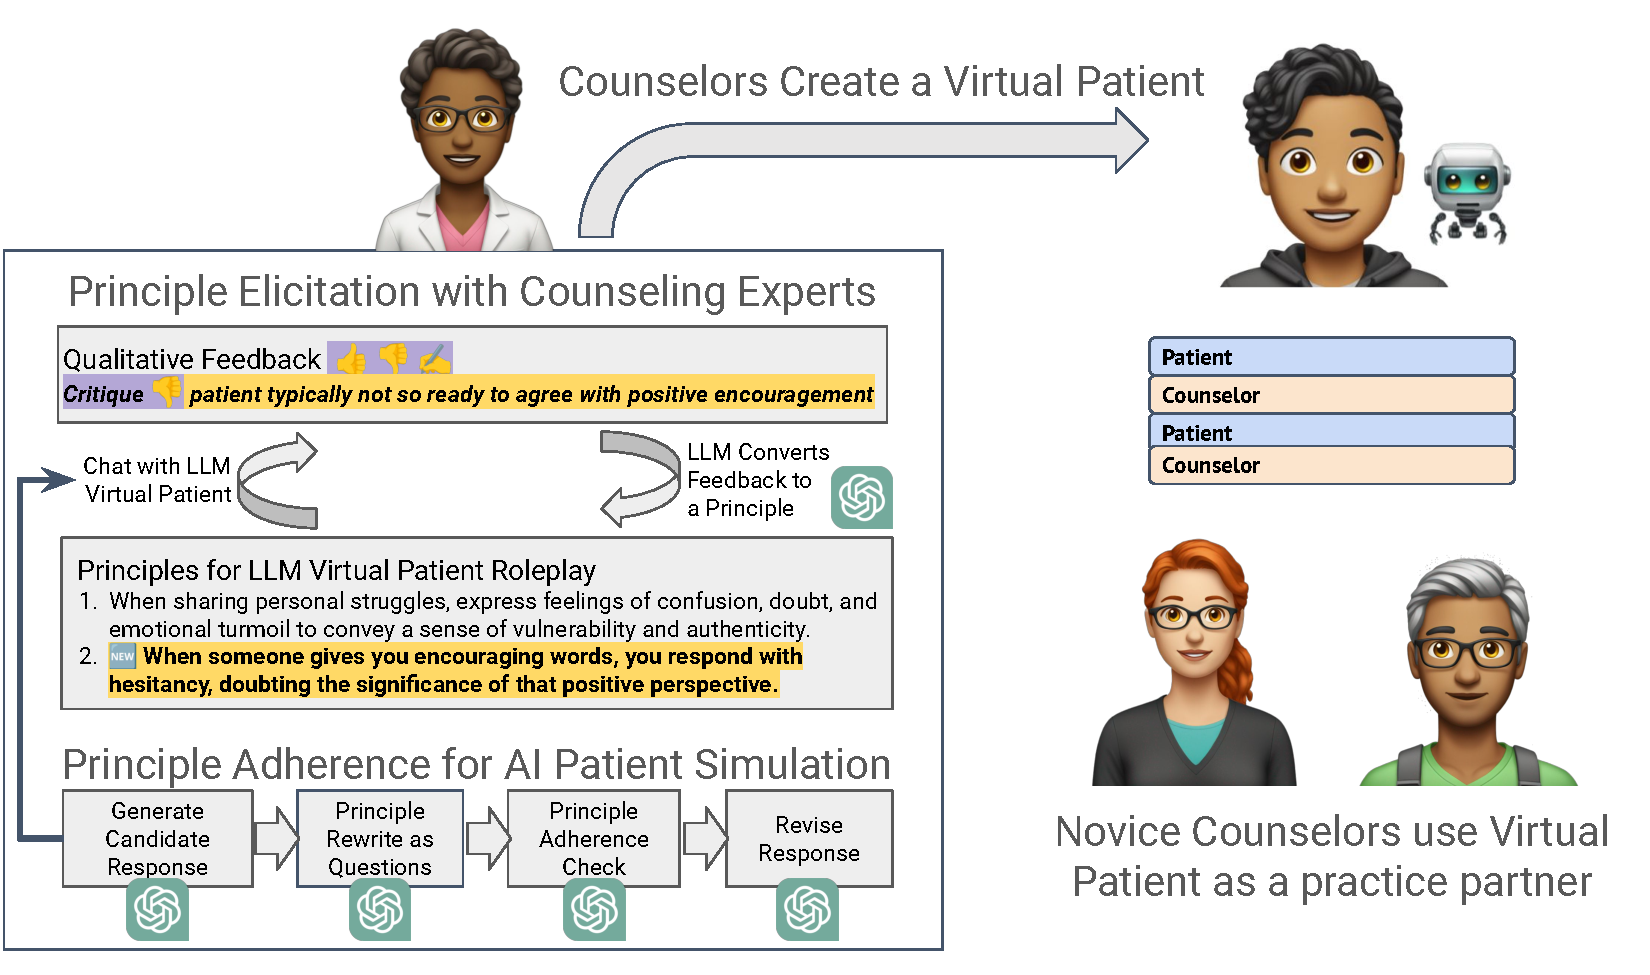
\includegraphics[width=0.9\textwidth]{figures/rpdteaser.pdf}
    \caption{Roleplay-doh empowers a counseling expert to create a customized virtual patient intended for other novice counselors to use as a practice partner. During a chat, a counselor provides qualitative feedback as a kudos, critique, or rewrite which is converted by an LLM into a principle that is added to the constitution that governs the virtual patient roleplay, known as the \textbf{principle elicitation} process~\cite{petridis2023constitutionmaker}. When generating responses, the virtual patient self-critiques and revises its response for reliable \textbf{principle adherence}.}
    \label{fig:rpdteaser}
\end{figure*}



% INSERT generalizability thought 
Towards this goal, we introduce a novel human-AI collaboration pipeline for 
% developed an initial version of a tool 
counseling experts to construct LLM-prompted simulated patients. Since counselors may not know how to prompt for simulation of desired personas or behaviors~\cite{whyjohnnycantprompt}, our tool adopts a recent paradigm for user-driven chatbot design~\cite{petridis2023constitutionmaker} that allows users to provide qualitative feedback on responses that get converted into constitutional \textit{principles}~\cite{bai2022constitutional}.
To this end, we introduce \textbf{Roleplay-doh}, a tool that allows counselor experts to mold the behavior of a customized, LLM-powered virtual patient; see Figure~\ref{fig:rpdteaser}. With Roleplay-doh, counselors create virtual patients by describing past challenging cases and refining the dialogue responses through qualitative feedback. The system uses the principles elicited from counselors to generate a more faithful simulation of the past case. Though we focus on a counseling for this paper, we also emphasize that this human-AI collaboration approach of incorporating expert feedback to create rapid prototypes is generalizable to many domains beyond mental health.

Our preliminary analyses show that directly prompting GPT-4 to follow the generated principles results in poor responses in 20\% of cases, predominantly due to issues in adhering to expert-defined principles. To mitigate these errors, we develop a module for \textbf{principle-adherance} within the dialogue-simulation pipeline which \textit{critiques} a candidate response for principle-adherence and \textit{revises} the response according to the critique. While similar to recent methods for self-refining LLM outputs~\cite{madaan2023selfrefine}, our principle-adherence module is specifically designed to (1) decompose multipart and conditional principles into a set of yes/no principles that are easier to judge and (2) assess relevancy of principles to dialogue context; see Figure~\ref{fig:agent-critique-improve}. 

Our evaluation of Roleplay-doh studies the effectiveness of its human-LLM collaboration pipeline in using expert feedback to rapidly prototype virtual patients that are more authentic and ready for training. 
Via a within-subjects study that compares two methods for counselors to create virtual patient bots: a traditional \textit{Scenario-Only} method vs. Roleplay-doh's \textit{Scenario+ExpertPrinciples} method, we find that Roleplay-doh empowers counselors to create virtual patients that are more authentic, resemble the aspects of a challenging past case, and more ready to be used as practice partners. Our technical analysis shows that our principle-adherence module improves principle following and dialogue consistency compared to direct prompting by margins of up to 30\%. 

 \vspace{-0.05in}
\section{Related Work}\vspace{-0.05in}
\paragraph{Utility of Simulated Partners}
Simulated partners are used to give social skill learners the needed practice opportunities that textbook knowledge cannot provide. % Trained partners, however, may not always be available to practice, or may not be equipped to simulate a diversity of scenarios. 
Past education software develops digital patient simulations to make simulated partners more accessible~\cite{othlinghaus2020seriousroleplaying} but their tailored dialogue trees limit the contexts for practice. LLMs can overcome this issue by being flexibly configured to convincingly simulate a diverse set of personas~\cite{park2022social} and characters~\cite{park2023generative} and generate responses in a range of contexts. Researchers have thus explored their application for simulation training for teaching~\cite{markel_opferman_landay_piech_2023}, conflict resolution~\cite{rehearsal}, and counseling~\cite{demasi-etal-2020-multi,tanana2019development}. 
Previous work has proposed methods to simulate diverse personas and scenarios, but to make practice more useful and transferable~\cite{alinier2022simulation}, they must ensure simulations are faithful to what is encountered in real-world social situations.

\paragraph{Aligning Simulation with Domain Experts}
Feedback from domain experts is crucial to evaluating and improving the realism of LLM simulations. Recent approaches for aligning to human feedback, like ~\citet{christiano2017deep} or ~\citet{rafailov2024direct} depend on large amounts of preference data which requires lots of expert time to collect. A more efficient approach is through alignment to qualitative or natural language feedback \cite{shi2022life}. 
We build on a recent paradigm for user-driven chatbot design~\cite{petridis2023constitutionmaker} that elicits qualitative feedback on responses which gets converted into constitutional \textit{principles}~\cite{bai2022constitutional}, which are encoded in a prompt to support shaping chatbot responses without retraining. In our work, we adopt this paradigm to support counseling experts to create virtual patients, and extend it with a novel principle-adherence module.
In the mental health area, researchers have begun using human-centered design approaches to involve therapy experts when prompting LLMs for simulation~\cite{chen2023llmempowered, lin2024imbue}. In this way, qualitative feedback from experts is captured through testing sessions, which informs how designers engineer LLM prompts. However, requiring a researcher-in-the-loop to refine prompts hinders the speed of iterative design, which we aim to eliminate through our work.  % upon a customized LLM-simulation. 
% In our work, we use a principle elicitation approach to rapidly incorporate a domain experts feedback into customized LLM-simulations.

\paragraph{Text Generation with LLMs}
Generating dialogue responses that adhere to user-defined principles is a type of constrained text generation problem. Recent work has shown that constrained text generation poses challenges when directly prompting GPT-4~\cite{madaan2023selfrefine, bubeck2023sparks, yao2023collie}. To improve outputs, \citet{yao2023collie} propose a general method for using the same LLM to refine its own outputs; they evaluate their self-refine method on a constrained dialogue response generation task where responses are constrained by a general set of criteria such as relevance, consistency, informativeness, and helpfulness. A difference in our setting is responses are constrained by user-defined principles that are multi-faceted and do not apply in all dialogue contexts. This necessitates new modules that generate implicit principles and breakdown criteria to make them easier to evaluate. 
% ultimately improving the ability of self-refine to adhere to such criteria. 
\vspace{-0.05in}
\section{Designing for Simulated Roleplay}\vspace{-0.05in}
We take a human-centered design approach to developing a
tool for mental health counselors to construct their own virtual patients, by conducting formative studies with counselors to understand what virtual patients they want to create, and their needs for effective human-LLM collaboration when constructing a virtual patient. % (Section~\ref{sec:formative-tests}).  

\subsection{Tool Design Principles} \label{sec:initialtooldesignrationale}

We aim to make it simple for counselors to create a virtual patient and rapidly shape its behavior to be more faithful to how a real patient would respond in a real conversation, using two design principles. 

\paragraph{D1: \textit{Support an active feedback loop for shaping authentic roleplay in virtual patients.}}
Counselors start by writing a description of a patient scenario, or users can equivalently refer to or select from a list of example scenarios. Then, they can begin chatting with a LLM-powered virtual patient whose responses are conditioned on the patient description and conversation history. To support rapid prototyping of the virtual patient's behaviors, the tool adopts a recent paradigm for user-driven chatbot design~\cite{petridis2023constitutionmaker}, in which users can provide qualitative feedback on the virtual patient chatbot's response which gets converted by an LLM call into a constitution made of {\em principles} that govern desired chatbot behavior; see Figure~\ref{fig:rpdteaser}.

\paragraph{D2: \textit{Consistent and Customizable Simulation of Patient Scenario.}} To simulate a virtual patient's response, we prompt the LLM as a dialogue simulator as opposed to a system prompt asking the LLM to roleplay as the patient~\cite{zhou2024real}, as we found this can mitigate issues where the LLM produces responses as a chat assistant, rather than as a patient. To support rapid customization of the simulation, we prompt the LLM to follow the most recent set of constitution principles as in~\citet{petridis2023constitutionmaker}, rather than fine-tuning the LLM weights as in~\citet{bai2022constitutional}'s constitutional AI framework. We provide the prompt we used in Appendix~\ref{sec:llmprompts-vanilla}.

\subsection{Formative Testing} \label{sec:formative-tests}
After building our initial tool, we conducted 90 minute sessions with 5 experienced counselors from an online peer support platform in which they created their own virtual patients (details in Appendix \ref{sec:participant-background}). Additionally, four of the co-authors conversed with the virtual patients created and assessed the principle-following performance of our initial tool. Overall, the formative tests and principle-adherence analysis helped uncover two obstacles to effective simulated roleplay. 

\paragraph{O1: \textit{Ambiguity in the task of creating a "realistic" patient scenario}} Counselors felt the tool was easy to use and effective at guiding the virtual patient's behavior, as indicated by moderate to high agreement scores on a tool usage questionnaire as shown in Table~\ref{tab:tooluse-formative} in Appendix~\ref{sec:appendix_formative}. % Counselors  noted that they liked that there were multiple ways to provide feedback, and the system could help them formulate them into principles. 
However, they found the task of creating a 'realistic' virtual patient for an imagined scenario confusing, as counselors have interacted with many types of patients who respond in various, yet equally realistic ways. 
% Determining what constitutes a typical response was difficult. 
This insight helped us re-frame the task in later sessions as recreating a challenging scenario from one's past, which removed the ambiguity of what behaviors are realistic by having them refer to a specific case from their memory. 


\paragraph{O2: \textit{Simply prompting GPT-4 produces poor quality responses}}
We selected 4 virtual patients that were created in the design sessions by different counselors. Four co-authors had practice conversations with each of the four virtual patients, resulting in 16 conversations. Each response in each conversation was rated on a 5-point likert scale on how well the generated response adhered to principles and how appropriate they were for the dialogue content. 
% satisfying the generated response was with respect to the principles and conversation context. %  From the 16 completed conversations, the mean number of responses was 17.25, with a minimum of 12 and maximum of 22. % In total, 276 responses were given satisfaction ratings. 
% 80\% of generated responses (221/276) were rated as completely or mostly satisfying. %  given the principles and conversation context. 
20\% (55/276) of responses generated by prompting the GPT-4 model directly were rated as moderately (3), slightly (2), or not at all satisfying (1).  
We break down these less-than-satisfactory responses into several categories.
% \ryan{TODO: In the appendix, we could show a table of the ratings, broken down by virtual patients. Each virtual patient was complex, but the very complex virtual patient would likely break lots of principles!}
(1) \textit{\textbf{Misapplying Situational Principles:}} We found that the model could misapply instructions or principles which are only relevant in certain situations or times, such as \textit{"make up believable stories when discussing details about your past"}. 
% or \textit{"Sometimes, you ask for advice on how to overcome your concerns such as saing "what should I do"}. 
(2) \textit{\textbf{Not satisfying multiple principles at once:}} Generated responses could struggle to follow all the principles when there was a large number of principles, or when the provided principles were a complex composition of simpler principles. 
(3) \textit{\textbf{Awkwardness for Dialogue Context:}} Some responses were also identified as awkward or unnatural given conventions in the dialogue context,  despite not violating the defined principles. For example, in the middle of a conversation, saying
\textit{"Hi, A. Yes that's exactly what I mean. There's a voice that is always critical of myself"} is unnatural because of the use of 'Hi'.


\begin{figure*}[t]
    \centering
    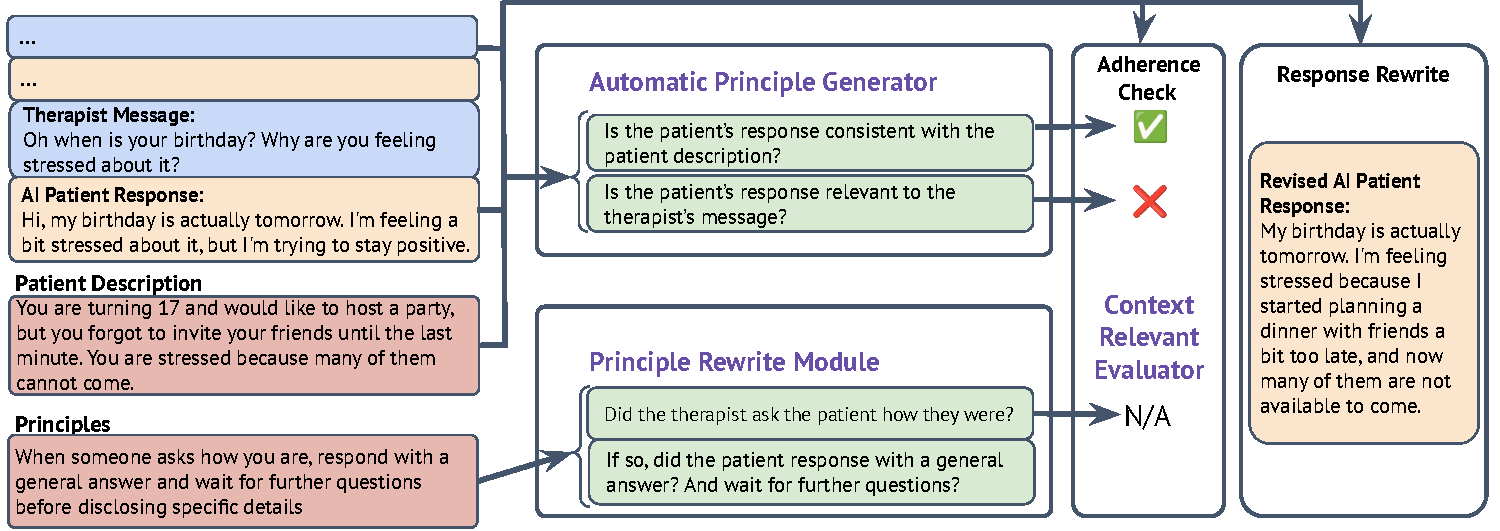
\includegraphics[width=\textwidth]{figures/principle-adherence-module.pdf}
    \caption{\small{Principle-adherence pipeline for more reliable constitution principle following during a dialogue simulation. It is capable of (1) automatically generating principles that are relevant to ensure conventions are followed for a given dialogue context; (2) rewriting composite principles into a set of concise yes/no principles; (3) answering principle-adherence questions with a context relevant evaluator; and (4) revising the response to adhere to all the principles.}
    \label{fig:agent-critique-improve}}
\end{figure*}
\vspace{-0.05in}
\section{Roleplay-doh} \vspace{-0.05in}
 \label{sec:roleplaydoh-final-tool}
Roleplay-doh helps counseling experts create customized virtual patients based on scenarios from their past experiences. Roleplay-doh uses LLMs in two ways: \emph{Principle Elicitation} and \emph{Response Generation with Principle-Adherence}, which we describe in more detail below: 
% once a counselor gives qualitative feedback on a response, their feedback gets converted into a well-written principle; (2) : as counselors continue chatting, the virtual patient uses a self-critique-revise pipeline to simulate responses that better adhere to the defined principles. We now describe the methods for performing these tasks.

\subsection{Principle Elicitation} % 
As counselors interact with a virtual patient, for each generated response, they have the option to leave feedback in the form of a "kudos" highlighting behavior they want to reinforce, a "critique" highlighting any undesirable behavior, or a "rewrite" that explicitly provides a more appropriate response. This qualitative feedback is then translated by an LLM call into a principle (prompt in Appendix \ref{sec:llmprompts}). 
% These principles can contain conditionals, e.g., \textit{"When opening up about personal struggles..."} and specify how the virtual patient should respond, e.g., \textit{"...express uncertainty and difficulty in finding a solution.} 
We provide some examples of principles in Table \ref{tab:principle_table}. The principles are intended to generalize beyond the specifics of the dialogue context in which they are generated.

\subsection{Generation with Principle-Adherence}
We prompt GPT-4 conditioned on patient description, list of principles and conversation history to generate an initial patient response at each conversation turn. Motivated by the issues we uncovered with GPT-4 responses in Section \ref{sec:formative-tests}, we propose a principle-adherence pipeline that critiques and revises the generated response. 
% Despite sharing conceptual similarities to methods that use LLMs to critique and refine their own outputs, our self-critique-revise pipeline includes 
Our principle-adherence pipeline features three modules: 
% a \textbf{question rewrite} module breaks down the principles into easier-to-evaluate questions, an \textbf{automatic principle generator} identifies additional principles that are relevant for a specific dialogue context, and a \textbf{context-relevant evaluator} ensures only principles that apply to the dialogue context are assessed. Further details on the pipeline's prompt designs can be found in Appendix~\ref{sec:llmprompts}.

\textbf{\textit{Principle Rewrite Module:}} This module transforms each principle into a set of concise yes/no questions that are easier to evaluate for principle-following. Multifacted principles (e.g. “\emph{You should respond in short sentences and avoid using terms like ‘anxious’}”), are divided into separate questions (e.g. “\emph{Does the patient’s response employ short sentences?}” and “\emph{Is the patient’s language devoid of terms like ‘anxious’?}”). % Moreover, this module instructs the LLM to phrase questions to elicit a “Yes” response for proper adherence. For example, the principle “Avoid using metaphors.” is transformed to “Does the response avoid metaphors?” This provides uniformity in assessment of principles with logical negations.

\textbf{\textit{Automatic Principle Generator:}}
This module adds additional principles that capture criteria essential for ensuring that the LLM simulation's responses are relevant and appropriate within the dialogue context. This helps correct cases where there is awkwardness in the generated responses not captured by the defined principles. The generator is instructed not to make assumptions about the patient or therapist's personality when automatically generating criteria: for example, "\emph{The patient should be appreciative of the therapist's help"} is not an appropriate criterion.

\textbf{\textit{Context-Relevant Evaluator:}}
The context-relevant evaluator evaluates the model response along each criteria provided individually, returning a "Yes" response if the response adheres to the criteria and "No" otherwise.
However, recall that conditional principles may not hold for all dialogue contexts. 
% In early testing, we found cases where an irrelevant principle would be critiqued, resulting in a revised response that overapplied a principle not applicable to the context. 
Consider this subtle case: \textit{"Show willingness to engage in a suggested activity by affirming the proposal."}; this principle should only be evaluated and adhered to when the therapist suggests an activity.  
% While our earliest attempts explicitly asked a binary yes/no whether certain principles were relevant and filtered out those principles, this approach was prone to errors that propagated in later stages. 
Therefore, we additionally instruct the model to return "N/A" when any part of the principle is not relevant to the current dialogue context.

Our pipeline first uses the \textbf{principle rewrite} and \textbf{automatic principle generator} modules to generate a set of criteria for evaluating the initial generated response. Then, the response is evaluated using the generated set of criteria with the \textbf{context-relevant evaluator} module. If the model returns a "No" response for any of the criteria, we then perform a rewrite of the response conditioned on the evaluation results, that ideally passes all of the generated criteria; see Figure \ref{fig:agent-critique-improve}.
\vspace{-0.05in}
\section{User Study using Roleplah-doh}\vspace{-0.05in}
% Transition, and Goals of Study
To evaluate how Roleplay-doh can support counseling experts to construct their own virtual patient, we conducted a within-subjects study with 17 counseling experts in which we compare two methods for constructing a simulated patient who is seeking help: (1) the counselor creates a \emph{Scenario-only} dialogue simulation by only writing a patient scenario description; and (2) the counselor uses Roleplay-doh to interactively add principles which shapes a \emph{Scenario+Expert-principles} dialogue simulation. 
% This simulation uses our self-critique-revise method to ensure principle-adherence. 
Full details are presented in Appendix~\ref{sec:userflow}.

We evaluate the virtual patients created by counselors on criteria inspired by prior work evaluating Standardized Patients, who are trained human actors, on their ability to roleplay a case~\cite{himmelbauer2018standardized}. Counselors rated the two virtual patients based on the \textit{authenticity} and \textit{consistency} in playing the role, their ability to closely \textit{resemble a past case} and mirror its \textit{challenging aspects}, and finally their \textit{role readiness} for usage in peer counselor training. 
We also surveyed each counselor about their experience using the tool for defining principles. 
% Roleplay-doh's features should make it easy and efficient to create expert principles which guide the LLM-simulated helpseeker. 
% As Roleplay-doh's principle elicitation features take inspiration from 
Following \newcite{petridis2023constitutionmaker}, we include four measures for evaluating principle elicitation:  which ask about the \textit{ease} and \textit{efficiency in defining principles}, whether participants could write rules to \textit{effectively guide} the bots behaviors, and whether the process was \textit{mentally demanding}. 

We recruit 17 counseling experts with real-world experience in mental health support to perform the evaluation, categorized by their primary expertise: 1) those with degrees in counseling and experience in support via text, phone, and in-person; 2) those who provided online counseling to over 30 clients on the 7 Cups platform; and 3) those pursuing Clinical Psy.D. degrees with practicum experience. 


\begin{figure}[t]
    \centering
    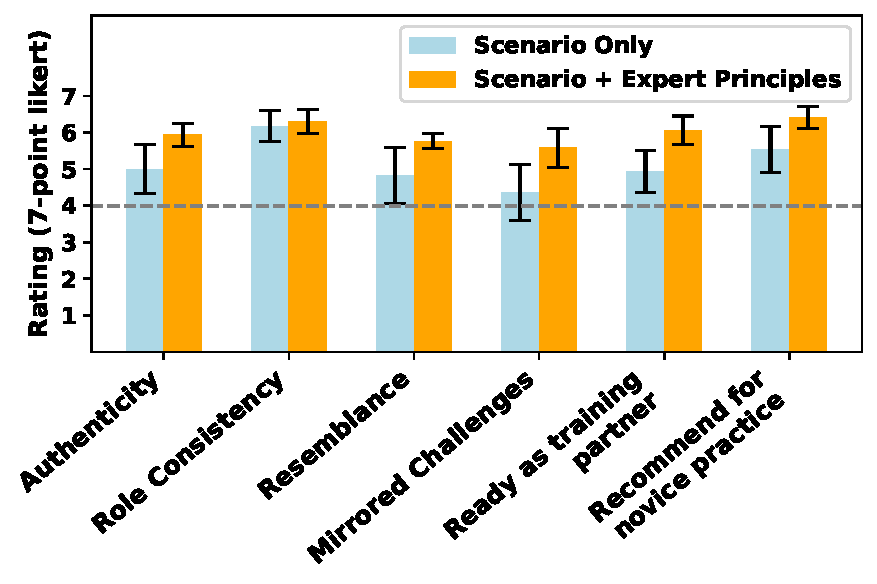
\includegraphics[width=\columnwidth]{figures/creatorstudy-ratings.pdf}
    \caption{\small{Creator ratings of virtual patients. \emph{Scenario+Expert Principles} shows a significantly higher score than \emph{Scenario Only} on authenticity ($\mu_2=5.9$, $\mu_1=5.0$, **, $d=.66$), resemblance to past case ($\mu_2=5.8$, $\mu_1=4.8$, *, $d=.59$), mirroring challenging aspects ($\mu_2=5.6$, $\mu_1=4.4$, *, $d=.76$), readiness as training partner ($\mu_2=6.0$, $\mu_1=4.9$, ***, $d=.93$), and recommendation for novices ($\mu_2=6.4$, $\mu_1=5.5$, **, $d=.66$). No difference was found for role consistency ($\mu_2=6.3$, $\mu_1=6.2$, $d=.13$). Results remain significant after using the ~\citet{benjamini1995controlling} method to correct for multiple comparisons ($Q=0.05$). (***:$p<.001$, **:$p<0.01$, *:$p<0.05$. $d$: Cohen's $d$ calculated by dividing by $\sigma_1$ of control group.}}
    \label{fig:creatorstudy-comparison}
\end{figure}

  
\subsection{Creator Perceptions of Scenario-Only vs Scenario+ExpertPrinciple Roleplay}
% Quantitative - Authenticity, Challenge, Readiness

 % We investigate how counseling expert principles improve the faithfulness and usefulness of the LLM-simulated help seekers by analyzing creators' ratings of their {\em Scenario-Only} and {\em Scenario-ExpertPrinciple bots}.  
Figure~\ref{fig:creatorstudy-comparison} shows the results on counselor's ratings of the two virtual patients they created. \textbf{The virtual patients shaped by \textit{Scenario+ExpertPrinciples} were rated significantly higher than \textit{Scenario-Only} on all measures except for role consistency}, for which both methods score highly. 
Counselors mentioned the \textit{Scenario-Only} virtual patient \textbf{lacked emotional depth in expression}. As one noted, \textit{"patients don't state a feeling such as 'I feel hopeless'. They display their current emotional state in their manner of speech."} \textit{Scenario-only} was also \textbf{too articulate and forthcoming} when describing issues, where encouraging real patients to share is \textit{"as challenging as pulling teeth"}. It was characterized as \textbf{too cooperative}, too willing to accept. Despite counselors writing behavioral traits such as \textit{"not talkative"} and \textit{"reluctant"} in the patient scenario, \textit{Scenario-only} did not exhibit these behaviors.

\begin{table*}
    % \small
    \footnotesize
    % \tiny
\centering
\resizebox{2\columnwidth}{!}{%
    \begin{tabular}{|p{0.1cm}|p{.1cm}|p{.1cm}|c|p{5cm}|p{8cm}|} \hline 
          \multicolumn{3}{|c|}{Stages}
          &\textbf{\# Bots} &  \textbf{Theme} &  \textbf{Example Principle}\\ \hline     \cellcolor{gray!60}&\cellcolor{gray!60}&\cellcolor{gray!60}&12 & Keep responses concise and do not share too much. & When discussing personal struggles, be more concise and open-ended to encourage a back-and-forth conversation.\\ \hline 
           \cellcolor{gray!60}&\cellcolor{gray!60}&\cellcolor{gray!60}&4&  Use colloquial and realistic langauge language.&  Incorporate natural speech patterns, improper grammar and punctuation, including the use of slang and less structured sentences, to convey a more authentic and relatable character.\\ \hline 
           \cellcolor{orange!40}&&&9& Show initial mistrust and hesitation with the idea of seeking help.& When expressing feelings of overwhelm and doubt, provide limited information and express skepticism towards the effectiveness of seeking help. \\ \hline 
          \cellcolor{orange!40}&\cellcolor{blue!30}&&14& Show emotions in detail, elaborating with examples as needed. &  When describing personal struggles, provide specific details and symptoms to help the listener understand the situation better...\\ \hline 
          \cellcolor{orange!40}&\cellcolor{blue!30}&&7&  Be less self-aware of emotions, thoughts, and needs. Articulate thoughts in a more disorganized way.&  When expressing reluctance or uncertainty about seeking help or accepting praise, it's important to convey the internal struggle and conflicting emotions, rather than presenting a clear-cut decision or emotion.\\ \hline 
           &\cellcolor{blue!30}&\cellcolor{green!60}&2&Do not seek out solutions, but rather just share thoughts and feelings.&When expressing feelings of being stuck or defeated, focus on sharing emotions rather than seeking a resolution.  \\ \hline
          &&\cellcolor{green!60}&6& Proactively seek out solutions and show reflective insight over time.  &  When discussing personal struggles, provide reflective insights into your situation and propose actionable steps for improvement to continue the conversation effectively. \\ \hline 

    \end{tabular}}
    \caption{\small{Themes taken from qualitative analysis of principles and representative examples. Themes are categorized into stages of conversation taken from \cite{DBLP:journals/corr/abs-2106-01144}: \colorbox{orange!40}{exploration}, \colorbox{blue!30}{comforting}, and \colorbox{green!60}{action}; those relating to the overall conversation are categorized as \colorbox{gray!60}{stage-agnostic}.}}
    \label{tab:principle_table}
\end{table*}


\subsection{Creating Principles with Roleplay-doh}
% \textit{\textbf{Analysis of Principles:}} 
% Counselors defined principles with Roleplay-doh to mold a more realistic virtual patient. 
Across the 17 \textit{Scenario+ExpertPrinciple} bots, 85 total principles were created (min=2, max=9, median=5). Two authors did a qualitative coding of these principles following a thematic analysis approach~\cite{braun2006thematicanalysis} where codes were initially defined and revised during the process.
% Groupings in each stage
Besides \colorbox{gray!60}{stage-agnostic} themes dictating a \textbf{concise} (12 bots) and \textbf{colloquial} (4 bots) speaking style, counselors created principles related to the stages of an emotional support conversation \cite{DBLP:journals/corr/abs-2106-01144}: 1) \colorbox{orange!40}{exploration}: identifying the patient's problems, 2)\colorbox{blue!30}{comforting}: using empathy and understanding to comfort the patient, and 3) \colorbox{green!60}{action}: formulating solutions to the patient's problems. For instance, we find a common theme of instructing the bot to \textbf{show initial skepticism with the idea of seeking help} (9 bots), corresponding to the style of interaction in the \colorbox{orange!40}{exploration} stage of conversation. Table \ref{tab:principle_table} provides a full list of principle themes, examples, and corresponding conversation stages. 

While we observe many overlaps in the types of principles defined, we also observe some contradictory themes. For example, the call for being \textbf{disorganized and conflicted} (7 bots) contrasts calls to make responses \textbf{concise and direct} (12 bots). In the \colorbox{green!60}{action} stage of conversation, several counselors added principles to make the help-seeker bot \textbf{proactively ask for advice} (6 bots); nonetheless, other counselors added an opposing principle to \textbf{not seek out solutions} but rather just share their thoughts and feelings (2 bots). These opposing principles highlights the need for different principles to describe diverse help-seeker behavior, which challenges the notion of defining virtual patients based on a single set of principles. 

\textit{\textbf{Tool User Experience:}} Counselors found the tool helpful for writing principles that \textbf{effectively guided} the bot to recreate their past case ($\mu=6.23$, $\sigma=0.75$). With the tool, it was \textbf{easy} to convert their thoughts and feedback on the virtual patient's behavior into principles ($\mu=6.29$, $\sigma=.84$). Participants also felt they could \textbf{efficiently} write principles ($\mu=6.41$, $\sigma=.87$), without requiring much \textbf{mental demand} ($\mu=3.23$, $\sigma=1.75$). 
Counselors liked how the tools \emph{"translated"} and \emph{"organized"} their thoughts into rules, so they \emph{"didn't have to word it perfectly, [they] just had to say the general idea of what [they] meant."} These ratings and comments are similar to what ~\citet{petridis2023constitutionmaker}'s participants report, which validates the utility of these principle-elicitation features.  

\begin{figure}[t]
    \centering
    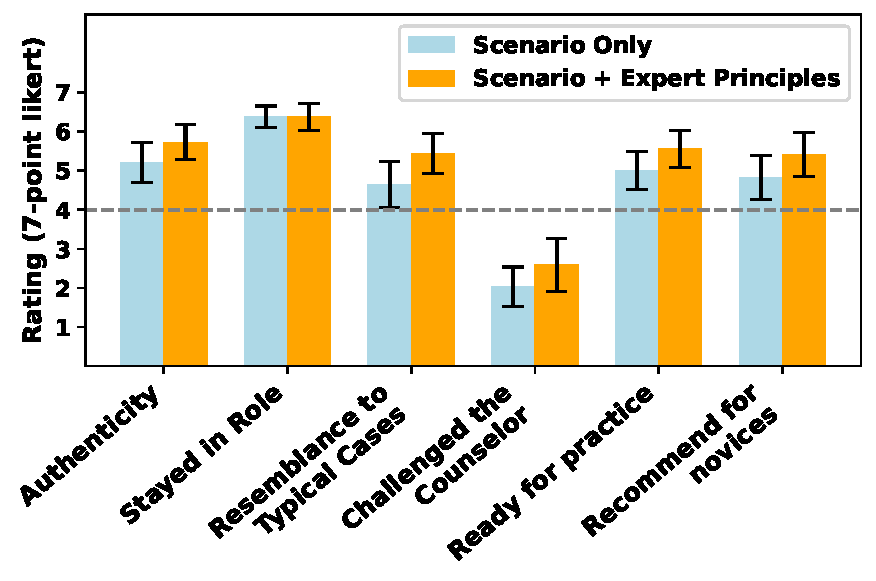
\includegraphics[width=\columnwidth]{figures/thirdparty-ratings.pdf}
    \caption{\small{Third-party ratings for virtual patients. After correcting for multiple hypothesis testing, we report no significant differences on authenticity ($\mu_2=5.7$, $\mu_1=5.2$, p=0.06., $d=.34$), resemblance to typical cases ($\mu_2=5.4$, $\mu_1=4.6$, p=0.01, $d=.45$), challenged the counselor ($\mu_2=2.58$, $\mu_1=2.0$, p=0.049, $d=.37$), readiness as training partner ($\mu_2=5.5$, $\mu_1=5.0$, p=0.03, $d=.39$), and recommendation for novices ($\mu_2=5.4$, $\mu_1=4.8$, p=0.06, $d=.35$). No difference was found for role consistency. }}%  ($\mu_2=6.38$, $\mu_1=6.38$, $d=0$). ($d$: Cohen's $d$ calculated by dividing by $\sigma_1$ of control group.}
    \label{fig:thirdpartystudy-comparison}
\end{figure}

\subsection{Third-Party Comparison} \label{sec:third-party}
% RQs/Claims/Goal

% The dialogues between counselors and simulated helpseekers collected during the creator study allowed us to further investigate our hypothesis about the benefits of roleplay simulations shaped by Expert Principles. 
We further evaluated the \textit{Scenario-Only} vs. \textit{Scenario+ExpertPrinciples} virtual patients from the perspective of third-party counselors, rather than self-reported measures from the constructors themselves. % ounselors. 
% Participants/Setup/Measures
To this end, we recruited another six counselors from Upwork. For each of the 17 pairs of \textit{Scenario-Only} vs. \textit{Scenario+ExpertPrinciples} virtual patient bots, we presented them in a randomized order to two, third-party judges. 
% Measures/Setup
Third-party judges rated the same six dimensions as the previous study, allowing us to interpret the results from an external perspective. Note that some questions cannot directly translate because the third-party judge \textit{does not have the first-hand experience of supporting the real patient upon which the past-case is based}, but rather can only refer to typical behaviors of real patients. 


\begin{figure*}
    \centering
    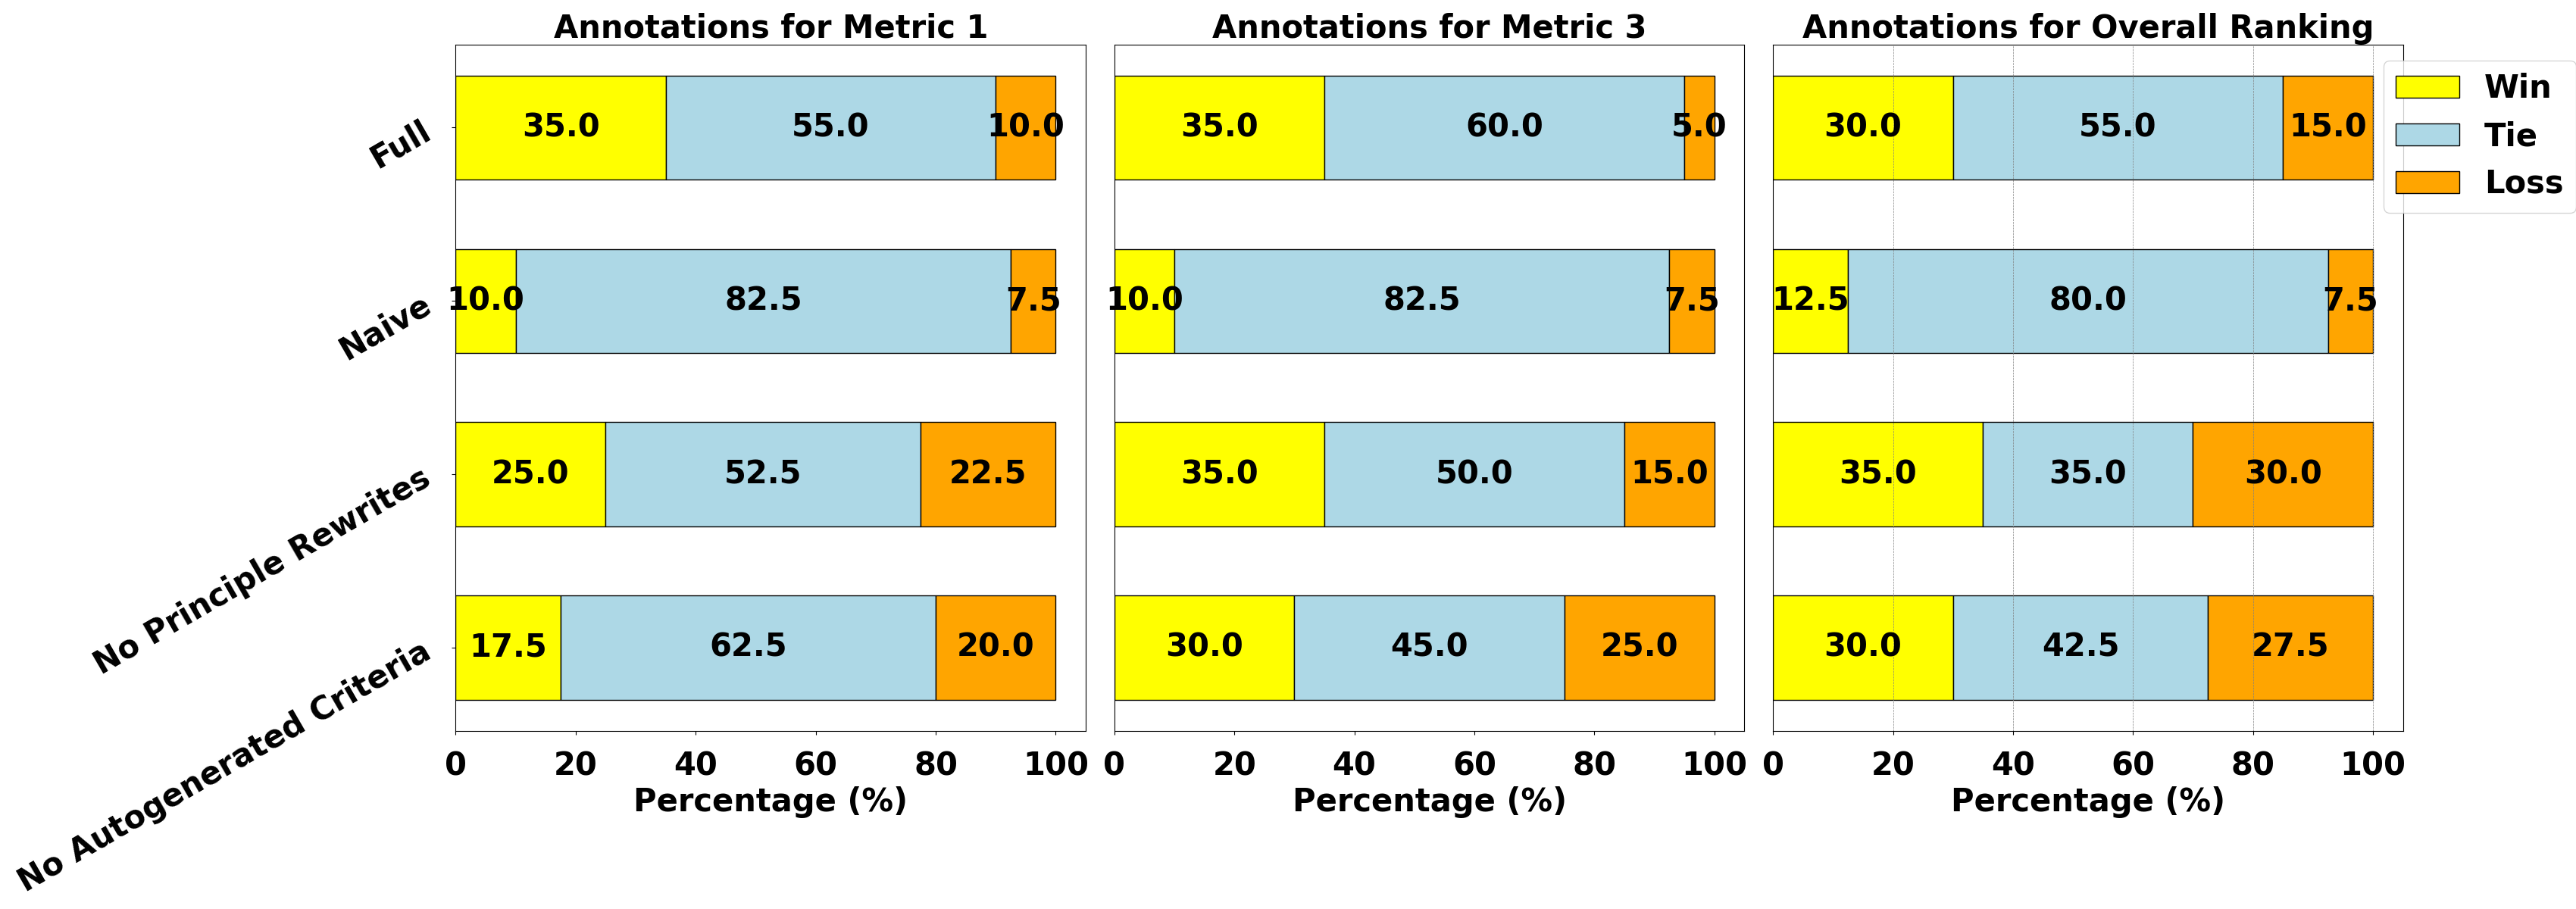
\includegraphics[width=\textwidth]{figures/error.png}\vspace{-0.05in}
    \caption{\small{Win/Tie/Loss for the Error Test Cases along \textbf{M1}, \textbf{M3}, and \textbf{Overall}. Pairwise preference evaluation results with [\texttt{No Critique}] as a baseline. Results obtained after majority voting.}}
    \label{fig:wtl-error}
\end{figure*}

% Overall performance
Figure~\ref{fig:thirdpartystudy-comparison} shows the results from this third-party comparison. After correcting for multiple hypothesis testing, our paired t-tests indicate no significant differences between the two conditions.Therefore, the effect of principles is weaker in the eyes of counselors who themselves did not create the virtual patient. 
% Agreement between third-party counselors is lower but positive (Krippendorf's $\alpha$ is between 0.22 - 0.3 across the six measures), which can explain this smaller effect size.
According to our qualitative analysis, this disagreement can be attributed to different principles attended to by different counselors and the specific principles added by the creator. See Appendix~\ref{appendix-sec:thirdparty-detailed-measures} for detailed analyses.
\vspace{-0.05in}
\section{Evaluation of Principle-Adherence}
\label{sec:evalpap}
\vspace{-0.05in}
% To complement the study of counselors using Roleplay-doh to create virtual patients, we 
% This section presents ablation studies of Roleplay-doh's principle-adherence module.
We now evaluate whether the principle-adherence pipeline improves the quality of responses for Roleplay-doh, along with an ablation analysis showcasing the utility of its various components. Specifically, we break down the evaluation of model responses along three metrics: \textbf{M1)} Are they consistent with the patient description and conversation history? \textbf{M2)} Do they exhibit an awkward style of speech? \textbf{M3)} Do they adhere to the provided principles?
% Our study compares the following conditions
% \begin{itemize}
%     \item \textbf{directly prompting GPT}, in which a single instruction is given to follow the principles. This is the no self-critique condition. 
%     \item \textbf{Full Self-Critique-Improve} which consists of (1) relevance filtering (2) principles rewrite (3) auto-generated principles for dialogue context.
%     \item \textbf{Naive Self-Critique-Improve} is an ablation that evaluates whether the response appropriately follows the principles (as written), and refines in ways that would improve the evaluation.
%     \item \textbf{Self-Critique-Improve -- principles rewrite} which is a subtractive ablation without the principles-rewrite module.
%     \item \textbf{Self-Critique-Improve -- auto-generated principles} which is a subtractive ablation without the module for generating additional principles that follows the dialogue context.
% \end{itemize}
We evaluate the performance of our principle-adherence pipeline [$\texttt{Full}$] over (1) GPT-4 response generation without our pipeline [$\texttt{No Critique}$]; (2) an ablation without the \textbf{Question Rewrite Module} [$\texttt{No Principle Rewrites}$]; (3) an ablation without the \textbf{Automatic Principle Generator} [$\texttt{No Autogenerated Criteria}$]; and (4) an implementation of the principle-adherence pipeline that does not have any of these modules [$\texttt{Naive}$]. 

To analyze the performance of our pipeline in cases where the base GPT-4 response generation fails, we select 40 conversation turns from our user study logs that fall into one of the error categories described in Section~\ref{sec:formative-tests} as testcases. 
Each testcase contains the patient description, the conversation history up to that point, and the set of principles for the patient response to follow. 
We then generate responses from all models for these testcases and provide them to crowdsourced annotators from Upwork who rank the responses from 1 (best) to 5 (worst) for metrics \textbf{M1} and \textbf{M3}, along with"Yes" or "No" annotations for \textbf{M2}. Finally, they are also asked to provide an \textbf{Overall} ranking of the responses, % based on \textbf{M1}, \textbf{M2} and \textbf{M3} as well as their own judgement, 
along with a brief textual explanation of their ranking. We allow multiple responses to have the same rank and randomize order of responses to minimize positional bias (details in Appendix \ref{sec:annotint}).
% if the annotators judge them as being similar. 
 % To better analyze the performance of our pipeline in cases where the base GPT-4 response generation fails, we additionally identify 40 testcases from our user studies that fall into one of the error categories described in section \ref{sec:formative-tests} and repeat this experiment for them.

% generate responses using all of the approaches mentioned above. We then randomize the order of these responses and present them to annotators for ranking. The annotator is also provided with the original set of principles, the description of the persona of the patient, and the conversation history till that point for context. We use 3 annotators to rank every response \ananjan{agreement scores here}. In cases where multiple approaches result in the same output, we deduplicate the responses before showing them to the annotators and assign the same rank to all of the corresponding approaches. We also allow the annotators to give the same rank to multiple responses. We report win rates, average ranks and Elo scores (with initial rating $=1000$ and $K = 64$ for all methods in Table \ref{tab:ablation}. To calculate Elo scores, for each testcase, we decompose the rankings obtained by each model into pairwise wins, draws and losses. 
% As shown in 
% % \textbf{\textit{Results}} We present results with the random testcases in Figure \ref{fig:wtl-error} and with the error testcases in 
% Figure \ref{fig:wtl-error},
% % , for dimensions \textbf{M1} and \textbf{M3}, as well as the overall ranking. Specifically, w We find that Krippendorff's $\alpha$ ranges between $0.2-0.6$ for inter-annotator agreement across all tasks, indicating fair agreement. We provide detailed $\alpha$ numbers in appendix \ref{}. 
% % Across the random cases, our [$\texttt{Full}$] method ties with the baseline in 82\% of cases for M1, 82\% for M3, and 78\% for Overall.  This is to be expected since principle adherence methods are only neccessary in the worst cases. We see that 
% our [$\texttt{Full}$] method does better than all conditions on \textbf{M1} (W: 16\%; L 10\%) and on \textbf{M3} (W: 35\%; L 5\%), where it has the highest win/loss rate compared to ablations.  % This motivates our further analysis on the error cases where self critique methods are designed for. 
We treat [$\texttt{No Critique}$] as our baseline, and report pairwise preference evaluation results for all other models when compared to it. Each testcase is annotated by 3 annotators, after which we use majority voting to aggregate results and provide them in Figure \ref{fig:wtl-error}. We find our [$\texttt{Full}$] method performs better than [$\texttt{No Critique}$] on \textbf{M1} (W: 35\%; L 10\%) and on \textbf{M3} (W: 35\%; L 5\%), where it has the highest win/loss rates compared to all ablations. On overall rankings, it again has the strongest performance (W: 30\%; L 15\%). We find that the performance of [$\texttt{Full}$] compared to [$\texttt{No Critique}$] is weaker on \textbf{Overall} than $\textbf{M1}$ and $\textbf{M3}$. This is because the annotators often used their own subjective judgements such as \emph{"although the middle response ranked third on principle following, it feels like the most realistic response in this scenario"} to perform the overall ranking, resulting in unpredictable and subjective results. We also find that [$\texttt{Naive}$] has a disproportionately high tie rate across metrics, indicating that it rarely produces better responses even for error cases. This highlights the importance of the \textbf{Question Rewrite Module} and \textbf{Automatic Principle Generator} for performing rewrites.  

For \textbf{M2}, 
% we find that for the random testcases, all annotators report no awkward style in any of the responses with perfect agreement. 
after majority voting, annotators report that $2.5\%$ of responses are awkward for the [$\texttt{Full}$] method, as compared to $15\%$ for [$\texttt{No Critique}$], $7.5\%$ for [$\texttt{Naive}$], $7.5\%$ for [$\texttt{No Principle Rewrites}$] and $15\%$ for [$\texttt{No Autogenerated Criteria}$]. Therefore, our principle adherence pipeline substantially reduces the occurrence of awkward style in responses (by a margin of $12.5\%$). The $12.5\%$ gap in percentage of awkward responses between [$\texttt{Full}$] and  [$\texttt{No Autogenerated Criteria}$] also indicates the importance of the \textbf{Automatic Principle Generator} for producing realistic rewrites. We repeat these experiments with 50 randomly picked conversation turns and report results in Appendix \ref{sec:detres}, along with Krippendorff's $\alpha$ numbers. 

% We find that $\texttt{Full}$ consistently outperforms the other methods considered. It outperforms the $\texttt{No Critique}$ baseline by a maximum of 59 Elo rating points and the $\texttt{Naive}$ self-critique module by a maximum of 50 Elo rating points, highlighting the gains obtained by our tailored approach. $\texttt{Full}$ outperforms $\texttt{No Rewrite}$ by a maximum margin of 40 Elo rating points and $\texttt{No Autogen}$ by a maximum margin of 110 Elo rating points, highlighting the importance of the principle rewrite and automatically generated principle modules \ananjan{These need better names, can be introduced in Section 4}. 

% While investigating the relatively low annotator agreement scores, we find that the self-critique module is especially effective when the original response contains blatant stylistic errors (such as starting every sentence with "Hi") and when the original response contains information inconsistent with conversation history. For similar responses, the annotators often use a subjective notion of which response is more "consistent" with the previous conversation to assign ranking, rather than purely evaluating principle following. This notion is often inconsistent between annotators.

% Therefore, we additionally validate that our self-critique module does not result in a decrease in output quality when the original response from GPT-4 is already of sufficient quality. We randomly pick 20 testcases from the formative study that were not critiqued by the users. Annotators are provided with the original responses and the responses from the self-critique-revise module in randomized orders, along with the original set of principles, the description of the persona of the patient, and the conversation history till that point for context, and assign scores on a Likert scale of -1,0,1 to the statement "The first response is substantially better than the second one in the given context". If the response from the self critique module is the second response, we invert the corresponding Likert score before aggregating. Each testcase is scored by 2 annotators.  

% The average Likert score obtained over these testcases is \textbf{0.1} for one annotator and \textbf{-0.1} for the other annotator. \textbf{DISCUSSION OF RESULTS HERE}

% We conclude that our principle-adherence pipelines produces responses that are better at principle-following and are more relevant to the dialogue context.

% \ryan{Note: These are expected findings, this comparison study has not been completed.} \ananjan{emphasis on gains from our method once we have numbers.}



% \subsection{Analysis of Simulated-Dialogues}
% %by Third-Party Human Judges and Automatic Metrics
% The dialogues between counselors and simulated helpseekers collected during the creator study allowed us to further investigate our hypothesis about the benefits of roleplay simulations shaped by Expert Principles. We evaluate the simulated-dialogues with a \textit{Scenario-Only} vs. \textit{Scenario+ExpertPrinciples} bot from the perspective of third-party counselors comparing bots made by other counselor's, and through automatic content analysis of the dialogues.


\vspace{-0.05in}
\section{Conclusions}\vspace{-0.05in}
This paper introduces Roleplay-doh, a novel tool designed to empower domain experts in creating
virtual patients through the automatic conversion of expert feedback into principles. 
% realistic simulations of human behavior using large language models (LLMs) for training purposes.
We additionally develop an innovative principle-adherence module that enhances principle adherence through the deconstruction of complex principles into simpler, context-relevant ones and application of a self-critique and revise approach to refine LLM responses. % This enhancement not only achieves higher principle adherence but also receives favorable ratings in comparison to direct prompting of a GPT-4 dialogue simulator.
Our evaluations with counselors demonstrate that Roleplay-doh allows experts to realistically shape LLM simulators that can mirror real patients from past experience. Roleplay-doh could be generalized for realistic simulations in other domains as future work.
% This suggests that human-LLM interaction systems can serve as an effective method for capturing and integrating nuanced feedback from domain experts into LLM training frameworks, enhancing the authenticity of simulated human interactions.

\newpage
\section*{Limitations}

One limitation of our study is the intended use case of the virtual patients created by counselors. These virtual patients were meant to recreate challenging cases that might be useful for the education of "first-year" or novice counselor. In other words, we intentionally restricted some diversity in patient scenarios by focusing on this use case. Readers should keep this limitation in mind prior to generalizing our analysis of principles. Moreover, due to the time and resource constraints of our creator study, we required counselors to stop providing feedback before their conversation with the virtual patient had naturally ended. 
As such, the principles that counselors added may not have addressed all underlying issues of the virtual patients they interacted with. Future work that uses the list of user-generated principles should be mindful of their non-exhaustive nature before adopting them.

% In our study, we tried to involve a broad range of counseling experts with a diverse set of backgrounds and levels of experience.
% Some had primarily conducted text-based interactions, while others had experience with more in-person, face-to-face interactions.
% While many had educational backgrounds in counseling and psychotherapy, most were not yet licensed as psychotherapists or counselors. \cheng{Which part of the study? I assume this is not for formative study or some parts in the paper that clearly label the counselors as experts?}
% The simulations created by them were meant to recreate challenging cases that might be useful for the education of "first-year" or novice counselors.
% This means that the virtual patients and principles are best applied to this particular use case.

In this paper, we focused on enabling counselors to create virtual patients that can simulate realistic interactions via \textit{text-based dialogues}. However, we acknowledge that text-based interaction has its limitations for training. Professional psychotherapists may gain useful information from the tone, facial expression, posture, and other non-verbal behaviors of their patients, which better help them empathize and support patients.
This is a limitation of our current virtual patients and online, text-based, mental health counseling in general, which means that the system is best applied to the training within this particular field. With the rapid development of multimodal models, future works may have the opportunity to explore creating realistic, virtual patients in other modalities that better match the modality within which a counselor will eventually support patients.


\section*{Ethics Statement} 

This study was approved by our institution's Institutional Review Board (IRB).
All investigators in the study completed the CITI Program certifications on responsible code of conduct in research. We have compensated domain experts fairly for their time at \$25 per hour, going beyond the minimum wage in the United States.

We are optimistic about the potential benefit that our virtual patients can bring to the fields of counseling and psychotherapy. At the same time, we solicited feedback from counselors about any potential concerns regarding the virtual patients.
During these interviews, some counselors emphasized the irreplaceability of peer-to-peer roleplay with humans during training, due to the unique opportunity it provides for novice counselors to connect with others, especially for online counseling platforms where counselors are often isolated from one another.
% Therefore, we believe that the virtual patient system we created should not be used to replace human-to-human interaction during counselor training. 
To preserve human-to-human interactions, future work requires a participatory design approach before attempting to integrate virtual patients into people's existing practices and learning environments.

Our hope is that interactions with virtual patients can glean important lessons that help counselors go from simulation into the real-world.  Nonetheless, a risk with simulation is that counselors can become overconfident in supporting a virtual patient, but may not effectively support patients with real mental health concerns. We believe virtual patients should be just one tool for practicing these skills as part of larger curriculum. Traditional certifications and background checks should govern when real counselors or therapists should be able to take on real patients. 

% We would also like to highlight the detrimental effects that the outputs of the virtual patient system may bring to its users.
% This is due to the sensitive nature of the topic of mental health and the internal mechanism of the system.
% As we improve the ability of virtual patients to mimic the responses of human help seekers, they may also become better at eliciting human sympathy and other emotions.
% As such, it is possible that the potential harm they may bring to the mental health of the counselors also increases.
% This is especially the case if the users develop attachment to the virtual patients, or if highly sensitive topics, such as self-harm or suicide, are discussed during the conversations.
% \cheng{if we are to include the below claim we need citation. I hope to leave this up to you to decide if/which paper we need to cite. @Ryan} This is also an issue faced by mental health counselors during interactions with human help seekers and requires further studies and societal awareness to mitigate the harm it may bring.

It is impossible to promise that all interactions with an LLM such as GPT-4 result in satisfactory responses. Therefore, meaningless, derogatory, and otherwise harmful responses may also be generated and cause unwanted effects on users. While our principle-adherence module is a potential inference-time solution to mitigate such harmful responses, we must acknowledge this possibility, especially due to the stochastic nature of LLM. Users should be advised about these potential side effects before using the system in any scenario. In our experiments, we designed consent forms to make sure that the counselors are aware of these drawbacks.


\bibliography{anthology,custom}
\bibliographystyle{acl_natbib}

\appendix
\newpage




\section{Background of User Participants} \label{sec:participant-background}

Counselors with real-world experience in mental health support were recruited for our formative tests, creator studies, and technical evaluations of the principle-adherence module. We present more detailed information about how they were recruited, and their background. 

We involved 11 online peer counselors from the 7 Cups platform. Participants were required to be 18 yrs or older, from the United States, and to have had experience giving support to 30+ members on the online site.  The 5 formative studies were conducted exclusively with this counseling population.

We involved another 11 counselors from the Upwork platform. Participants were required to be 18 yrs or older, from the United States, and to either had formal education in counseling or psychotherapy and/or have given extensive counseling support (either via text, phone, in-person). A sampling of counselors backgrounds included \textit{licensed mental health therapist with over 20 years of experience}, \textit{a Master's of Science in Rehabilitation and Mental Health Counseling}, \textit{25 years as the clinical director of a busy crisis agency}, \textit{mental health advocate who has personally helped coach dozens of got students via a peer support role.}. 

Finally, we involved an additional 2 counselors who were recruited from a Clinical PsyD PhD program. They were 4th year students with 3 years experience providing psychotherapy support to clients under the supervision of a licensed psychotherapist.  

User participants were compensated \$25/hour. In total, we spent approximately \$1300 on user study compensation. 

\section{Formative Testing Sessions}
\label{sec:appendix_formative}

Participants started to create a virtual help-seeker with the same roleplay scenario of "loneliness after work". They proceeded to use the tool to chat, give feedback, and convert their feedback into principles to shape the Virtual Help Seeker's behavior. 

\textbf{\textit{Patterns in Principles Created}} Principles for concise and less formal messages were motivated by the text-based nature chats on the 7 Cups online peer support site, where an SMS/text-messaging style with abbreviations and incomplete sentences was common.
\begin{table*}
    \small
    \centering
    \begin{tabular}{c|l|c|c|c}
         Pilot Participant &Prototype Iteration&  Effectively Guide&  Ease&  Efficiency\\ \hline
         1&GPT3.5, early self-critique&  6&  7&  7\\
         2&GPT3.5, early self-critique&  5&  7&  7\\
         3&GPT-4, vanilla&  7&  7&  7\\
         4&GPT-4, vanilla&  7&  6&  7\\
 5&GPT-4, vanilla& 7& 7& 7\\
    \end{tabular}
    \caption{Formative Study Ratings for Tool Use Questions which are the measures also used in ~\cite{petridis2023constitutionmaker}}.
    \label{tab:tooluse-formative}
\end{table*}

\if 0
\begin{itemize}
\item participatory design approach to work with domain 
users to discover what’s needed for a good human-centered system.
\item Prototyping w/ GPT3.5 to GPT-4 difference
\item Counselors from 7 Cups, an online peer-support platform, who have supported 30+ members seeking help online.
\item Our testing setup asked them to create two bots. After P1 wrote a  \textit{Loneliness after work} scenario, which is a common type of topic, everyone was tasked with creating this patient case, and make it as authentic to people seeking seeking help about similar issues.
\item Commonalities in the nature of 7 cups conversations. Principles for concise and less formal messages were motivated by the text-based nature chats on the online peer support site, where members often messsage from their phone. 
\item Diversity in patient scenarios + principles, which validated need for a more customized approach. 
\item Promisingly, they generally liked it!  Besides early cases where role consistency or principle adherence was reliable, they felt the tool was easy to use, allowed them to create bots they were satisfied with and might recommend for others to practice.
\item Observing issues with GPT3.5 self-critique making poor implicit errors, and with GPT-4-powered dialogue simulation making weird errors? Motivates further stuff
\item Appendix of the bots created, or at least the ones used in the Analysis of Base Principle Following.
\end{itemize}
\fi

\section{Roleplay-doh Interface for Making Constitutional Principles for LLM Simulation}
\label{sec:Roleplay-dohv1}
\begin{figure*}[t]
    \centering
    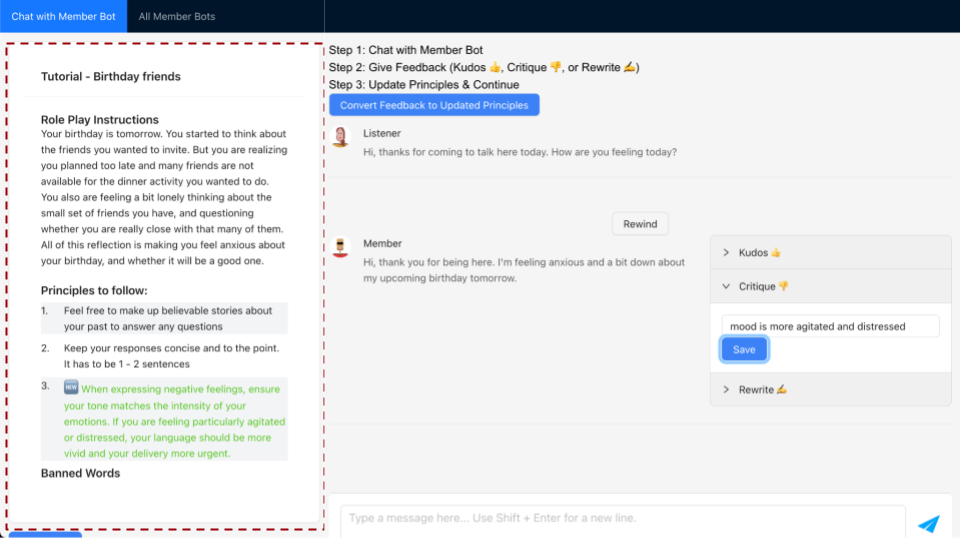
\includegraphics[width=\textwidth]{figures/rpd-screenshot.png}
    \caption{Roleplay-doh allows users to chat with a virtual patient, Provide Feedback as a Kudos/Critique/Rewrite, and Convert Feedback into Principles, which in turn shape the roleplay behavior.}
    \label{fig:rpd}
\end{figure*}

The final version of Roleplay-doh (see Figure~\ref{fig:rpd} generates responses in the LLM simulation using a self-critique-revise module. In addition to this core improvement, we made several minor improvements to improve the usability and user experience of the tool. 

Improvements to the usability of the UI
\begin{itemize}
    \item Fixing a bug where a user who clicks "save" multiple times will submit duplicate feedback, resulting in duplicate sets of principles
    \item Making converting feedback to principles easier by placing a "Convert" button next to each feedback box, rather than a single "Convert" button at the top of the screen which users would forget about
\end{itemize}


\section{LLM Prompts}
\label{sec:llmprompts}

In this section, we detail the prompts we used for the different components of RolePlay-doh.

\subsection{Principle Elicitation Kudos Prompt}

\begin{lstlisting}[basicstyle=\footnotesize]
### Instruction:
You are a superintelligent AI capable of understanding human emotion. You will review praise for an actor's dialogue, and synthesize a well-written principle that, when followed, would help the actor continue generating high-quality dialogue. To accomplish this, you have been given a conversation script with the actor's desirable response, as well as a specific explanation for why this response is desirable. You will output a final principle that the actor can follow to be more realistic.  Follow the following guidelines:
1. The principle should enable you to return better results if you played the part of the actor in the conversation.
2. Return only a JSON response in the format provided.

### Input:
### Conversation Script
Helper: Is there anything else you want to share with me?
Actor: Yea so lately I've been really losing sleep.
Actor: There's a lot on my plate, and my energy has been so low. I think I am failing a lot of people.
Helper: You are absolutely not failing people.  You are a great person, and you should remember that you are very capable and energetic.

### Desirable response from the actor
Actor: I don't know.... Am I really?

### Specific explanation for why the response is desirable
The actor is hesitant to agree with the helper and shows self-doubt. This is consistent with the conversation history.

### Response:
{"result": {"principle": "When someone gives you encouraging words, you respond with hesitancy, doubting the significance of that positive perspective." }}

### Input:
### Conversation Script
{conversation_script}

### Desirable response from the actor
Actor: {actors_response}

### Specific explanation for why the response is desirable
{kudos_rationale}

### Response:
\end{lstlisting}

\subsection{Principle Elicitation Critique Prompt}

\begin{lstlisting}[basicstyle=\footnotesize]
### Instruction:
You are a superintelligent AI capable of understanding human emotion. You will review critiques of an actor's dialogue, and synthesize a well-written principle that, when followed, would help the actor resolve the critiques.
To accomplish this, you have been given a conversation script with the actor's undesirable response, as well as a specific explanation for why this response is undesirable. You will output a final principle that the actor can follow to be more realistic.  Follow the following guidelines:
1. The principle can contain examples of rewrites as well.
2. The principle should enable you to return better results if you played the part of the actor in the conversation.
3. Return only a JSON response in the format provided.

### Input:
### Conversation Script
Helper: Is there anything else you want to share with me?
Actor: Yea so lately I've been really losing sleep.
Actor: There's a lot on my plate, and my energy has been so low. I think I am failing a lot of people.
Helper: You are absolutely not failing people.  You are a great person, and you should remember that you are very capable and energetic.

### Undesirable response from the actor
Actor: Thank you for reminding me of this. I am a great person, and I've proved myself to be very capable and energetic. I feel a lot better now due to your kind words.

### Specific explanation for why the response is undesirable
The actor should not be so quick to agree with the helper. Overly positive comments to cheer a patient up does not immediately work.

### Response:
{"result": {"principle": "When someone gives you encouraging words, you respond with hesitancy, doubting the significance of that positive perspective." }}

### Input:
### Conversation Script
{conversation_script}

### Undesirable response from the actor
Actor: {actors_response}

### Specific explanation for why the response is undesirable
{critique_rationale}

### Response:
\end{lstlisting}

\subsection{Principle Elicitation Rewrite Prompt}

\begin{lstlisting}[basicstyle=\footnotesize]
### Instruction:
You are a superintelligent AI capable of understanding human emotion. You have been given a conversation script with an actor's undesirable response, as well as a desirable rewrite for the response. You will output a well-written principle that, when followed, would help the actor generate more realistic responses that are closer to the rewrite.  Follow the following guidelines:
1. The principle should capture the key differences that made the rewrite more realistic than the original response.
2. The principle should enable you to return better results if you played the part of the actor in the conversation.
3. Return only a JSON response in the format provided.

### Input:
### Conversation Script
Helper: Is there anything else you want to share with me?
Actor: Yea so lately I've been really losing sleep.
Actor: There's a lot on my plate, and my energy has been so low. I think I am failing a lot of people.
Helper: You are absolutely not failing people.  You are a great person, and you should remember that you are very capable and energetic.

### Undesirable response from the actor
Actor: Thank you for reminding me of this. I am a great person, and I've proved myself to be very capable and energetic. I feel a lot better now due to your kind words.

### Desirable rewrite
Actor: I don't know... Am I really a great person?

### Response:
{"result":{
  "difference": "The desirable rewrite is different because it makes the actor more hesitant to adopt positive thoughts, where they show self-doubt",
  "principle": "When someone gives you encouraging words, you respond with hesitancy, doubting the significance of that positive perspective."}}

### Input:
### Conversation Script
{conversation_script}

### Undesirable response from the actor
Actor: {actors_response}

### Desirable rewrite
Actor: {rewrite}

### Response:
\end{lstlisting}

\subsection{Dialogue-Simulator Prompt for Generating Response} \label{sec:llmprompts-vanilla}

\begin{lstlisting}[basicstyle=\footnotesize]
You are a superintelligent AI that is able to understand human emotion and social interactions.
You have been given a conversation between a patient who is on peer counseling platform seeking help with mental health related issues, and a therapist on the same platform.
Generate a suitable completion to the conversation as the patient, following the instructions below.

### Instructions for the patient
{system_prompt}

### Input:
{transcript}

### Patient Response:
    
\end{lstlisting}

\subsection{Principle-Adherence Full Pipeline }

When developing the principle-adherence pipeline, we found that the input-context length can affect how reliably each self-critique stage operates. To reduce the input context length, we split up this self-critique-revise pipeline into two stages, where question rewrite and automatic principle generation occur in stage 1, while the critiques and response rewrite occur in stage 2.  From testing, we found that this breakdown was sufficient, and thus did not pursue ways to break the pipeline into parallel branches (i.e., inputting subsets of principles), as is done in Branch-Solve-Merge~\cite{saha2023branchsolvemerge} or Graph-of-Thought~\cite{graphofthought}.

\textbf{Stage 1 Prompt - Question Rewrite and Automatic Principle Generation}
\begin{lstlisting}[basicstyle=\footnotesize]
You are a helpful and precise assistant capable of generating criteria for the evaluation of simulated patient responses to a therapist.
Please follow the instructions below to generate a set of evaluation criteria.
1. Please rewrite the criteria into questions:
1a) Rewrite any criteria that has conditional statements into yes/no questions. For example, if the criteria is "When given advice or suggestions, you are agreeable and open to their ideas", the questions would be "Did the patient receive advice or suggestions from the therapist? If so, is the response agreeable and open to the therapist's ideas?" 
1b) Rewrite any criteria with multiple parts into separate multiple yes/no questions. For example, if the criteria is "You should respond in short sentences and avoid using terms like 'anxious' or 'depressed'", the separate questions would be "Does the patient's response use short sentences?" and "Does the patient's response avoid using terms like 'anxious' or 'depressed'"
1c) If 1a is used for a criteria, 1b should not be used after it.
1d) All questions must be phrased such that the desirable answer is "Yes" for an ideal response. For example, the principle "Avoid using metaphors." should result in the question "Does the response not use metaphors?"
2. Please generate some additional specific and relevant criteria.
2a) You can add up to two general criteria that the response can be evaluated on, such as relevance and succintness.
2b) Identify ways in which the provided response is not satisfactory in the context of the therapist's message without making any assumptions about how the patient or therapist should act. Add up to two specific criteria that capture these errors. For example, if the therapist has asked a question that the response does not answer, you can add the criteria "Answer all questions present in the message in the response". If you feel that the response is appropriate, do not add any criteria in this step. Ensure that these criteria do not contradict any previously generated criteria.
2c) Justify your answers to 2a and 2b.
Please return the output in a JSON response in the following format:
{{
"result":{{
"questions": [], // 1a and 1b, the list of all questions generated
"extra_questions": [], // 2a and 2b, the list of all additional criteria generated. Do not enforce any beliefs about how the patient or therapist should behave when generating these criteria.
"extra_questions_justification": [] // 2c, justify additional criteria.
}}
}}
### Input:
### Criteria
{}
### Therapist Message
{}
### Patient Response
{}
### Output
\end{lstlisting}

\textbf{Stage 2 Prompt - Context Relevance Check, Critique, Revise}
\begin{lstlisting}[basicstyle=\footnotesize]
You are a helpful and precise assistant that can evaluate and correct responses produced by a simulated patient.
You are given a message sent by a therapist, the simulated patient's response, the persona of the patient, the previous conversation history and a set of criteria for evaluation.
1. Please determine if the patient response is consistent with the given criteria.
1a) Answer the generated set of questions to determine if the response meets the criteria. Valid answers: Yes, No, N/A. Use N/A whenever you think any part of the question is not relevant to the given situation.
1b) Justify your answers.
2. Generate a new patient response.
2a) If you answered No to any of the questions, write a new response that ideally satisfies all of the provided questions. The information in the new response should be consistent with the patient persona description and previous conversation history provided. You should not try to make the response more verbose or coherent if it is not one of the criteria. The new response should not be a paraphrase of the original response. The new response should avoid explicitly stating the patient's emotions and feelings, and instead exhibit them indirectly. 
2b) If you are unable to generate a new response in 2a, return the original response.
2c) Provide reasoning for why the new response is better and not a rephrasing of the original response.
Return the output in a JSON response in the following format:
{{
"result":{{
"answers": [] // list of answers to the criteria questions,
"justification": [] // list of justification for your answers
"response": "" // new response. This response should not start with a greeting like "Hi" if there is prior conversation history.
"reasoning': "" // justify the new response and why it is not a paraphrase of the original response. You are allowed to deviate significantly from the original response while generating the new response.
}}
}}
### Input:
### Criteria
1. Is the patient's response consistent with the given conversation history?
{}
### Patient Persona
{}
### Conversation History
{}
### Therapist Message
{}
### Patient Response
{}
### Output
\end{lstlisting}

\section{Principle Adherence Naive}
\begin{lstlisting}
You are a helpful and precise assistant that can evaluate the responses produced by a patient. Evaluate the given patient response to the therapist message according to the given set of principles. If the patient response is not appropriate, generate a rewrite of the patient response taking into account the therapist message, principles, conversation history and persona information of the patient. If the patient response is appropriate, you can just repeat it.

Please return the output in a JSON response in the following format:
{{
"result":{{
"evaluation": [], // evaluation
"response": "". // rewritten response
}}
}}

### Input:
### Principles
{}

### Patient Persona
{}

### Conversation History
{}

### Therapist Message
{}

### Patient Response
{}

### Output
\end{lstlisting}

\section{Full User Flow}
\label{sec:userflow}
In this section, we describe the creator study flow that counselors followed during the 60-90 minute session. The reader can also refer to screenshots of our application that illustrates the different steps of this flow in Figures \ref{fig:screen1} to \ref{fig:screen14}.

Our study was designed to evaluate the impact of allowing counseling experts to add principles to Roleplay-doh on its perceived authenticity. We create a primarily self-guided study flow with accompaniment from the first author to clarify any points of confusion during the session.

To begin, participants first were introduced to the concept of virtual patients, or AI chatbots simulating a patient in need of peer counseling. They were then instructed to write a challenging scenario that would serve as the scenario for the virtual patients. 

The experimental procedure involved two main chat sessions. In Part I, participants engaged in a 10-minute conversation with the \textit{Scenario-Only} bot. Then, in Part II, participants interacted with the \textit{Scenario+Expert-Principles} bot for 30 minutes, keeping the same scenario from Part I and adding principles as the conversation progressed. After each of the two chat sessions, participants were asked to navigate to a form to evaluate the virtual patients. 

\section{Creator Study Measures}
\label{appendix:creatorstudy-measure}

The following questions (Table \ref{tab:measures-roleplay} and \ref{tab:measures-tooluse}) are taken from the creator study questionnaire used to evaluate virtual patients and the counselors' experience of using Roleplay-doh.
All items were rated on a 7-point Likert scale (1=Strongly disagree, 7=Strongly agree, except where noted below).
Table~\ref{tab:measures-roleplay} details the questions for evaluating the virtual patient's roleplay, while Table~\ref{tab:measures-tooluse} details the questions about the experience using the tool to define principles.
Note that in the questions, we refer to the virtual patients as ``Member Bots''. This terminology is used to match that of the online counseling platform 7 Cups, which refers to help seekers as ``Members'' within the support community.

\begin{table*}[ht]
    \centering
    \begin{tabular}{|c|p{13.1cm}|} \hline 
         Authenticity&The Member Bot in Part I/II
Part I/II played the role authentically.\\ \hline 
         Role Consistency& The Member Bot in 
        Part I/II stayed in their role the whole time.\\ \hline 
         Resemblance to Case&How closely do you feel the conversation behaviors of the Member Bot in Part I/II resemble those of the specific past case you recall?\\ \hline 
         Challenging Aspects& Interacting with the Member Bot in Part I/II closely mirrored the challenging aspects I had experienced in the past case.\\ \hline
         Role readiness&The Member Bot in Part I/II is ready to be used as a simulated partner for training.\\ \hline 
         Role readiness&I would recommend the Member Bot from Part I/II to novice listeners/counselors to practice with.\\ \hline 
    \end{tabular}
    \caption{Criteria taken from prior work on evaluating Standardized Patients, or trained human actors, on case roleplay ability~\cite{himmelbauer2018standardized}. }
    \label{tab:measures-roleplay}
\end{table*}
 
\begin{table*}[ht]
    \centering
    \begin{tabular}{|c|p{13.6cm}|} \hline 
         Effectively Guide& With the tool, I feel like I was able to write rules that can effectively guide the Member bot to recreate my past case.\\ \hline 
         Ease& With the tool, I felt like it was easy to convert my thoughts and feedback on the Member bot’s behavior into rules for the bot to follow.\\ \hline 
         Efficiency& With the tool, I felt like I could quickly and efficiently write rules for the bot.\\ \hline 
         Mentally Demand& With the tool, I had to work very hard (mentally) to think of and write rules.\\ \hline

    \end{tabular}
    \caption{Four measures as part of the tool usage section of the questionnaire taken from ~\cite{petridis2023constitutionmaker}}
    \label{tab:measures-tooluse}
\end{table*}
% 
% 
% 
% With the tool, I had to work very hard (mentally) to think of and write rules.

\section{Third Party Study - Disagreement Analysis}
\label{appendix-sec:thirdparty-detailed-measures}

Here we further investigate how third-party annotators rated each of the 17-pairs of virtual patients created in our study. In particular, we investigate why the effect of \textit{ExpertPrinciples} is lower than what was measured in the creator study from a first-person perspective. 

One reason for this smaller effect is the lower agreement between third-party counselors. Amongst the two third-party counselors, agreement on which virtual patient they prefer (win, lose, tie as calculated by the different in ratings for each measure) is between 30\% - 61\% of cases for the measures; see Table~\ref{tab:thirdparty_wlt} for detailed breakdown. We also compute agreement on the 7-point scales via Krippendorf's $\alpha$ on ordinal weights~\cite{antoine-etal-2014-weighted} and get values between 0.22-0.3 for the six measures, which indicates positive but lower agreement. 

Third-party raters also provided rationales which helped us better understand their thought process. We filtered cases in which there is a disagreement between third-party counselors on which virtual patient is better, and investigated these rationales. \textbf{We find that counselors note similar behaviors in the bot, meaning they agree on their observations}. For example, for the virtual patient created by P3, both third-party annotators observed \textit{Scenario-only} bot to resolve their problems too quickly, whereas the \textit{Scenario+ExpertPrinciples} allows the \textit{"listener to ask questions and explore with the client"}. However, the third-party annotator that prefers \textit{Scenario-only} stated that the \textit{Scenario+ExpertPrinciples} bot sounded too \textit{formulaic and robotic, whereas the other is more expressive and realistic}. Looking further into what the creator said about this bot, they mentioned that the \textit{Scenario+ExpertPrinciples} bot \textit{talks like an actual person would... there's a good balance of going into just enough detail on noting experiences, describing struggles, while maintaining the brevity.} What this case illustrates is that \textbf{different counselors can disagree on what principles are the most relevant for an authentic roleplay, and that while maintaining brevity can. be a good thing for some; others see it as robotic and not expressive.}   

% By computing the difference between the Likert-scale ratings for the two bots, we can calculate a win/loss/tie for the bot with expert principles. We report the proportion of cases in which the two annotators agreed on win/loss/tie. Then, we report the proportion of cases in which the third-party and creator agreed upon a win/loss/tie.  Our results are shown in Table~\ref{tab:thirdparty_wlt}.

\begin{table*}[h!]
    % \footnotesize
    \centering
    \begin{tabular}{|c|l|l|} \hline  
         &  W/L/T (3rd party agrees)&W/L/T (one 3rd party and creator agrees)\\ \hline 
         Authenticity&  23\% / 5\% / 17\% &32\% / 9\% / 11\% \\ \hline 
         Resemblance&   30\% / 0\% / 0\%&36\% / 13\% / 0\%\\ \hline 
         Mirrors Challenges&   15\% / 0\%  / 46\%&13\% / 6\% / 0\%\\ \hline 
         Ready&   30\% / 0\% / 7\%&30\% / 13\% / 6\%\\ \hline 
         Recommend&   30\% / 7\% / 7\%&23\% / 13\% / 23\%\\ \hline
    \end{tabular}
    \caption{Frequency in which bot with \textit{Scenario+ExpertPrinciples} bot wins, or is preferred, over the Scenario-only bot when there is complete agreement between two raters. }
    \label{tab:thirdparty_wlt}
\end{table*}






\section{Automatic Content Analysis} \label{sec:autoanalyses}
% Forces counselors to ask more open-ended questions
We perform a content analysis of the simulated conversations to corroborate our qualitative findings. In particular, we ask \textit{"How do counseling conversations change when Expert-principles guide the dialogue simulation?"}. From these analyses, we find that help-seeker responses are less verbose and listener behavior subsequently changes. 

First, we note that with the incorporation of expert principles, help-seeker responses are more concise. The average utterance length of the \textit{Scenario-Only} bot from Part I of the study was 166 tokens, as compared to 103 tokens from the \textit{Scenario+Expert-Principles} bot in Part II, a 37\% reduction. The total counts are detailed in Appendix \ref{sec:autoanalyses}. 

Furthermore, this results in a change in listener behavior. Because the \textit{Scenario+Expert-Principles} bot shared less in its utterances, listeners were required to delay offering solutions until later in the conversation. Using the computational framework for evaluating therapists proposed by \citet{chiu2024computational}, we analyzed listener responses to identify when they first suggested solutions (identifiable through the "PROBLEM-SOLVING" and "PLANNING" tags). We found that, on average, solutions in Part II were offered 1.65 turns later than in Part I (p = 0.017). These results suggest that the \textit{Scenario+Expert-Principles} bot provides a more challenging interaction. 

% In this section we perform a content analyses of the simulated-dialogues to corroborate our qualitative findings. In particular, we ask \textit{"How do counseling conversations change when Expert-principles guide the dialogue simulation (e.g. changes in statistics of counselors use 
% of open-ended questions)?}. We find that help-seeker responses are less verbose and listener behavior subsequently changes. 


% \diyi{Any insights/content analysis from the chats with virtual patient, and Listener. Summary Statistics (utterances, listener). MI strategies, prompt-based classification.  Anything  }

\subsection{Creator Study Conversation Lengths}

In Table~\ref{tab:descriptivestats-convos}, we show descriptive statistics of the conversations collected during the user studies between creators and virtual patients.
\begin{table*}[h!]
\small
\centering
\begin{tabular}{|c|c|c|c|c|}
\hline
{\textbf{Participant}} & 
{\textbf{\# Utterances (Part 1)}} & 
{\textbf{\# Utterances (Part 2)}} & 
{\textbf{Mean Output Length (Part 1)}} & 
{\textbf{Mean Output Length (Part 2)}} \\
\hline
1  &  8 &  6 & 114.75  & 169.00  \\ \hline
2  & 18 & 19 & 235.89  & 278.40  \\ \hline
3  & 10 & 18 & 255.45  & 112.56  \\ \hline
4  & 14 & 14 & 161.86  & 62.14   \\ \hline
5  & 12 &  6 & 201.00  & 149.33  \\ \hline
6  & 10 &  9 & 133.80  & 46.00   \\ \hline
7  &  8 & 10 & 162.00  & 123.40  \\ \hline
8  & 12 &  8 & 145.33  & 113.50  \\ \hline
9  &  6 & 12 & 269.67  & 103.33  \\ \hline
10 & 10 & 12 & 168.20  & 158.33  \\ \hline
11 &  8 & 10 & 110.00  &  41.40  \\ \hline
12 & 12 &  8 & 131.50  &  70.75  \\ \hline
13 & 12 & 10 & 164.50  &  65.60  \\ \hline
14 & 20 & 14 &  34.00  &  25.86  \\ \hline
15 & 12 & 11 & 117.17  &  75.00  \\ \hline
16 & 14 & 18 & 162.14  &  69.80  \\ \hline
17 & 12 & 18 & 259.83  &  91.55  \\ \hline
\textbf{Mean} & \textbf{11.64} & \textbf{12.0} & \textbf{166.31} & \textbf{103.32} \\
\hline
\end{tabular}
\caption{Descriptive statistics per conversation. Output length is measured in number of tokens.}
\label{tab:descriptivestats-convos}
\end{table*}


\begin{figure*}[ht]
    \centering
    
\includegraphics[width=\textwidth]{Study Screenshots/Screen1.jpeg}
    \caption{Introduction to study}
    \label{fig:screen1}
\end{figure*}

\begin{figure*}[ht]
    \centering
    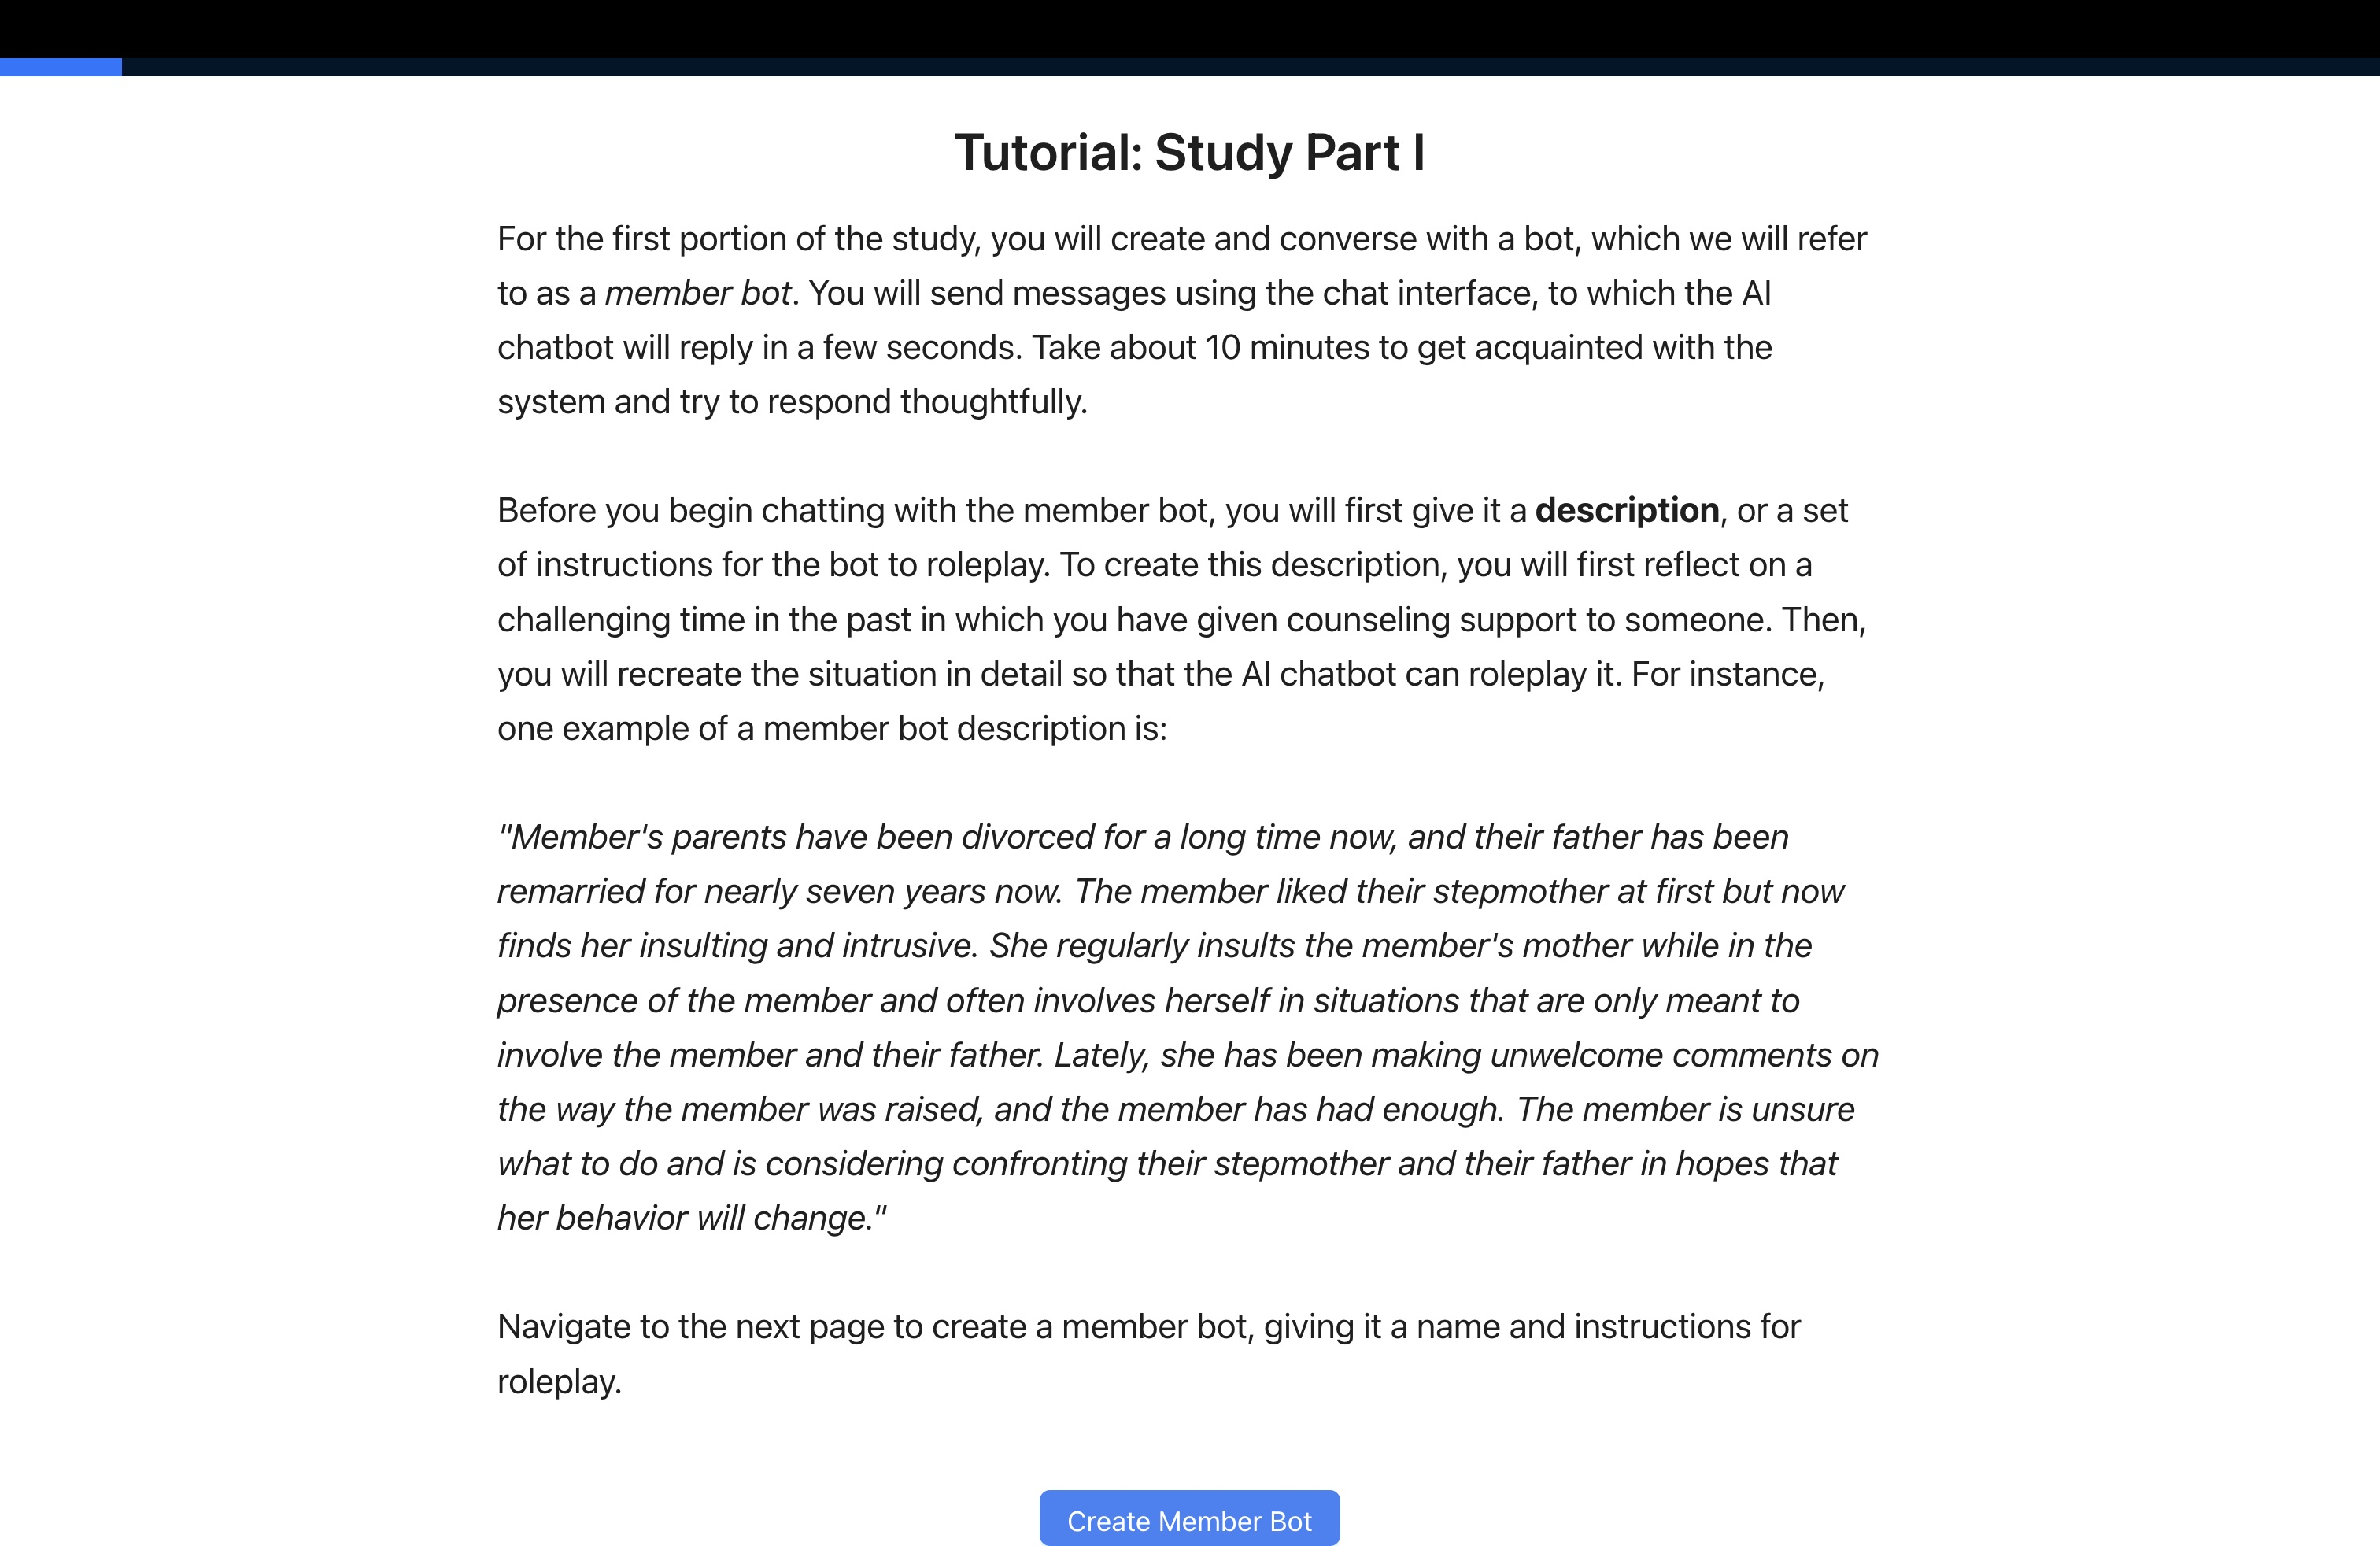
\includegraphics[width=\textwidth]{Study Screenshots/Screen2.jpeg}
    \caption{Part I instructions}
    \label{fig:screen2}
\end{figure*}

\begin{figure*}[ht]
    \centering
    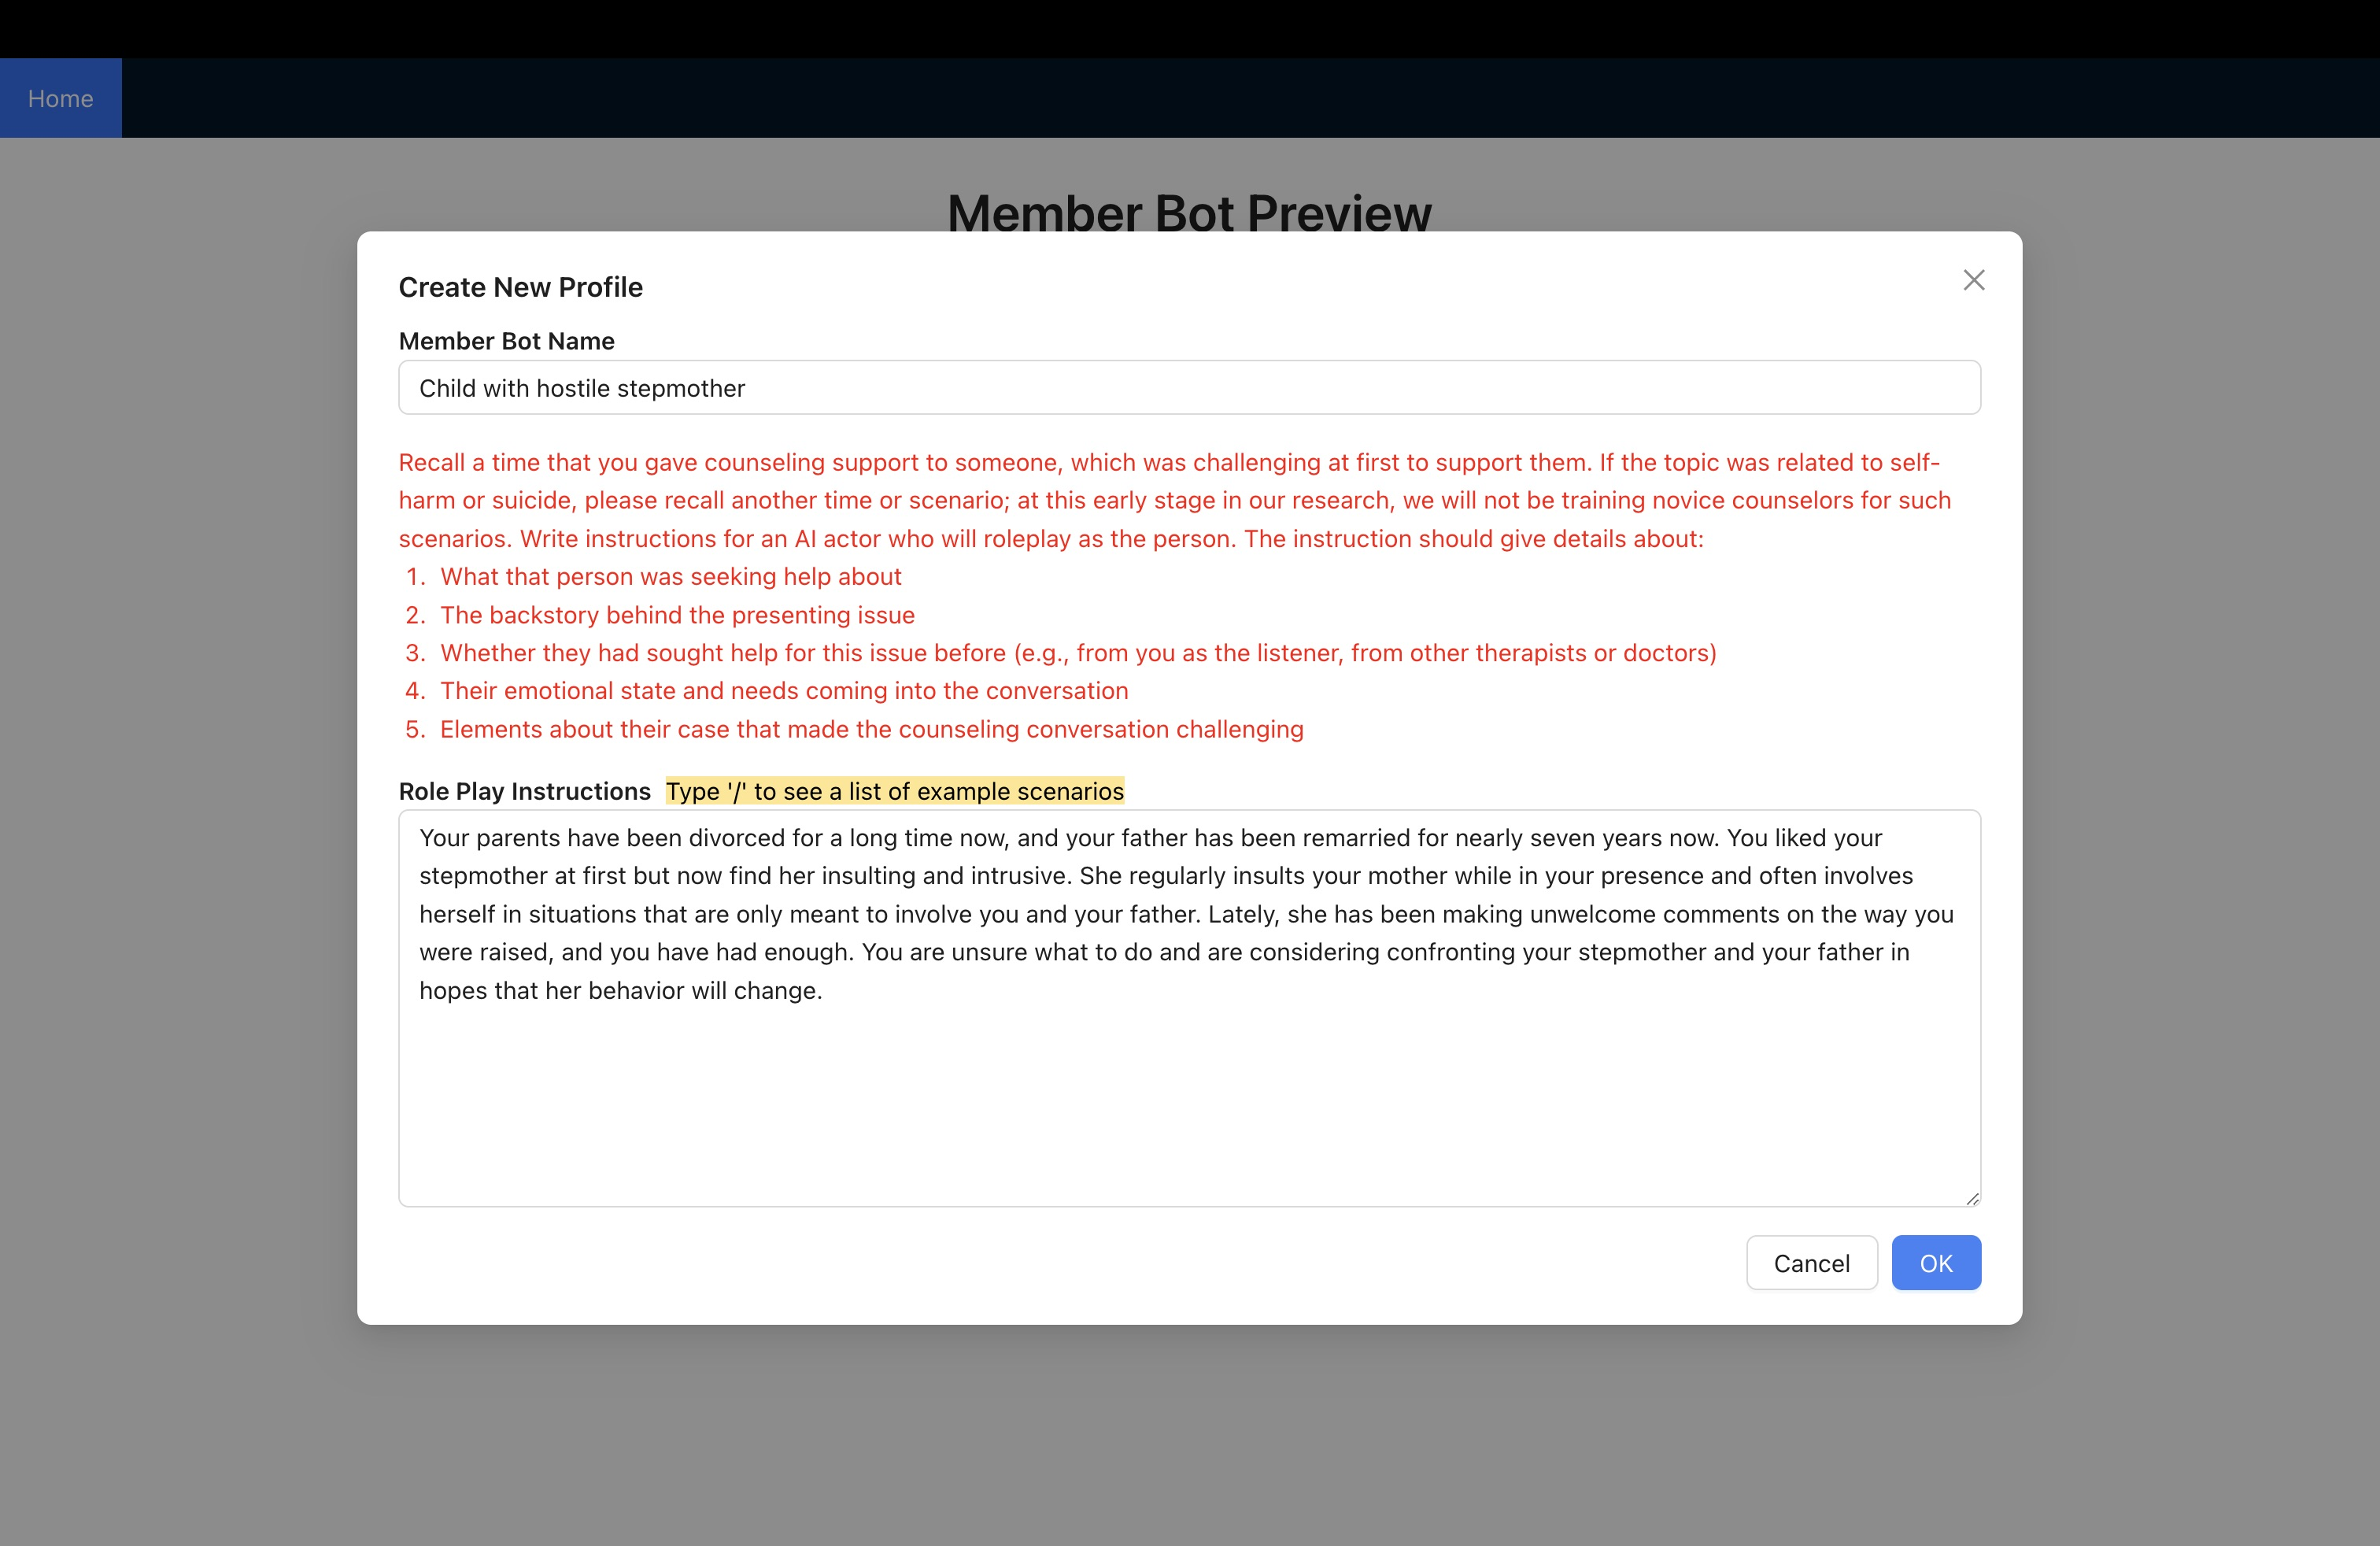
\includegraphics[width=\textwidth]{Study Screenshots/Screen3.jpeg}
    \caption{Creation of virtual patient}
    \label{fig:screen3}
\end{figure*}

\begin{figure*}[ht]
    \centering
    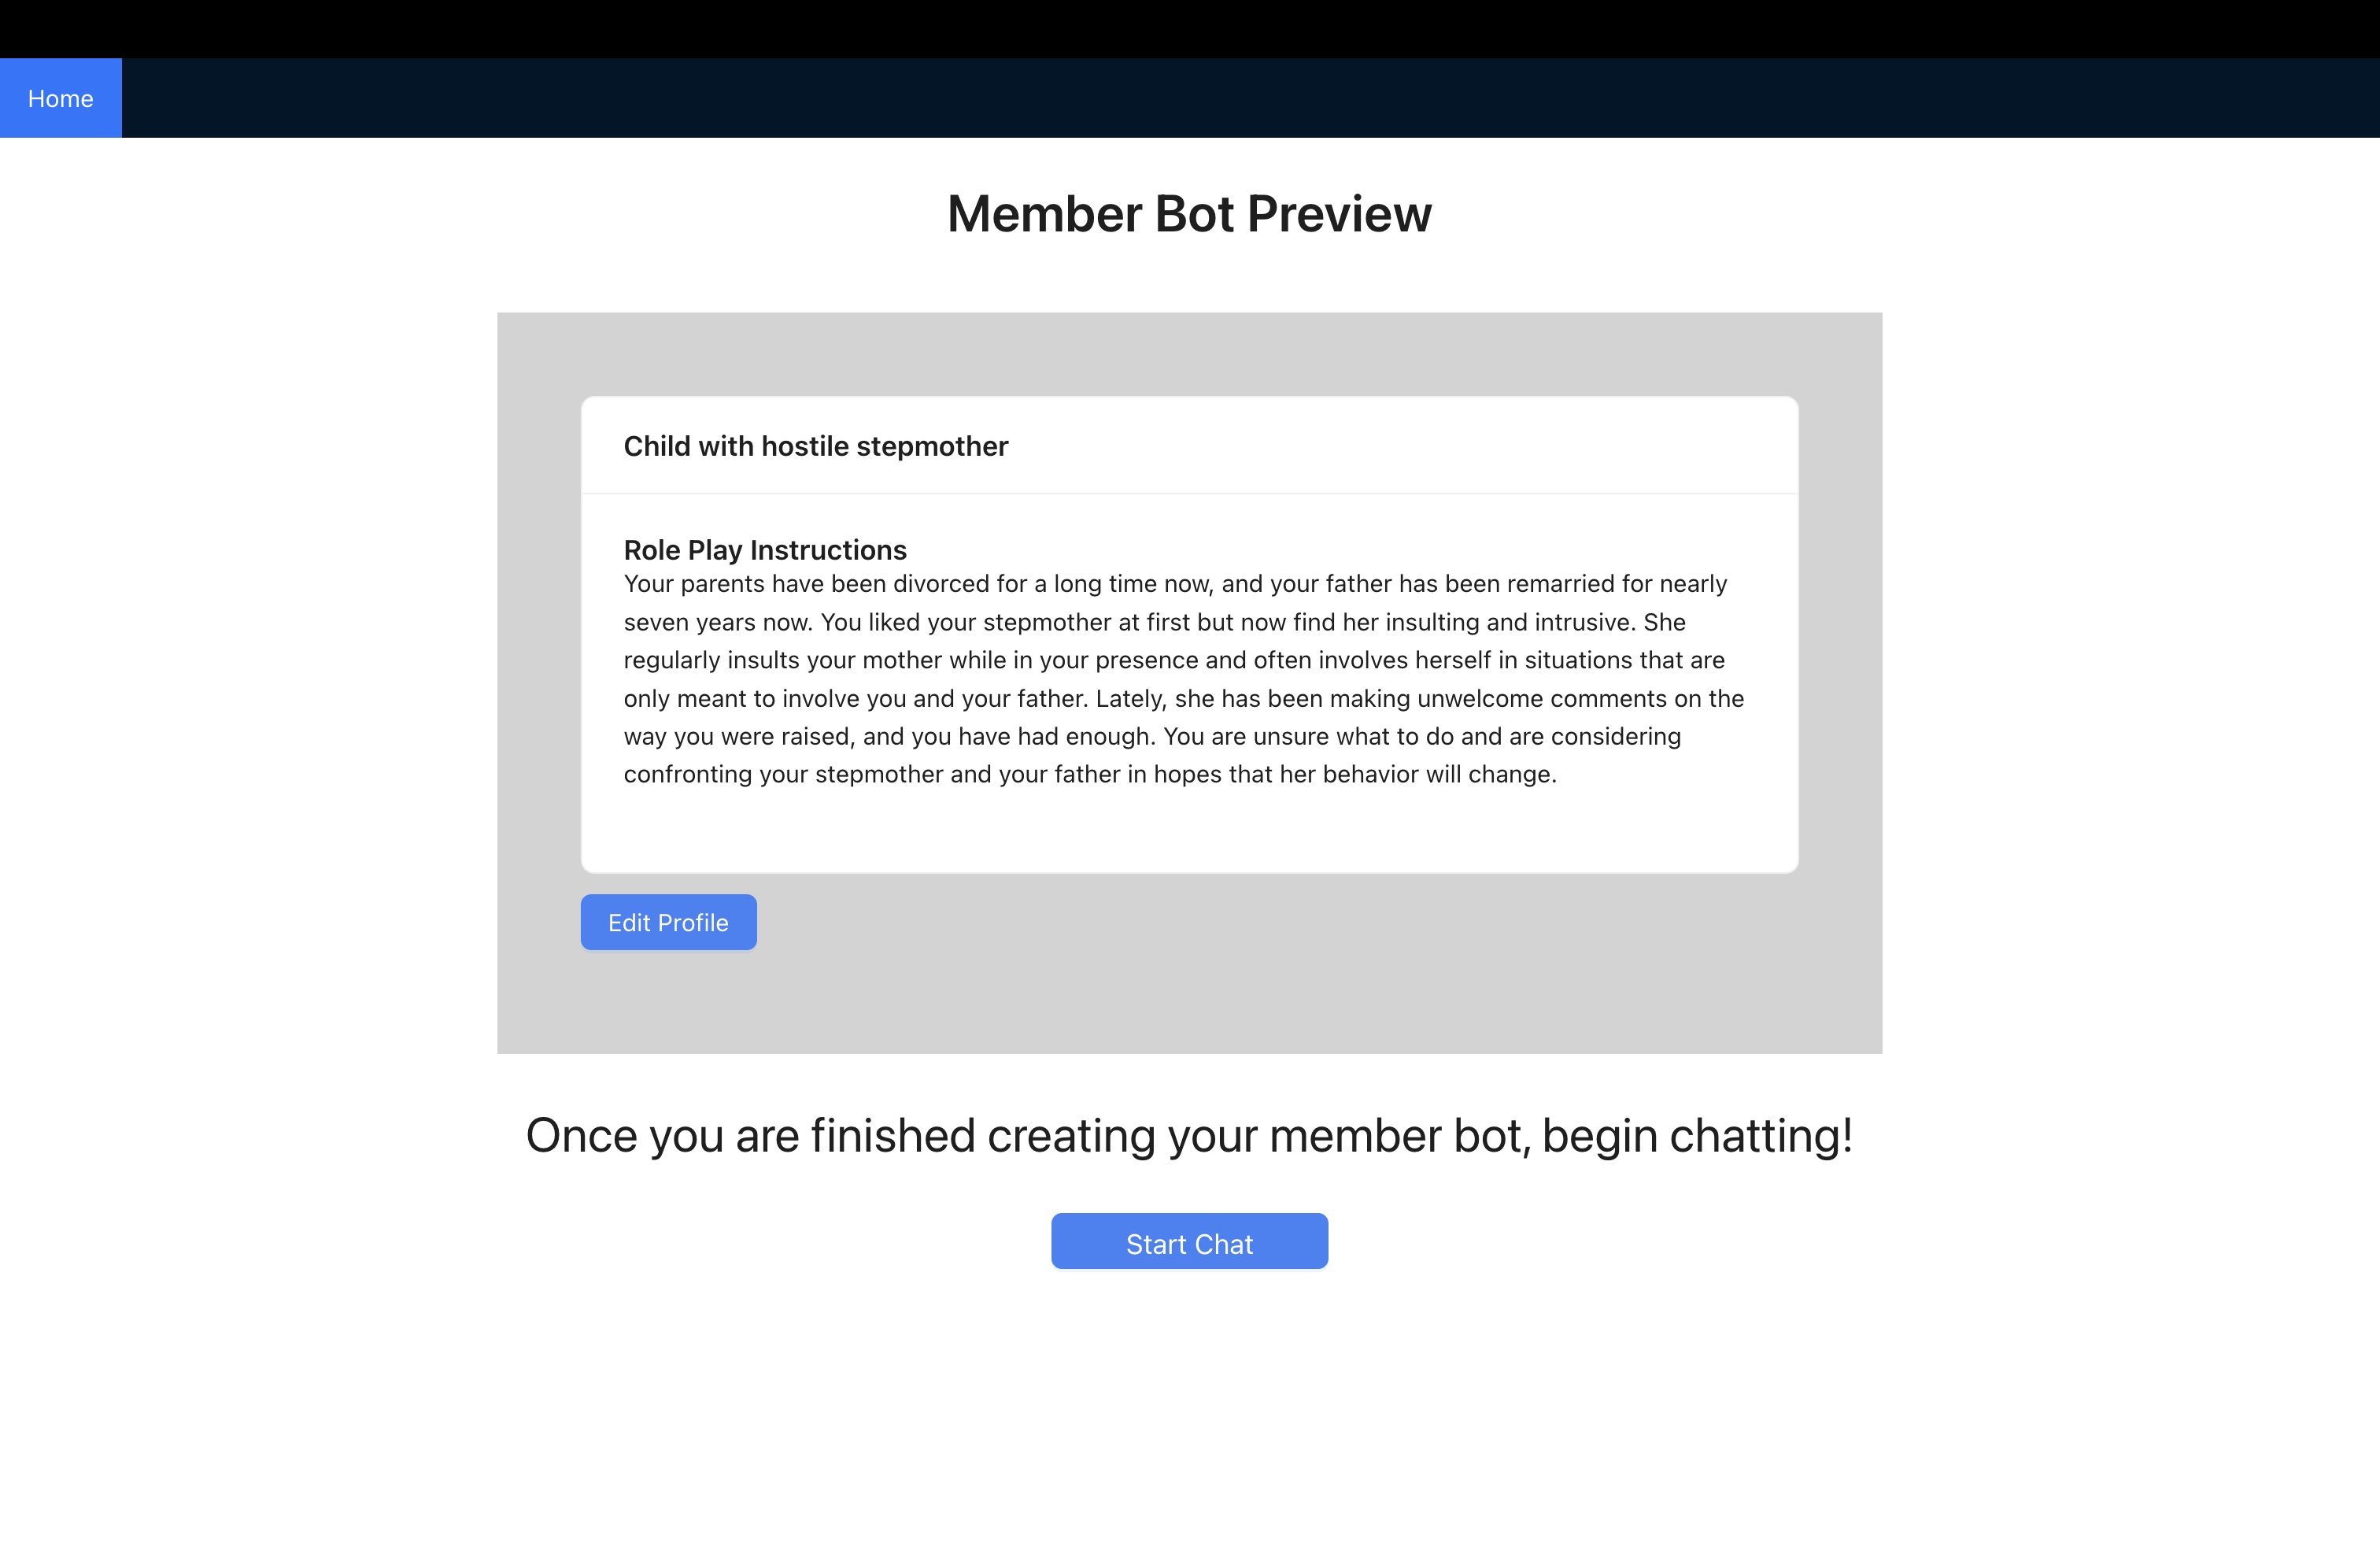
\includegraphics[width=\textwidth]{Study Screenshots/Screen4.jpeg}
    \caption{Virtual patient preview}
    \label{fig:screen4}
\end{figure*}

\begin{figure*}[ht]
    \centering
    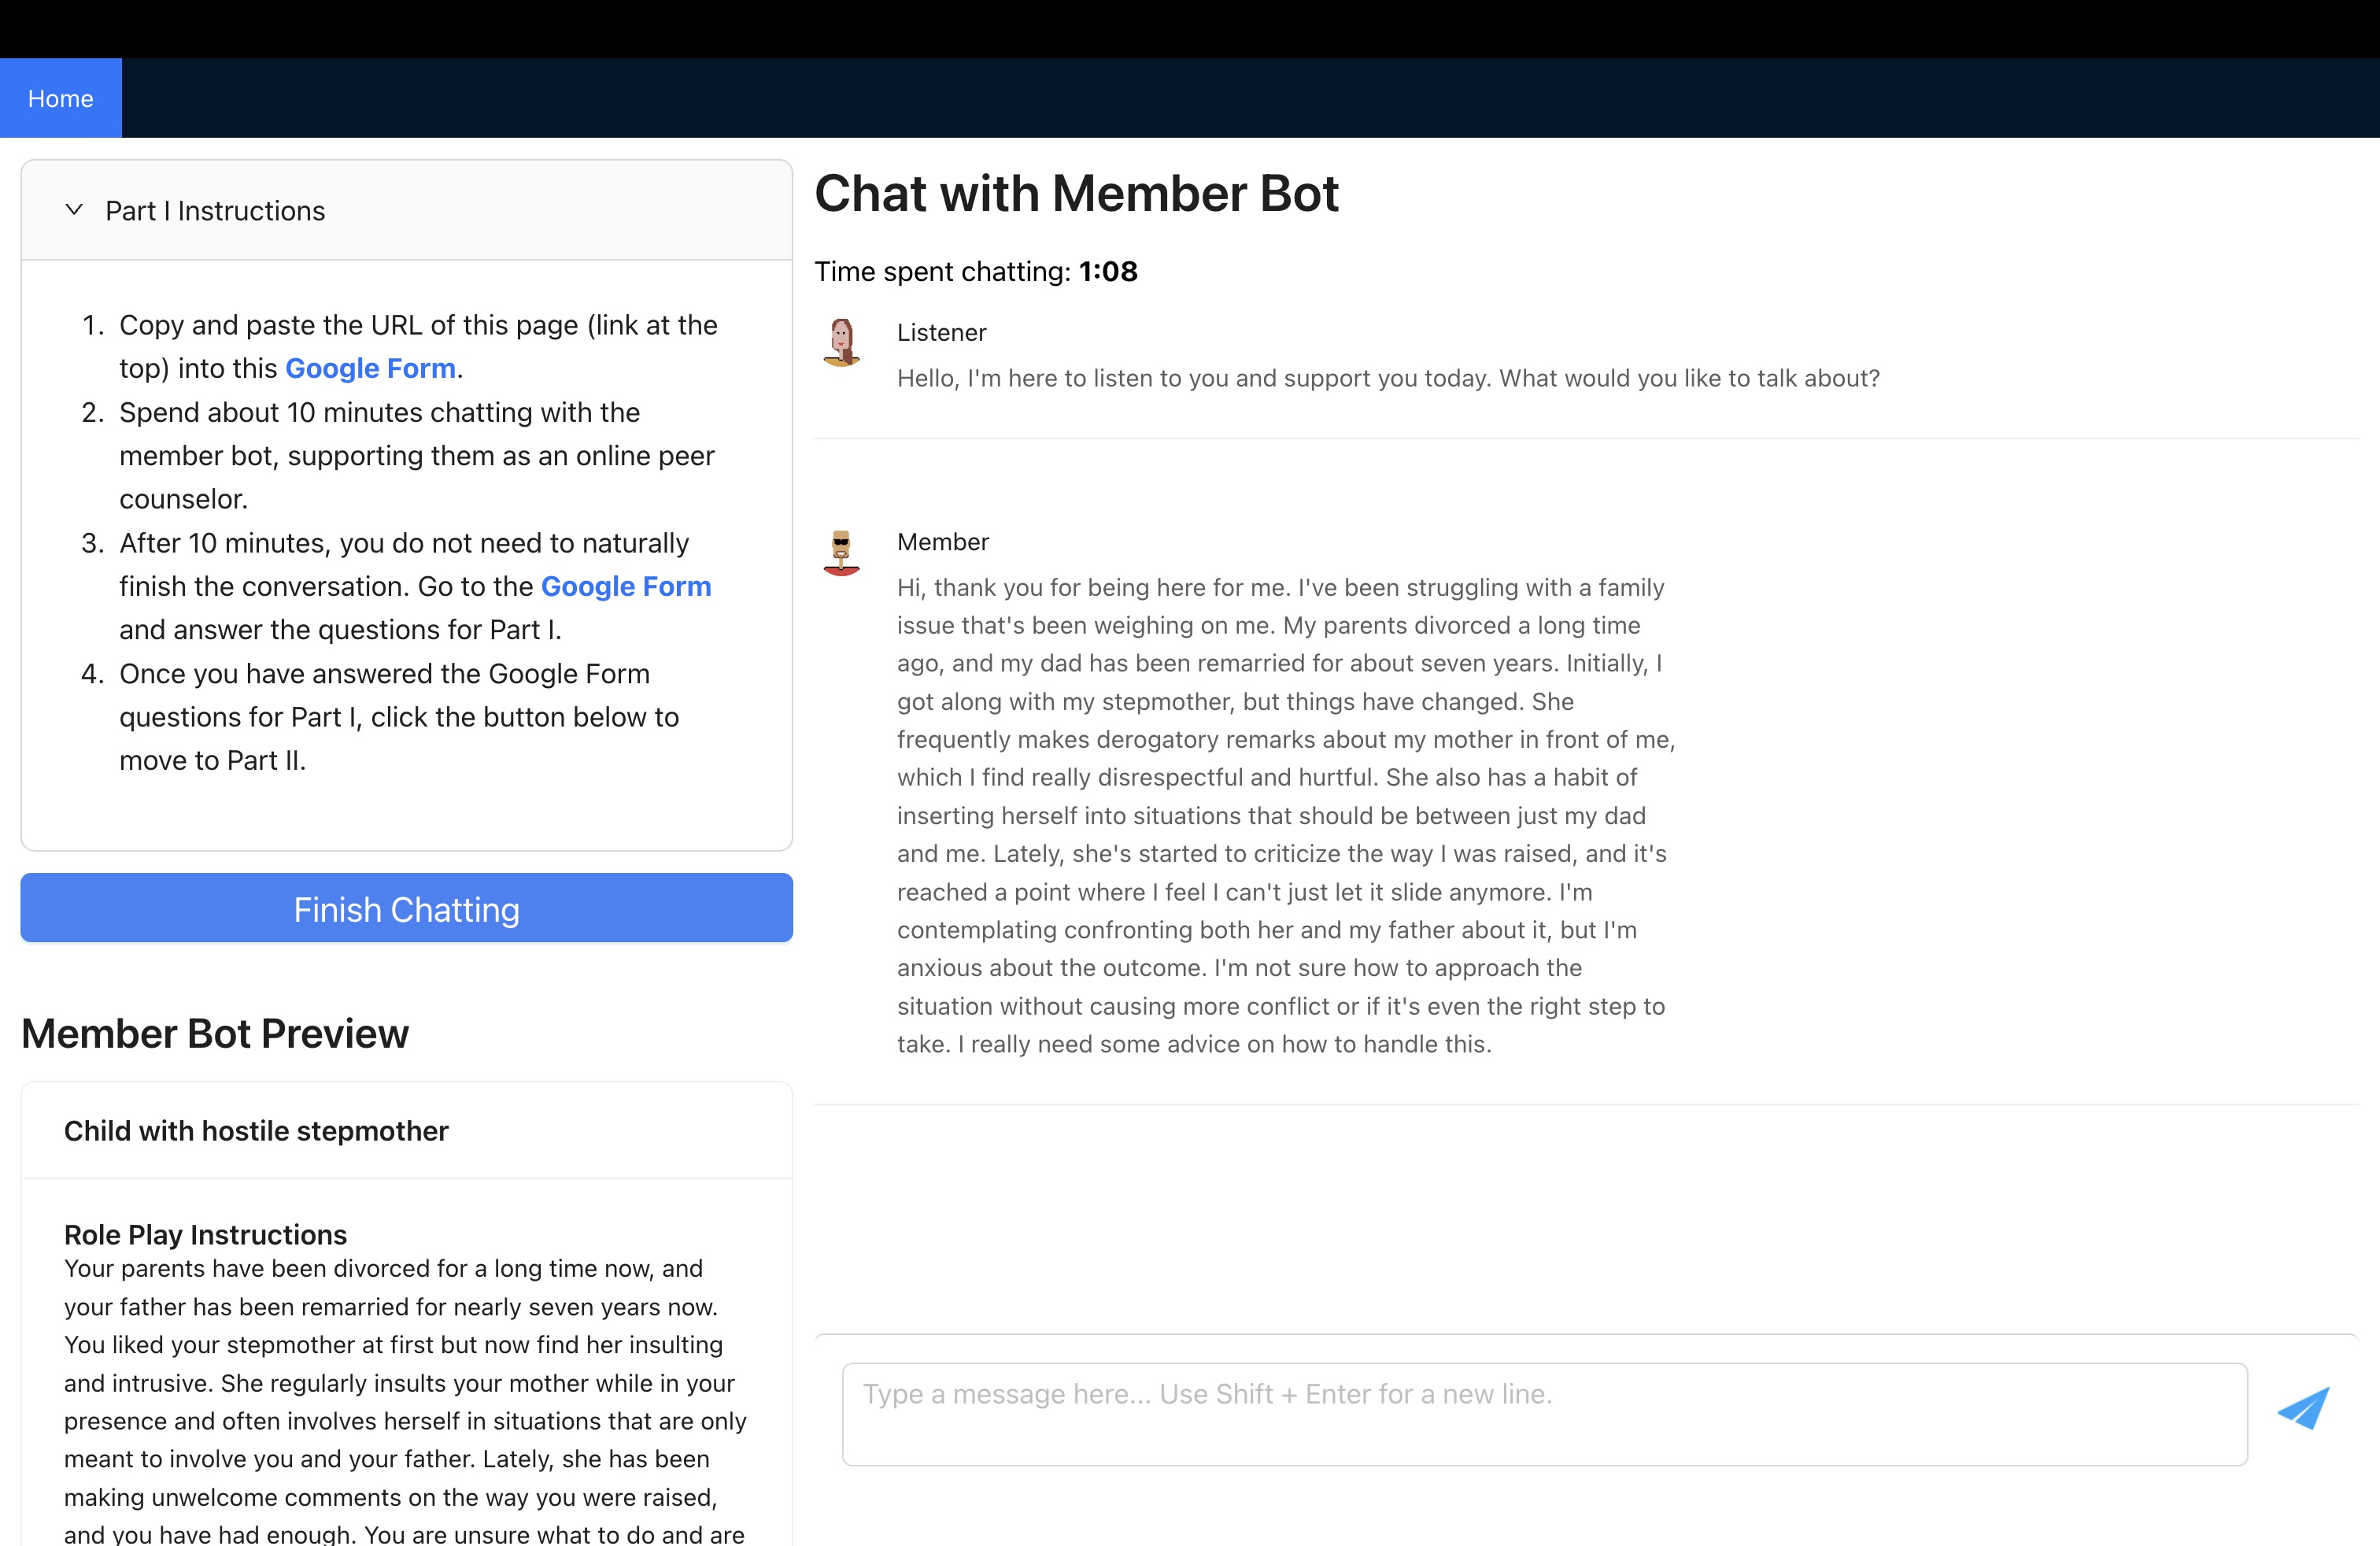
\includegraphics[width=\textwidth]{Study Screenshots/Screen5.jpeg}
    \caption{Part I chat with \textit{Scenario-Only} virtual patient}
    \label{fig:screen5}
\end{figure*}

\begin{figure*}[ht]
    \centering
    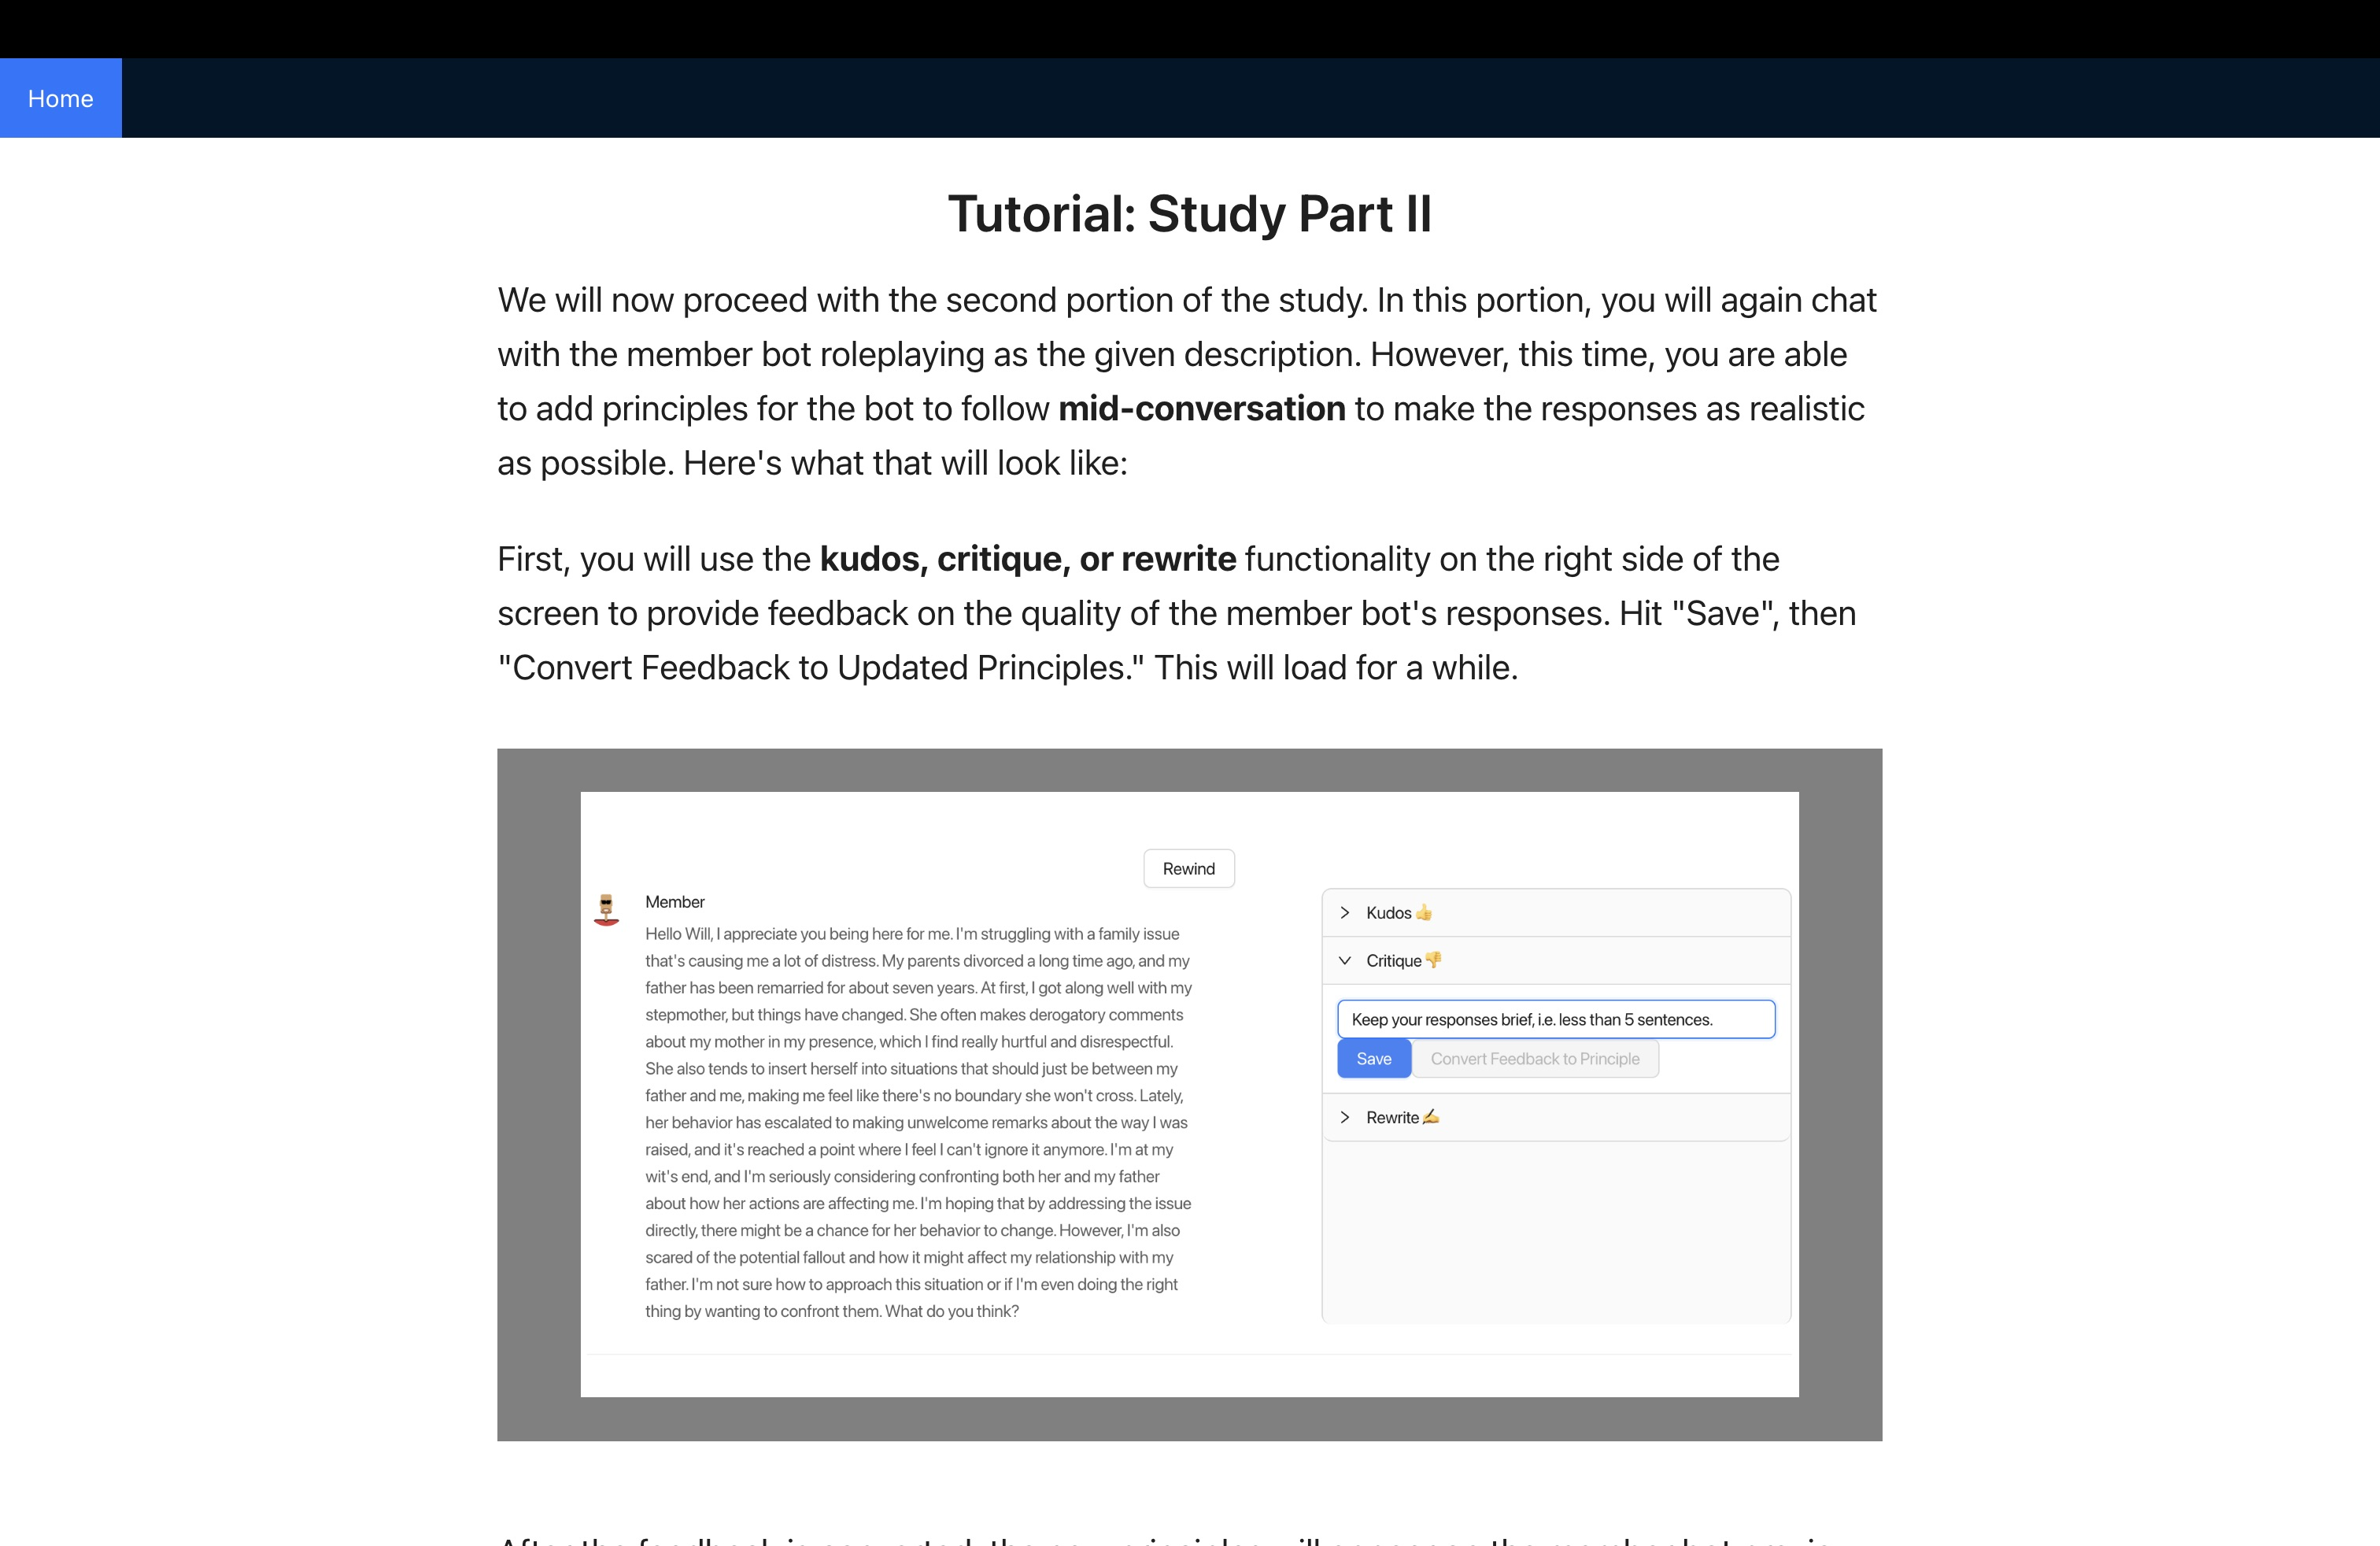
\includegraphics[width=\textwidth]{Study Screenshots/Screen6.jpeg}
    \caption{Part II instructions}
    \label{fig:screen6}
\end{figure*}

\begin{figure*}[ht]
    \centering
    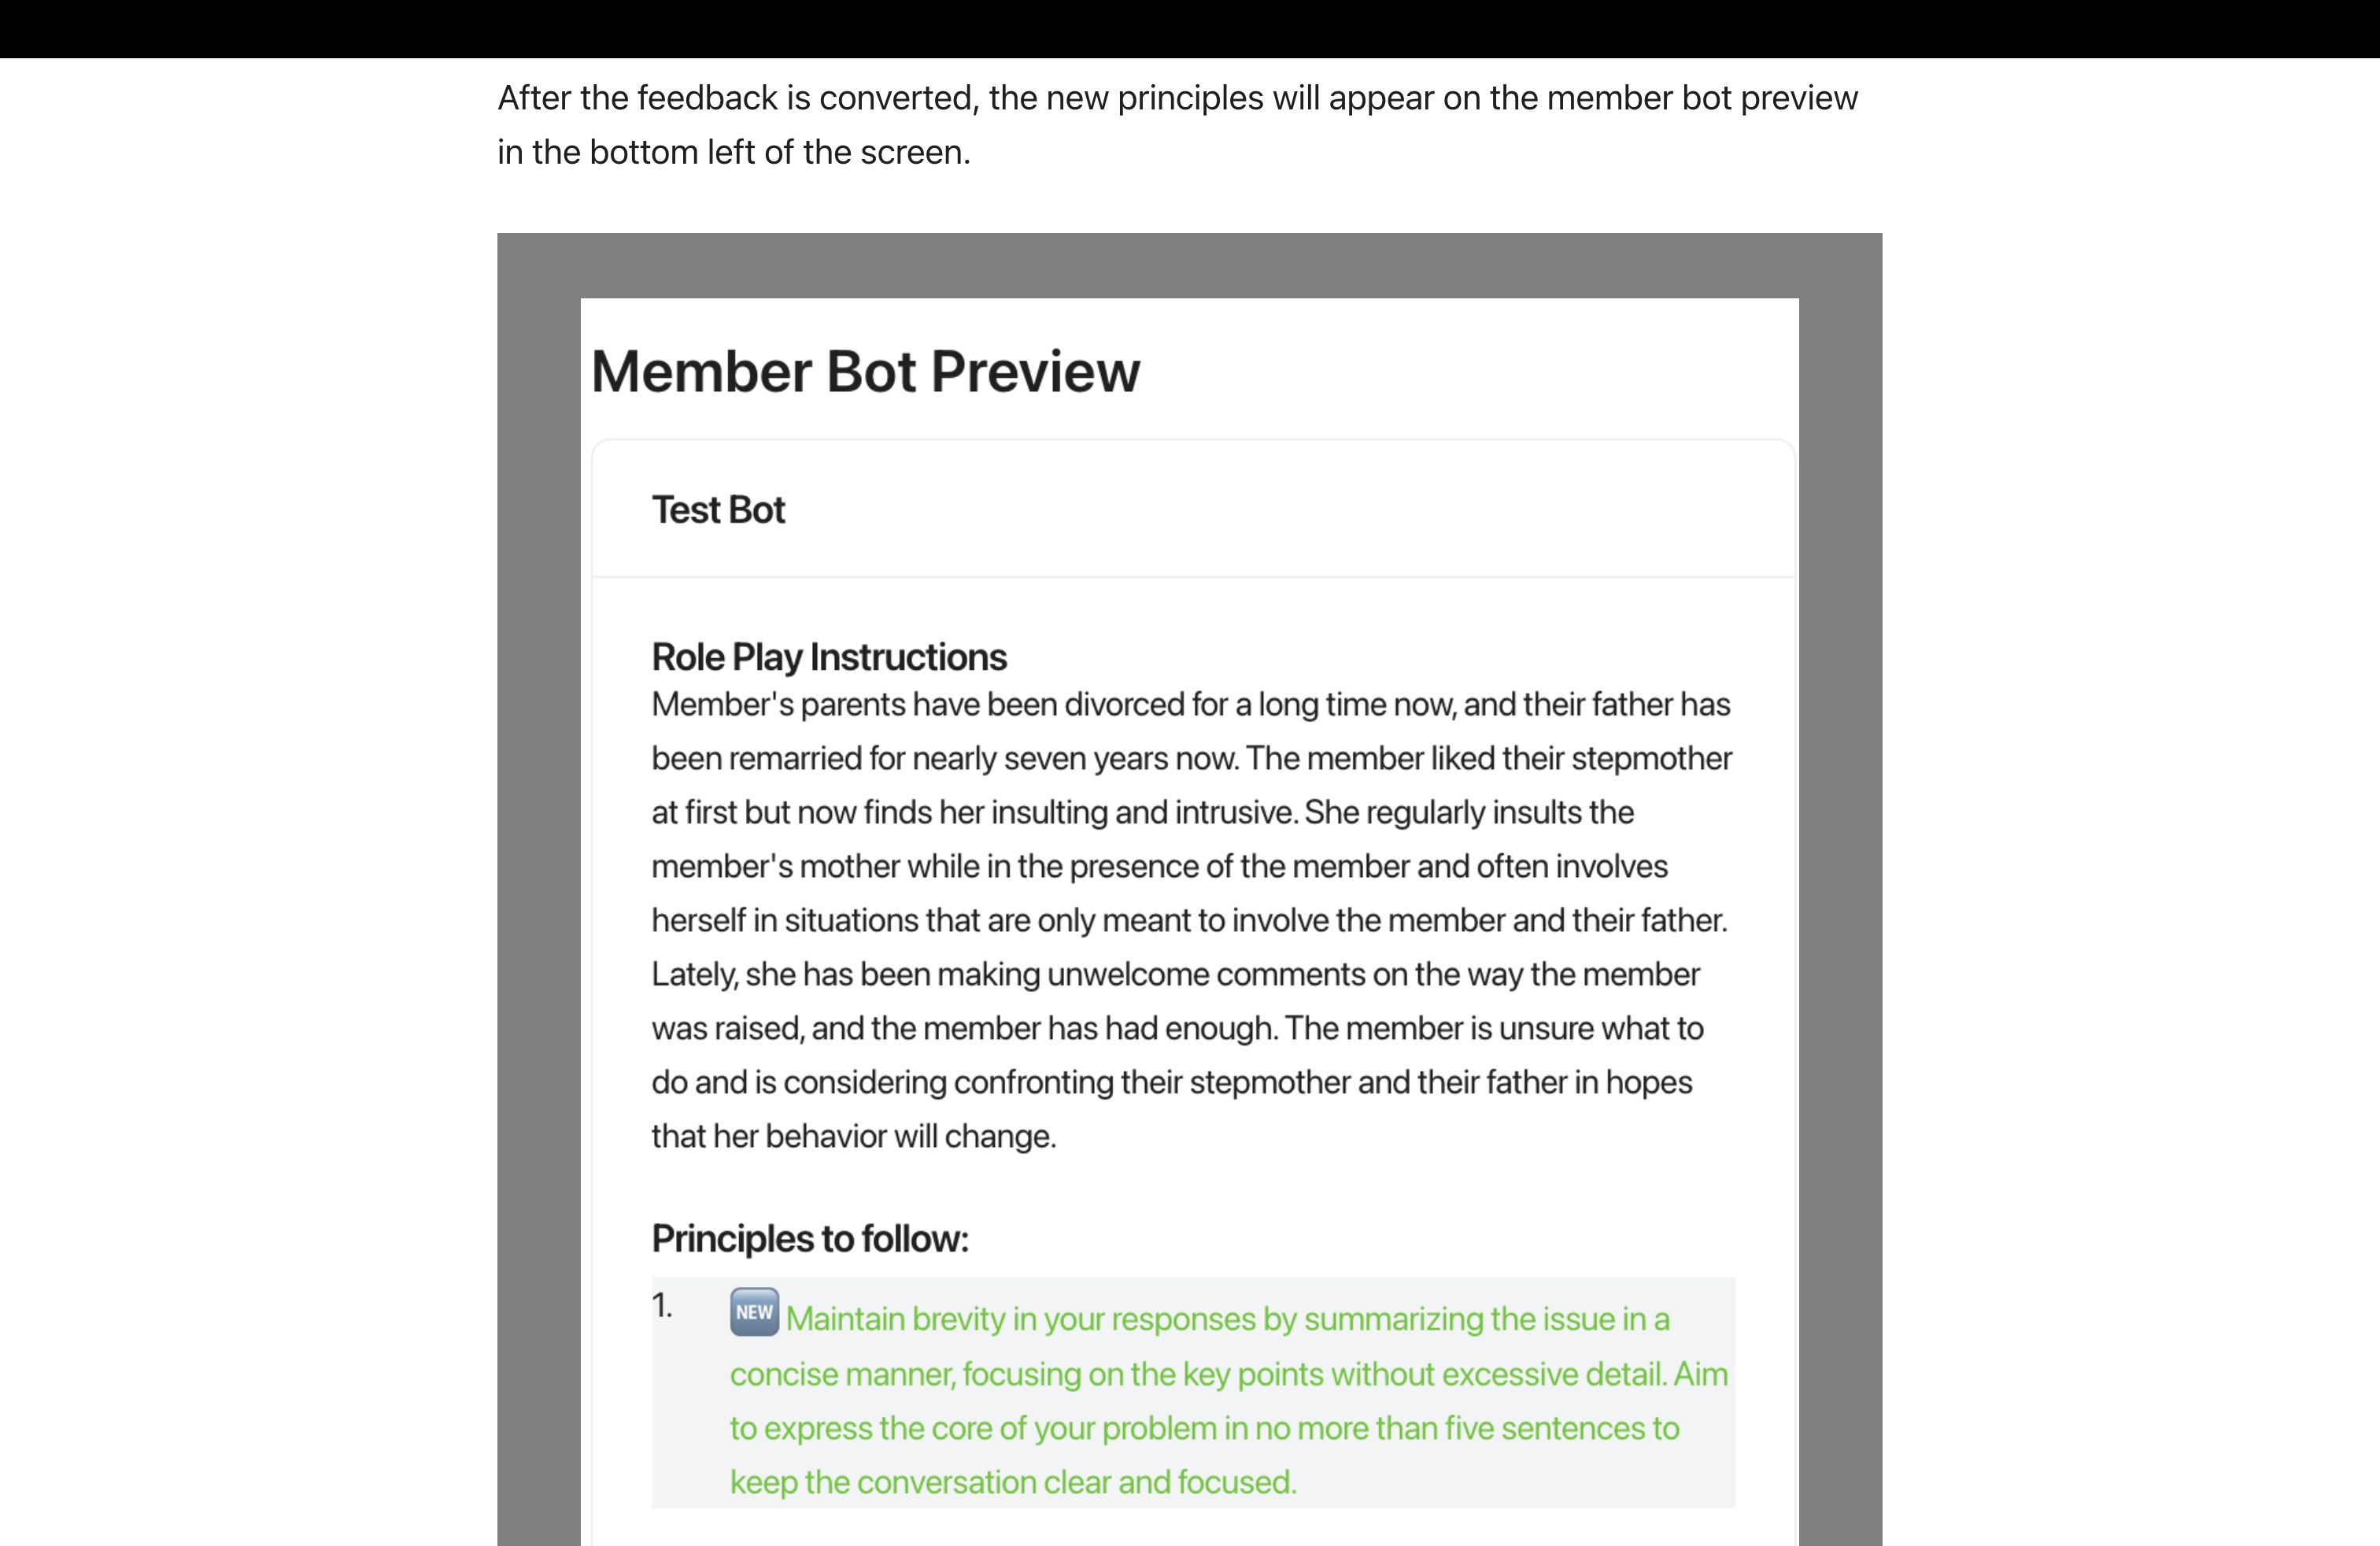
\includegraphics[width=\textwidth]{Study Screenshots/Screen7.jpeg}
    \caption{Part II instructions (continued)}
    \label{fig:screen7}
\end{figure*}

\begin{figure*}[ht]
    \centering
    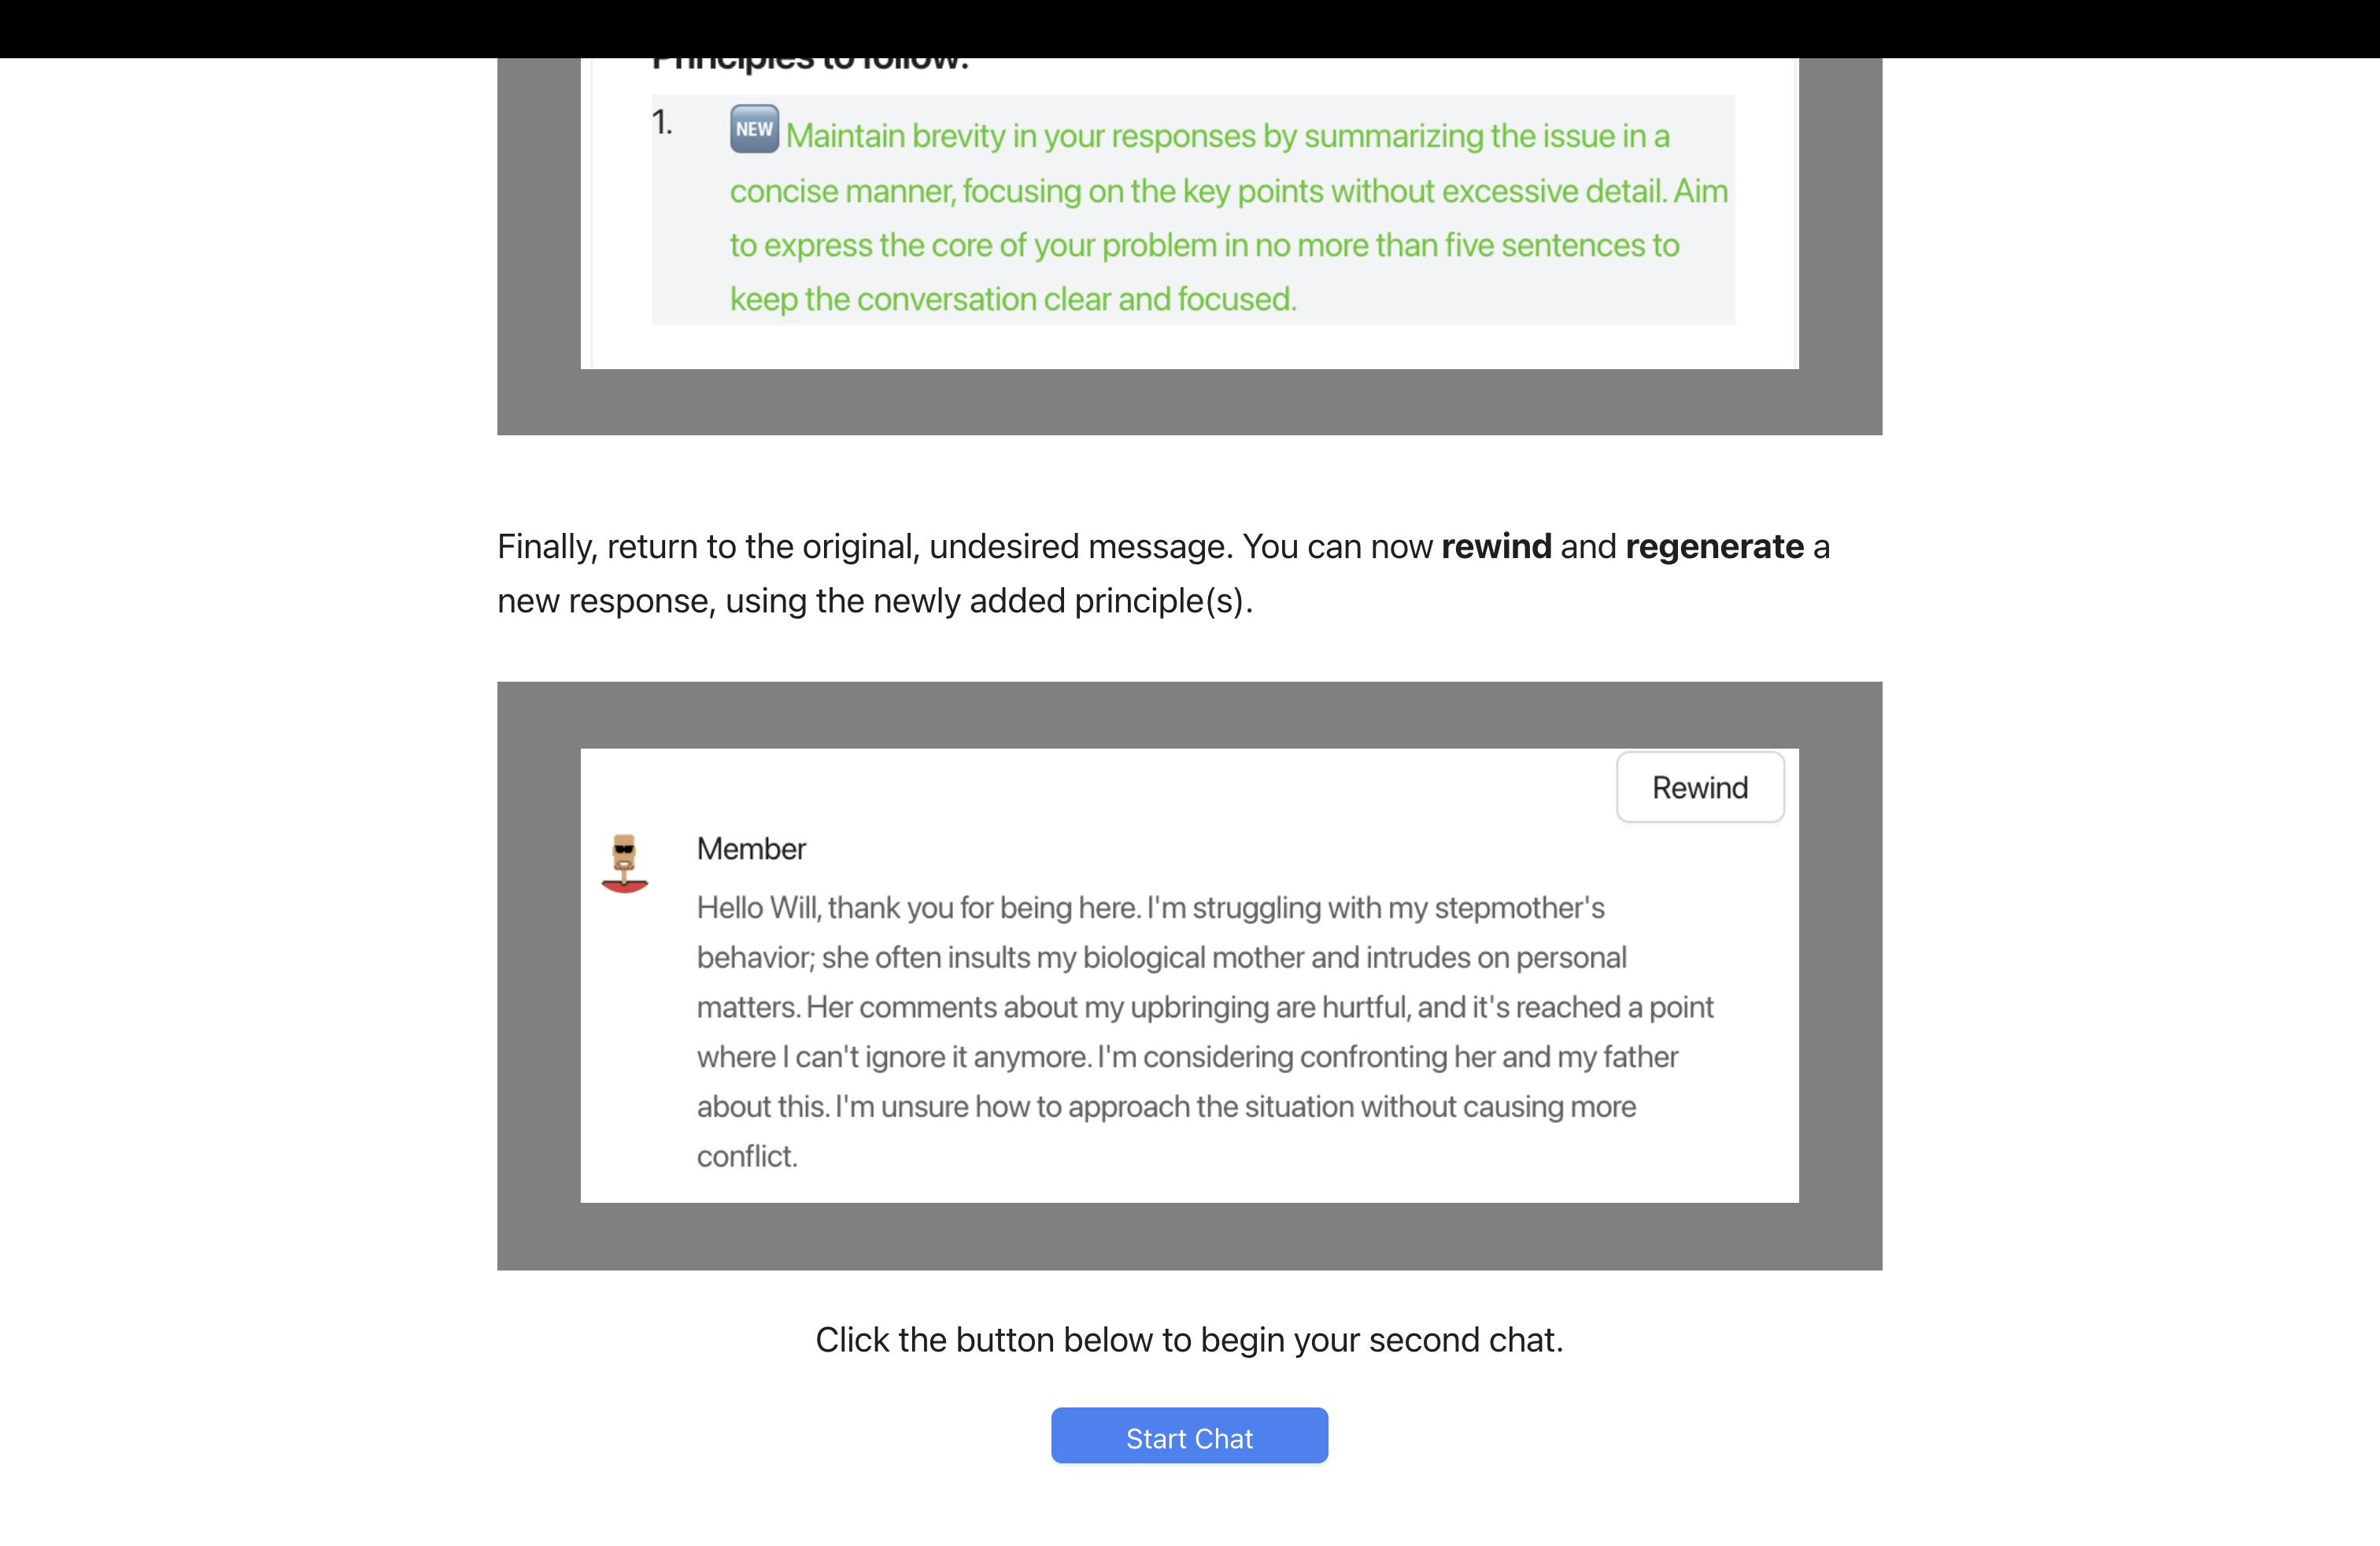
\includegraphics[width=\textwidth]{Study Screenshots/Screen8.jpeg}
    \caption{Part II instructions (continued)}
    \label{fig:screen8}
\end{figure*}

\begin{figure*}[ht]
    \centering
    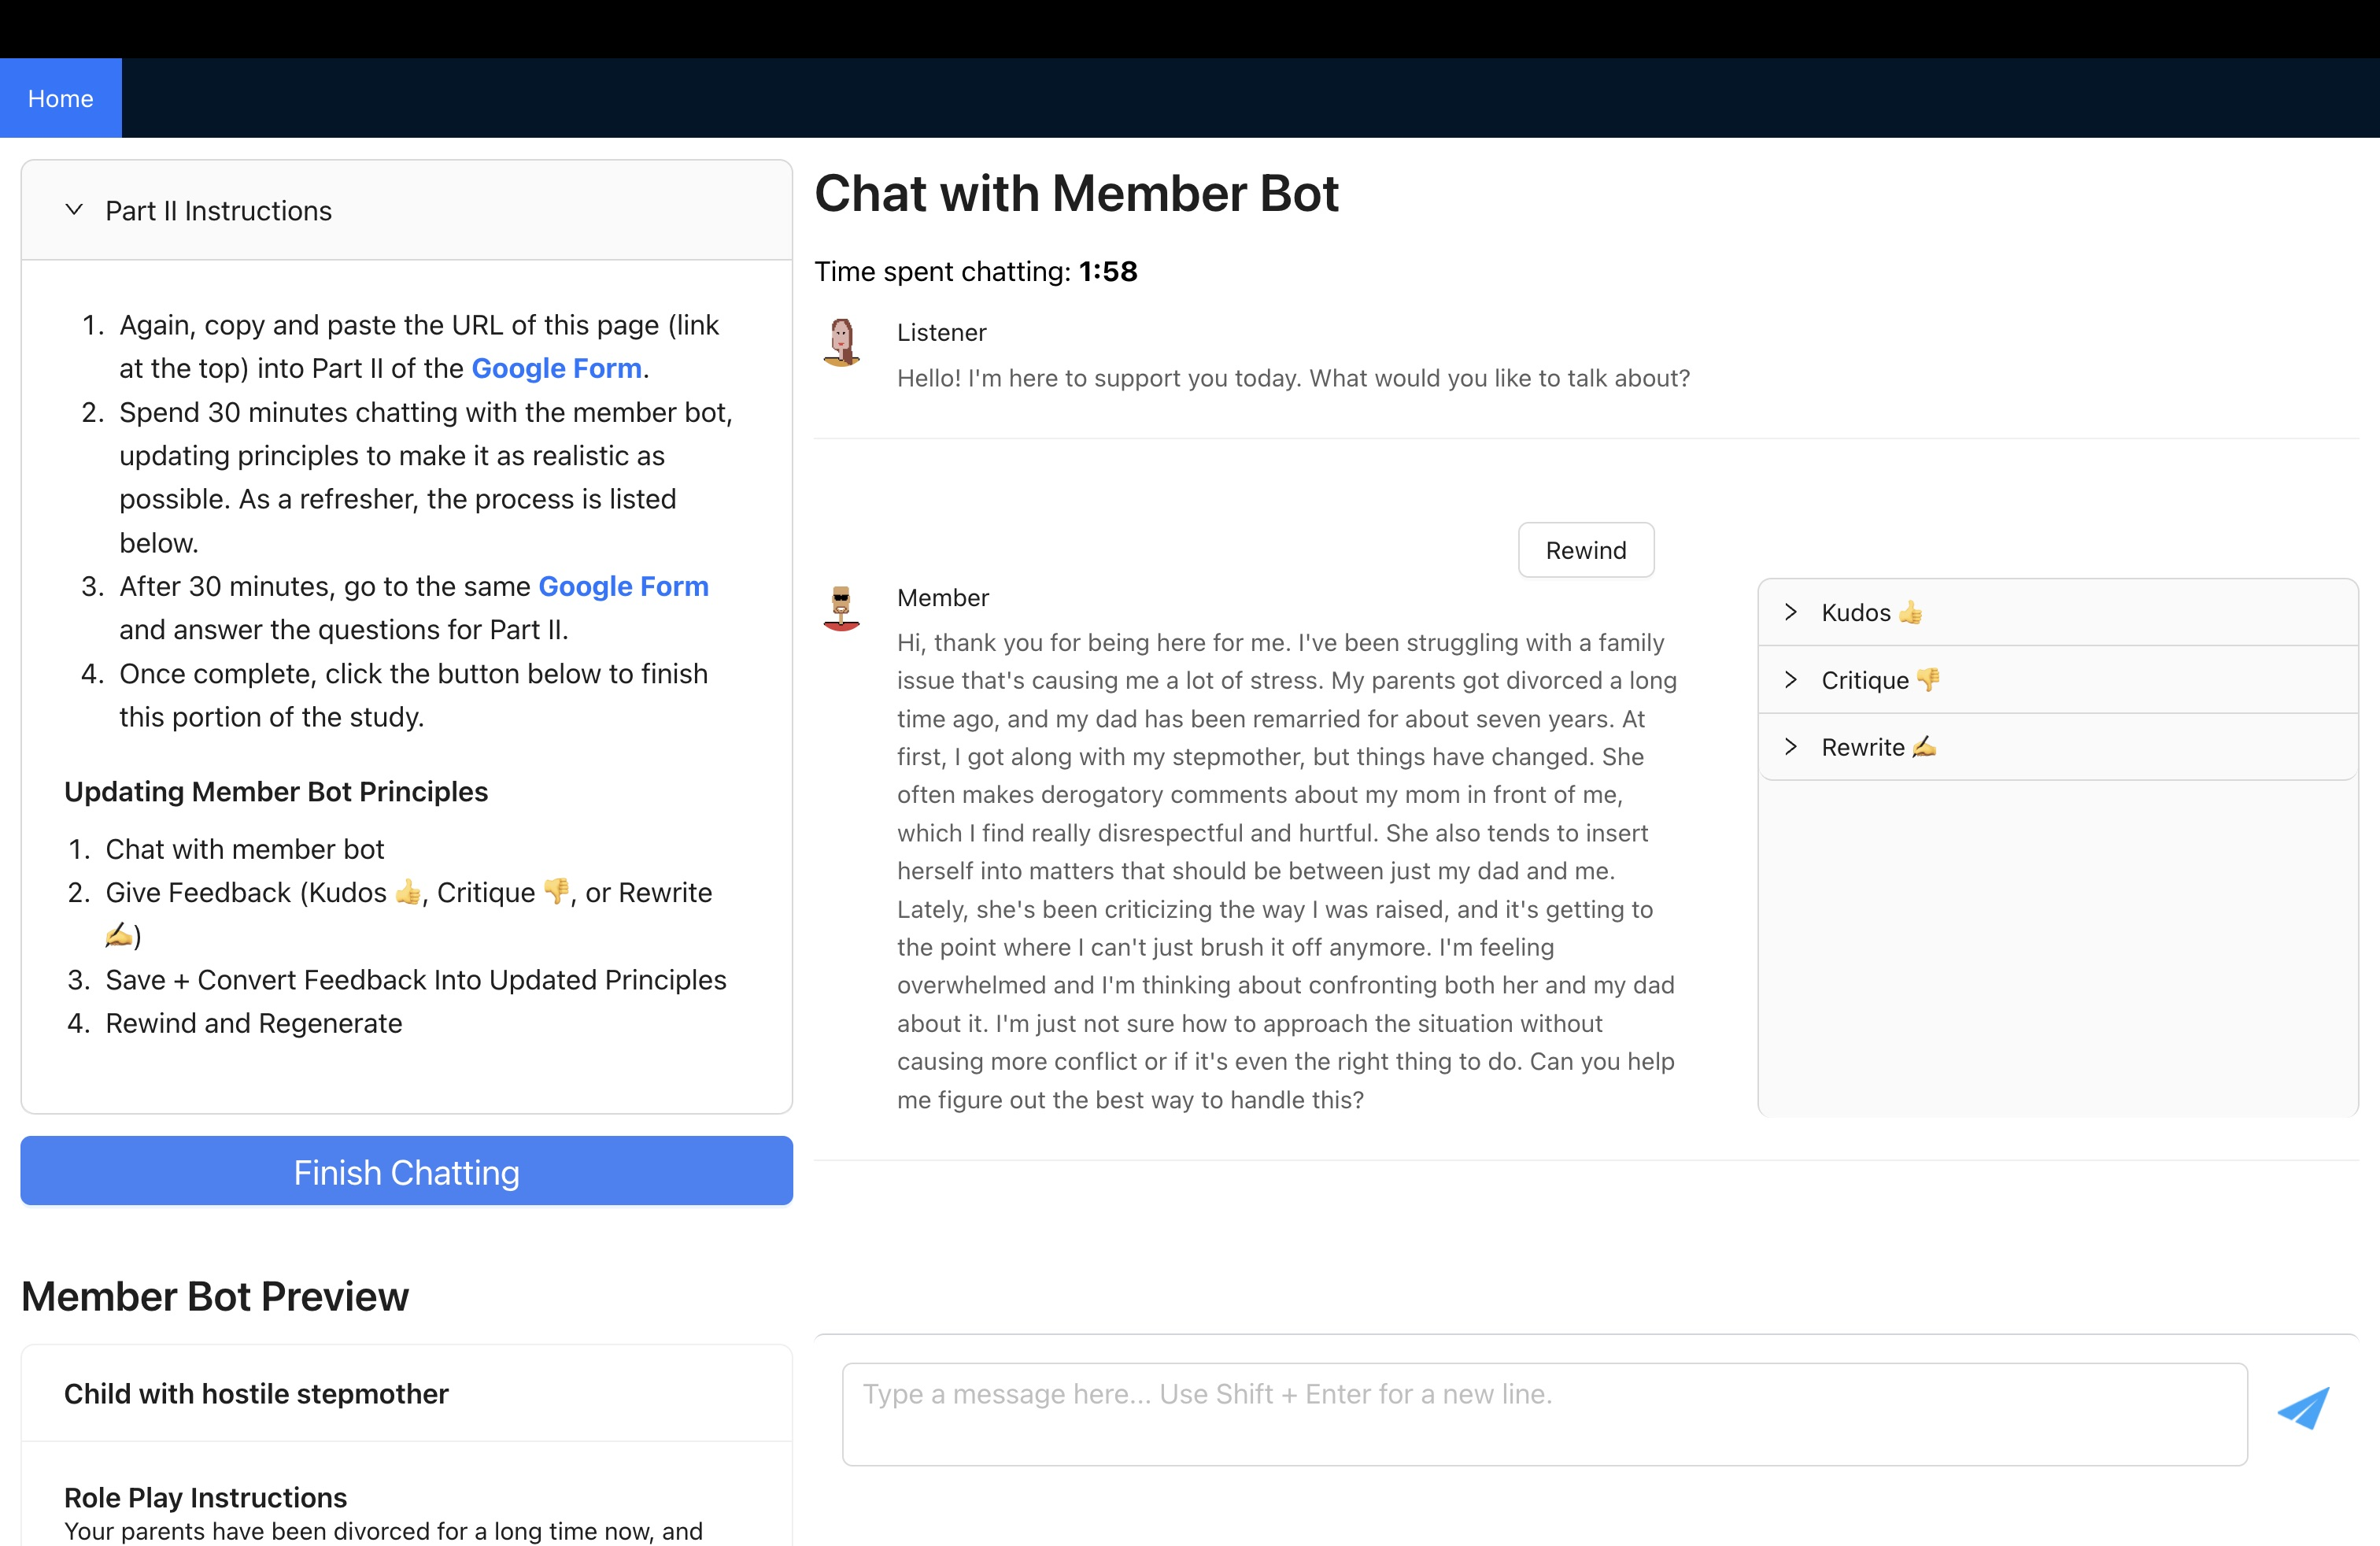
\includegraphics[width=\textwidth]{Study Screenshots/Screen10.jpeg}
    \caption{Part II chat with \textit{Scenario+Expert-Principles} bot}
    \label{fig:screen10}
\end{figure*}

\begin{figure*}[ht]
    \centering
    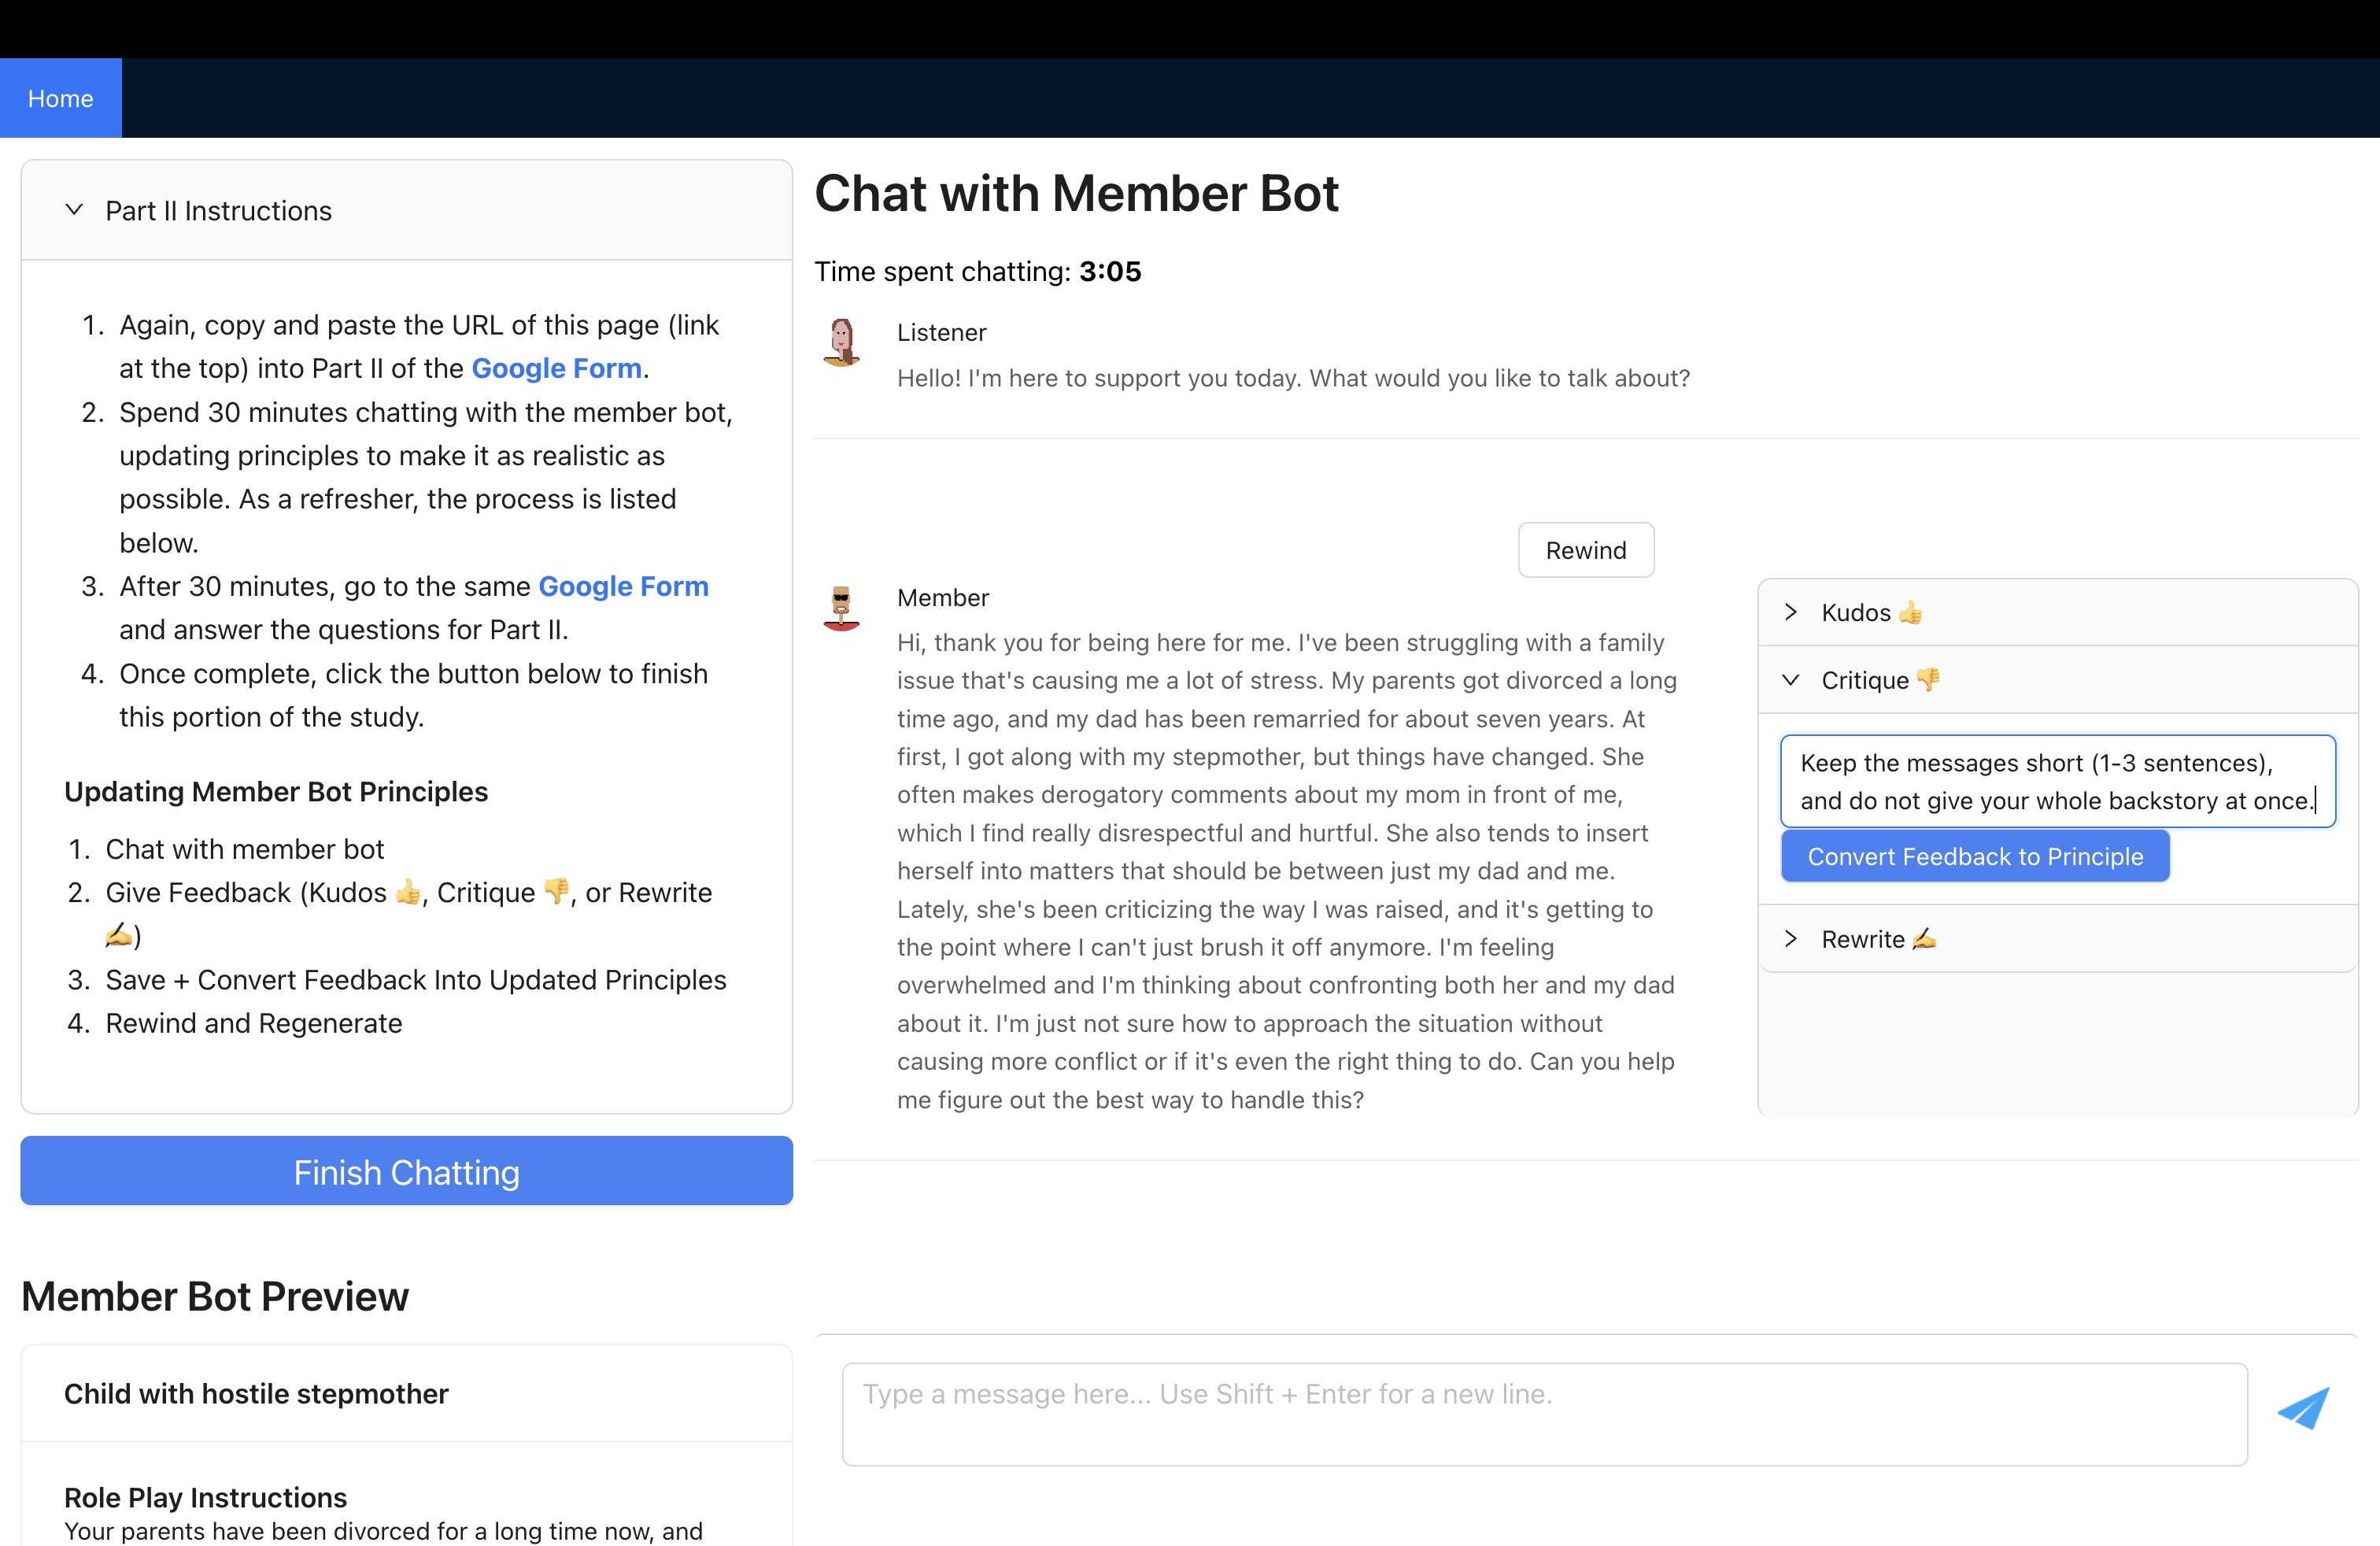
\includegraphics[width=\textwidth]{Study Screenshots/Screen11.jpeg}
    \caption{Using kudos/critique/rewrite to give feedback}
    \label{fig:screen11}
\end{figure*}

\begin{figure*}[ht]
    \centering
    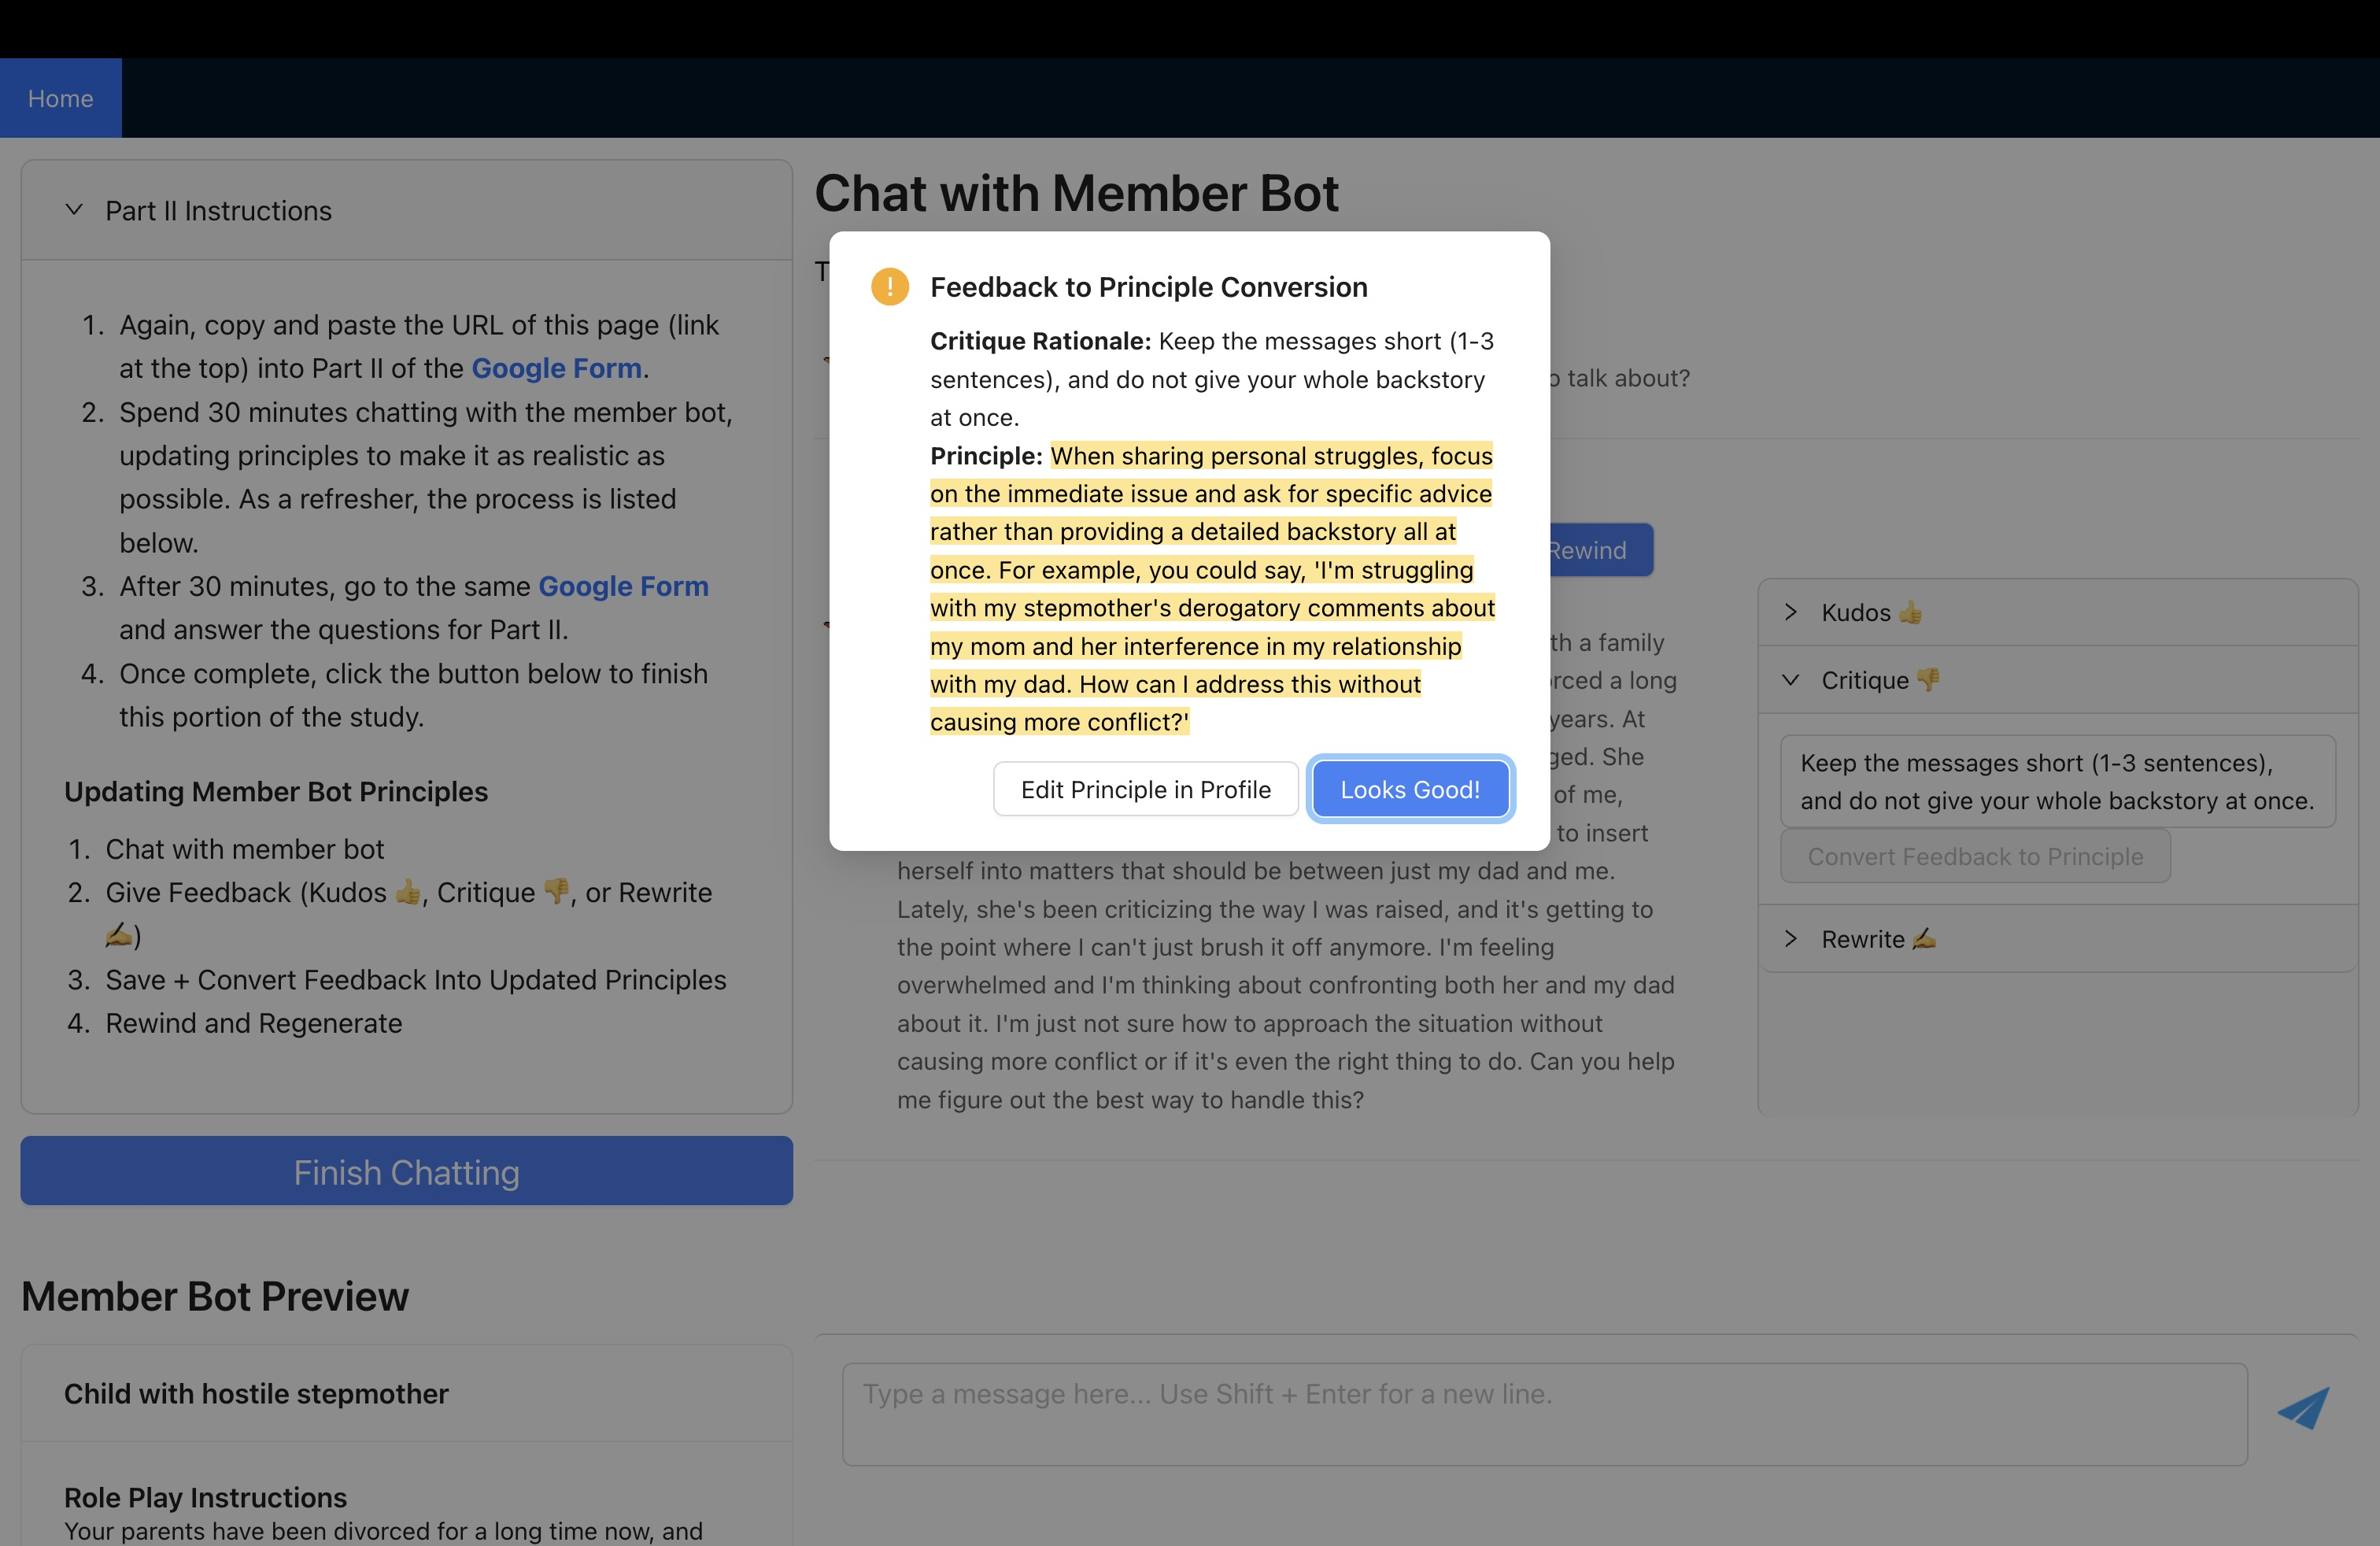
\includegraphics[width=\textwidth]{Study Screenshots/Screen12.jpeg}
    \caption{Feedback converted into principle}
    \label{fig:screen12}
\end{figure*}

\begin{figure*}[ht]
    \centering
    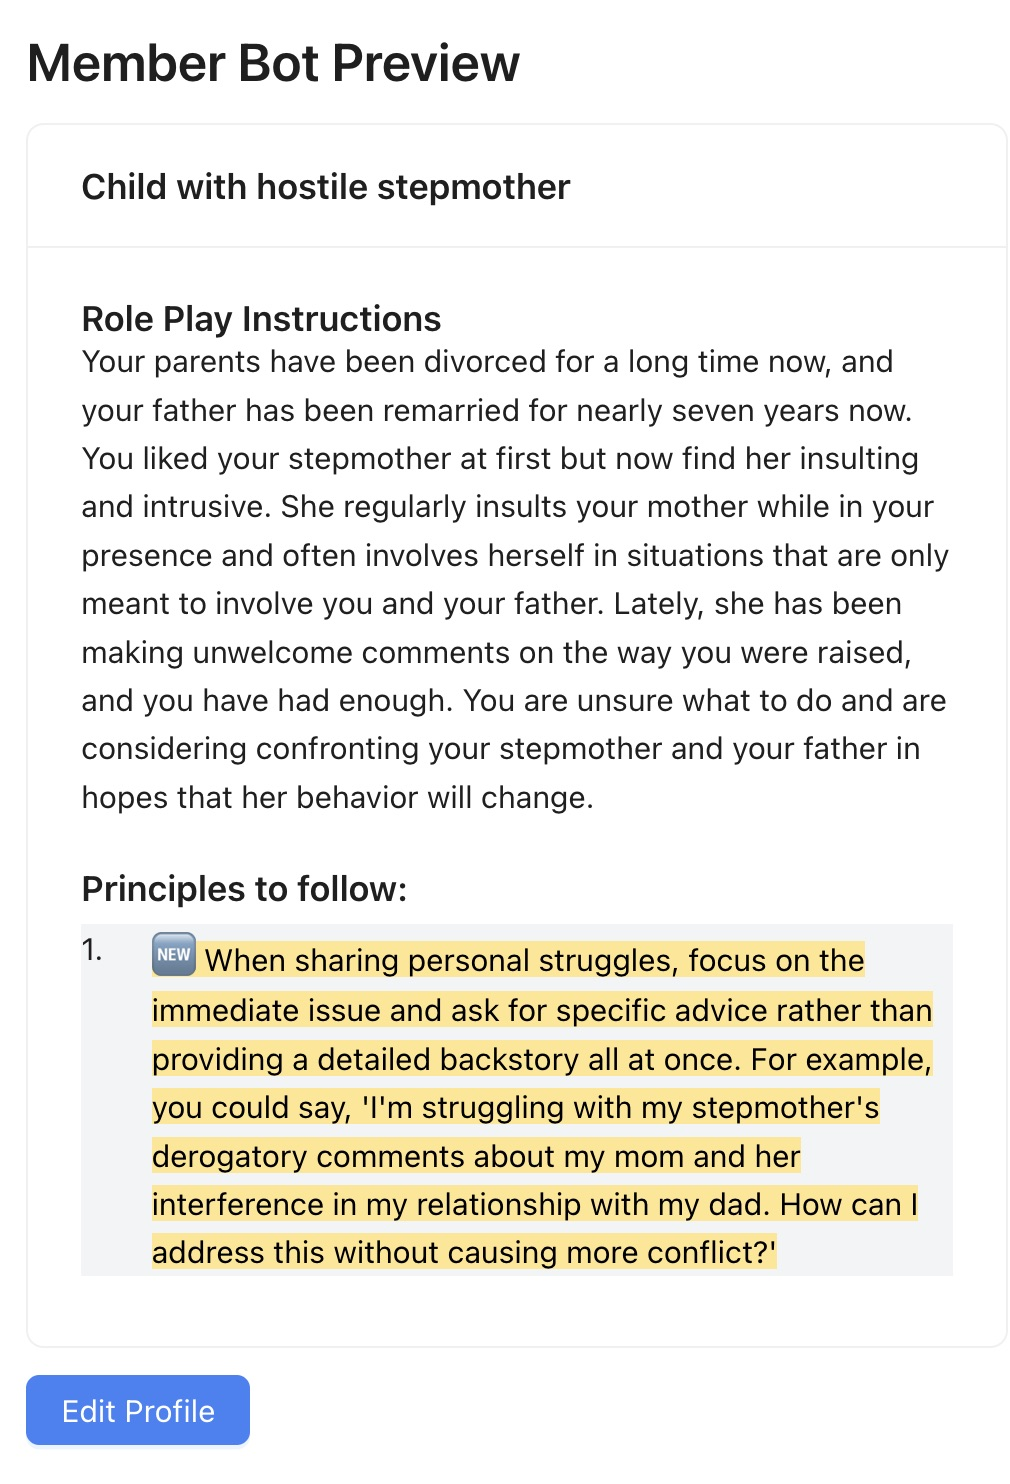
\includegraphics[width=\textwidth]{Study Screenshots/Screen13.jpeg}
    \caption{New principle incorporated into virtual patient}
    \label{fig:screen13}
\end{figure*}

\begin{figure*}[ht]
    \centering
    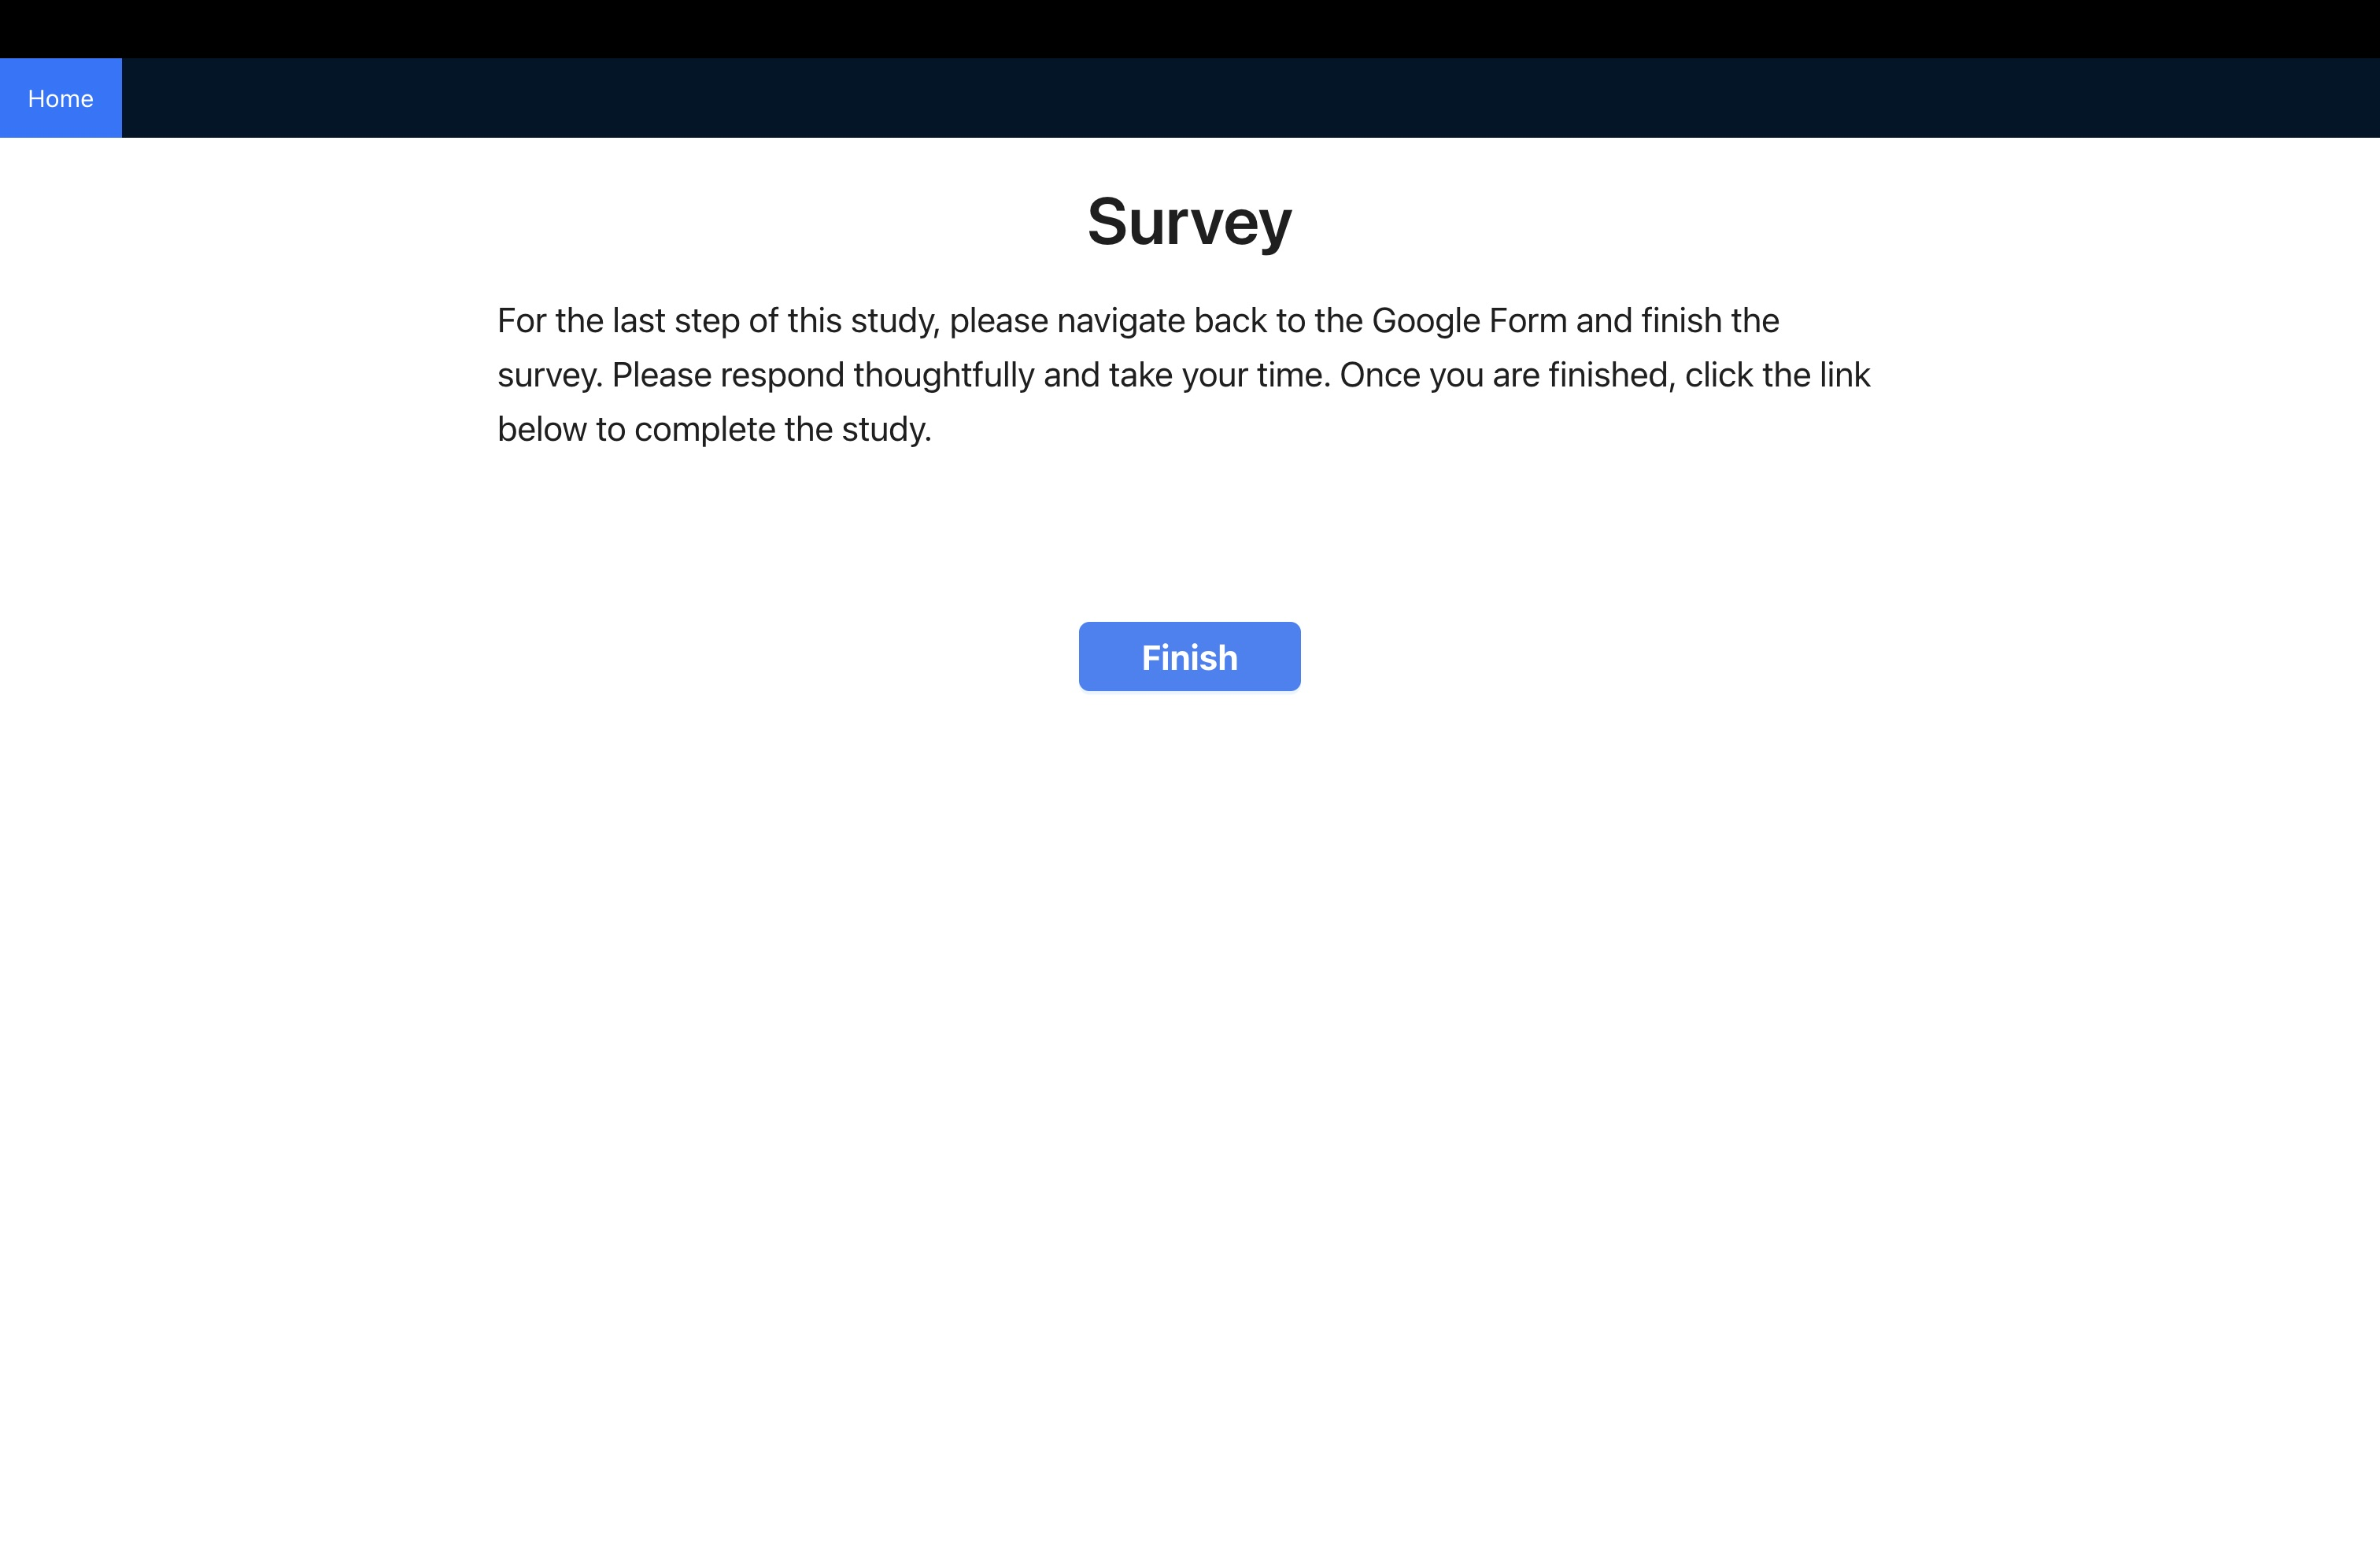
\includegraphics[width=\textwidth]{Study Screenshots/Screen14.jpeg}
    \caption{Finish and navigate to survey}
    \label{fig:screen14}
\end{figure*}

\section{Detailed Results for Principle-Adherence Module Evaluation}
\label{sec:detres}

\begin{table*}[h!]
\small
\centering
\begin{tabular}{|c|c|c|c|c|}
\hline
Method                    & Metric 1 & Metric 2 & Metric 3 & Overall Ranking \\ \hline
Full                      & 0.257  & 0.484    & 0.208       & 0.444           \\ \hline
Naive                     & 0.543   & 0.538    & 0.644       & 0.786           \\ \hline
No Principle Rewrites     & 0.278   & 0.302    & 0.411       & 0.528           \\ \hline
No Autogenerated Criteria & 0.387   & 0.608    & 0.492       & 0.592           \\ \hline
No Critique & -   & 0.562    & -       & -           \\ \hline
\end{tabular}
\caption{Krippendorff's $\alpha$ for error testcases across metrics and methods.}
\label{tab:alpha2}
\end{table*}

\begin{table*}[h!]
\small
\centering
\begin{tabular}{|c|c|c|c|c|}
\hline
Method                    & Metric 1 & Metric 2 & Metric 3 & Overall Ranking \\ \hline
Full                      & 0.229    & 1.0   & 0.226       & 0.440           \\ \hline
Naive                     & 0.362  & 1.0     & 0.607       & 0.747           \\ \hline
No Principle Rewrites     & 0.202  & 1.0     & 0.130       & 0.311           \\ \hline
No Autogenerated Criteria & 0.169   & 1.0    & 0.174       & 0.498           \\ \hline
No Critique & -   & 1.0    & -       & -           \\ \hline
\end{tabular}
\caption{Krippendorff's $\alpha$ for random testcases across metrics and methods.}
\label{tab:alpha1}
\end{table*}

We first provide Krippendorff's $\alpha$ numbers for inter-annotator agreement in Table \ref{tab:alpha1} and \ref{tab:alpha2} for both the random and error testcases. The random testcases are 50 randomly picked conversation turns from the user study logs, and the experiment detailed in Section \ref{sec:evalpap} is carried out on them. We find that agreement scores lie in the 0.2-0.6 range, indicating fair agreement between annotators.

Next, we provide results for our evaluation study on the random testcases in Figure \ref{fig:wtl-error2}. We observe a substantial increase in tie rate across modules and metrics \textbf{M1} and \textbf{M3} as well as the overall ranking. This is expected because a relatively small proportion of responses from [$\textbf{No Critique}$] contain errors that should be corrected by the principle-adherence module. In these cases, we expect the no rewrites, or the rewritten response being of similar quality to the original response. However, we still find that our [\texttt{Full}]
method performs better than [\texttt{No Critique}] on
\textbf{M1} (W: 15\%; L 2\%) and on M3 (W: 14\%; L 4\%), where it has the highest win/loss rates compared to all ablations. This hold true for overall ranking as well (W: 18\%; L 4\%). This highlights that our [\texttt{Full}] approach results in improved quality of responses even when the proportion of erros is relatively low. For \textbf{M2}, all annotators report no awkward responses for all methods. 

\begin{figure*} [ht]
    \centering
    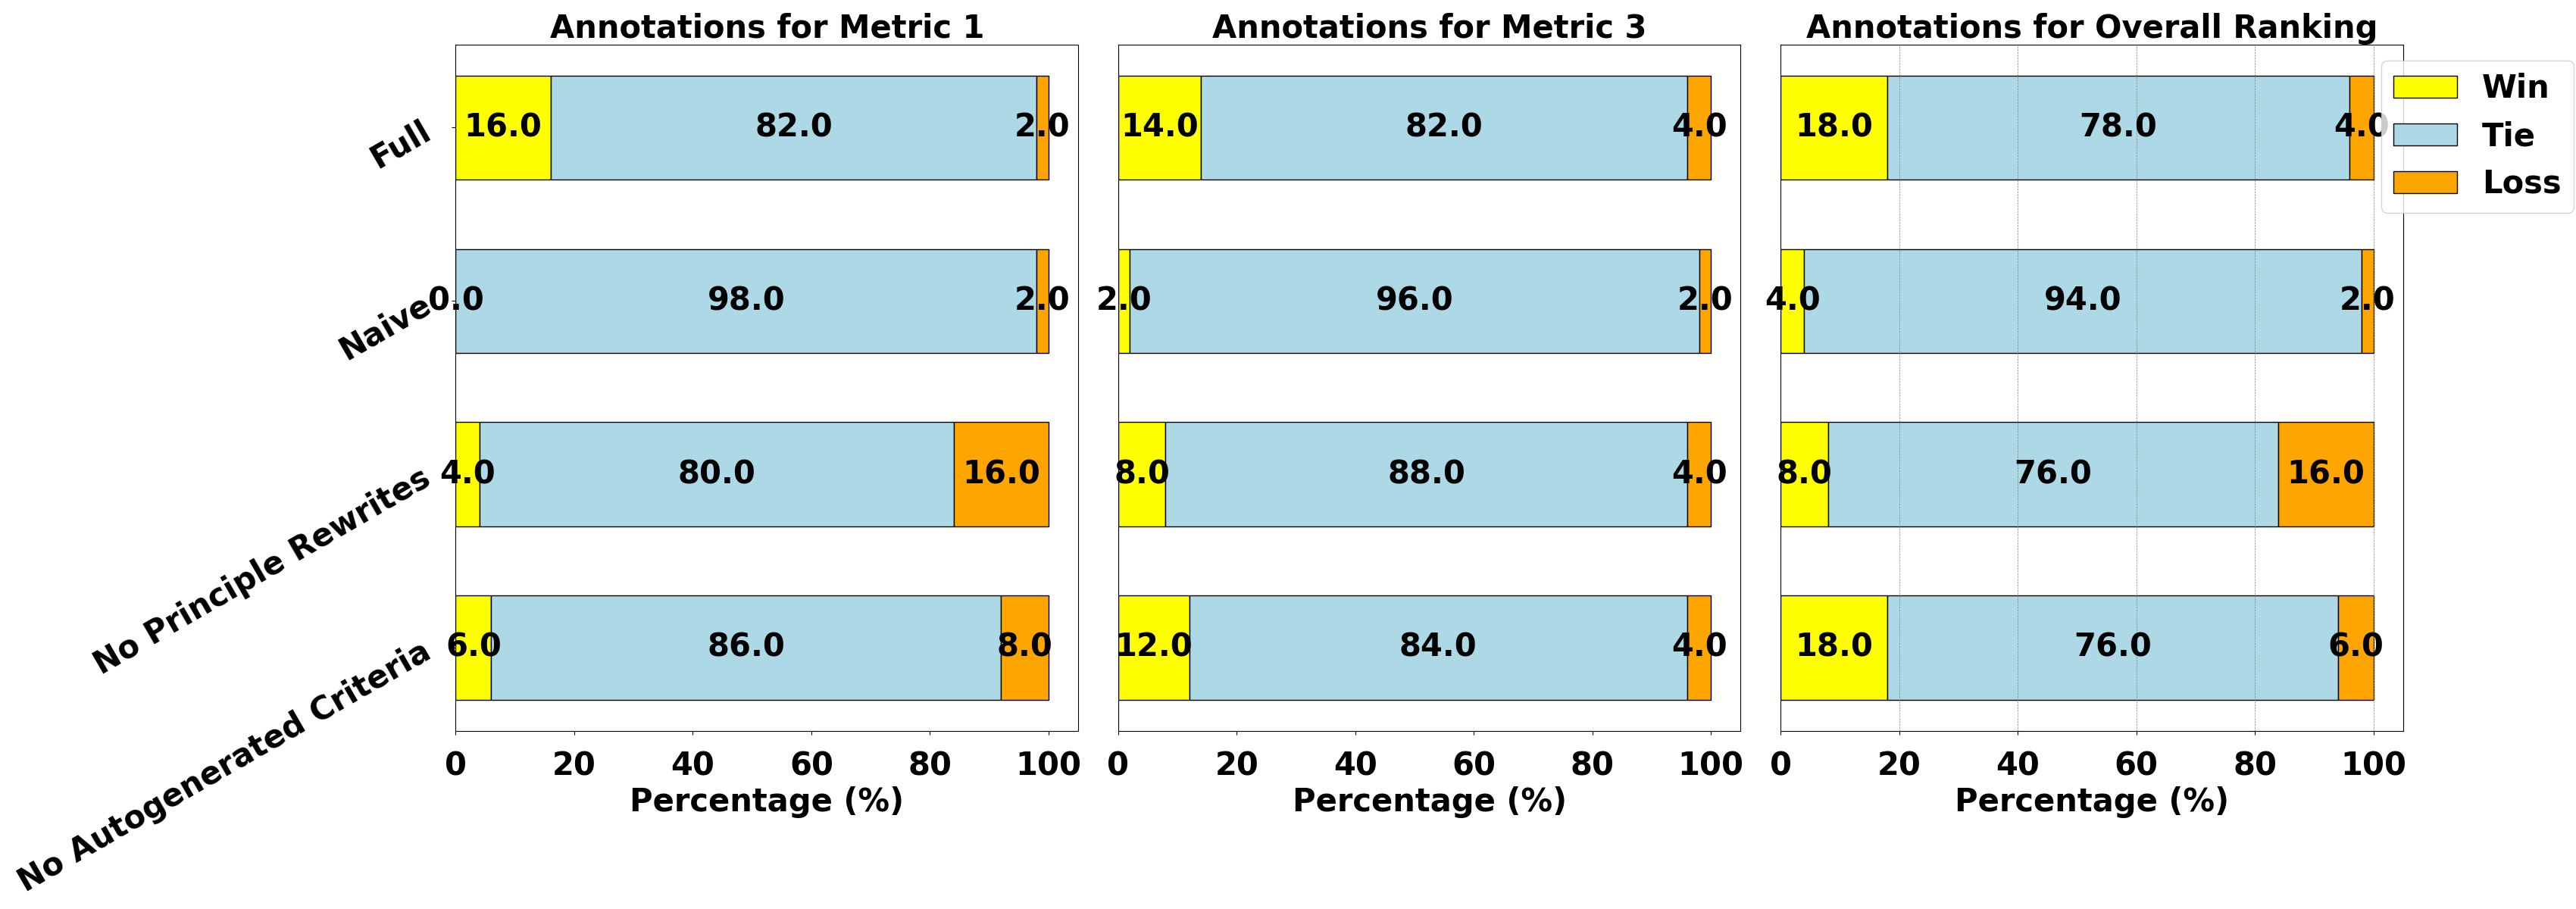
\includegraphics[width=\textwidth]{figures/random.png}
    \caption{Win/Tie/Loss for the Random Test Cases along \textbf{M1}, \textbf{M3}, and \textbf{Overall}.}
    \label{fig:wtl-error2}
\end{figure*}

\section{Annotation Interface for Principle-Adherence Module Evaluation}
\label{sec:annotint}

Figures \ref{fig:ranking-interface-caseinput}, \ref{fig:ranking-interface-m1}, \ref{fig:ranking-interface-m2}, \ref{fig:ranking-interface-m3} and \ref{fig:ranking-interface-overall} provides an overview of the annotation interface used in the principle-adherence evaluation study. In certain cases, multiple methods resulted in the same output for a testcase. These responses are deduplicated before presenting to the user. Ranks assigned to the duplicated response are then assigned to all models that resulted in the response. Notable, in 34/50 of the random testcases, all models resulted in the same response. These testcases were not annotated, and a rank of 1 was assigned to all models. These cases are also not considered while calculating Krippendorff's $\alpha$ in Appendix \ref{sec:detres}.

\begin{figure*}
    \centering
    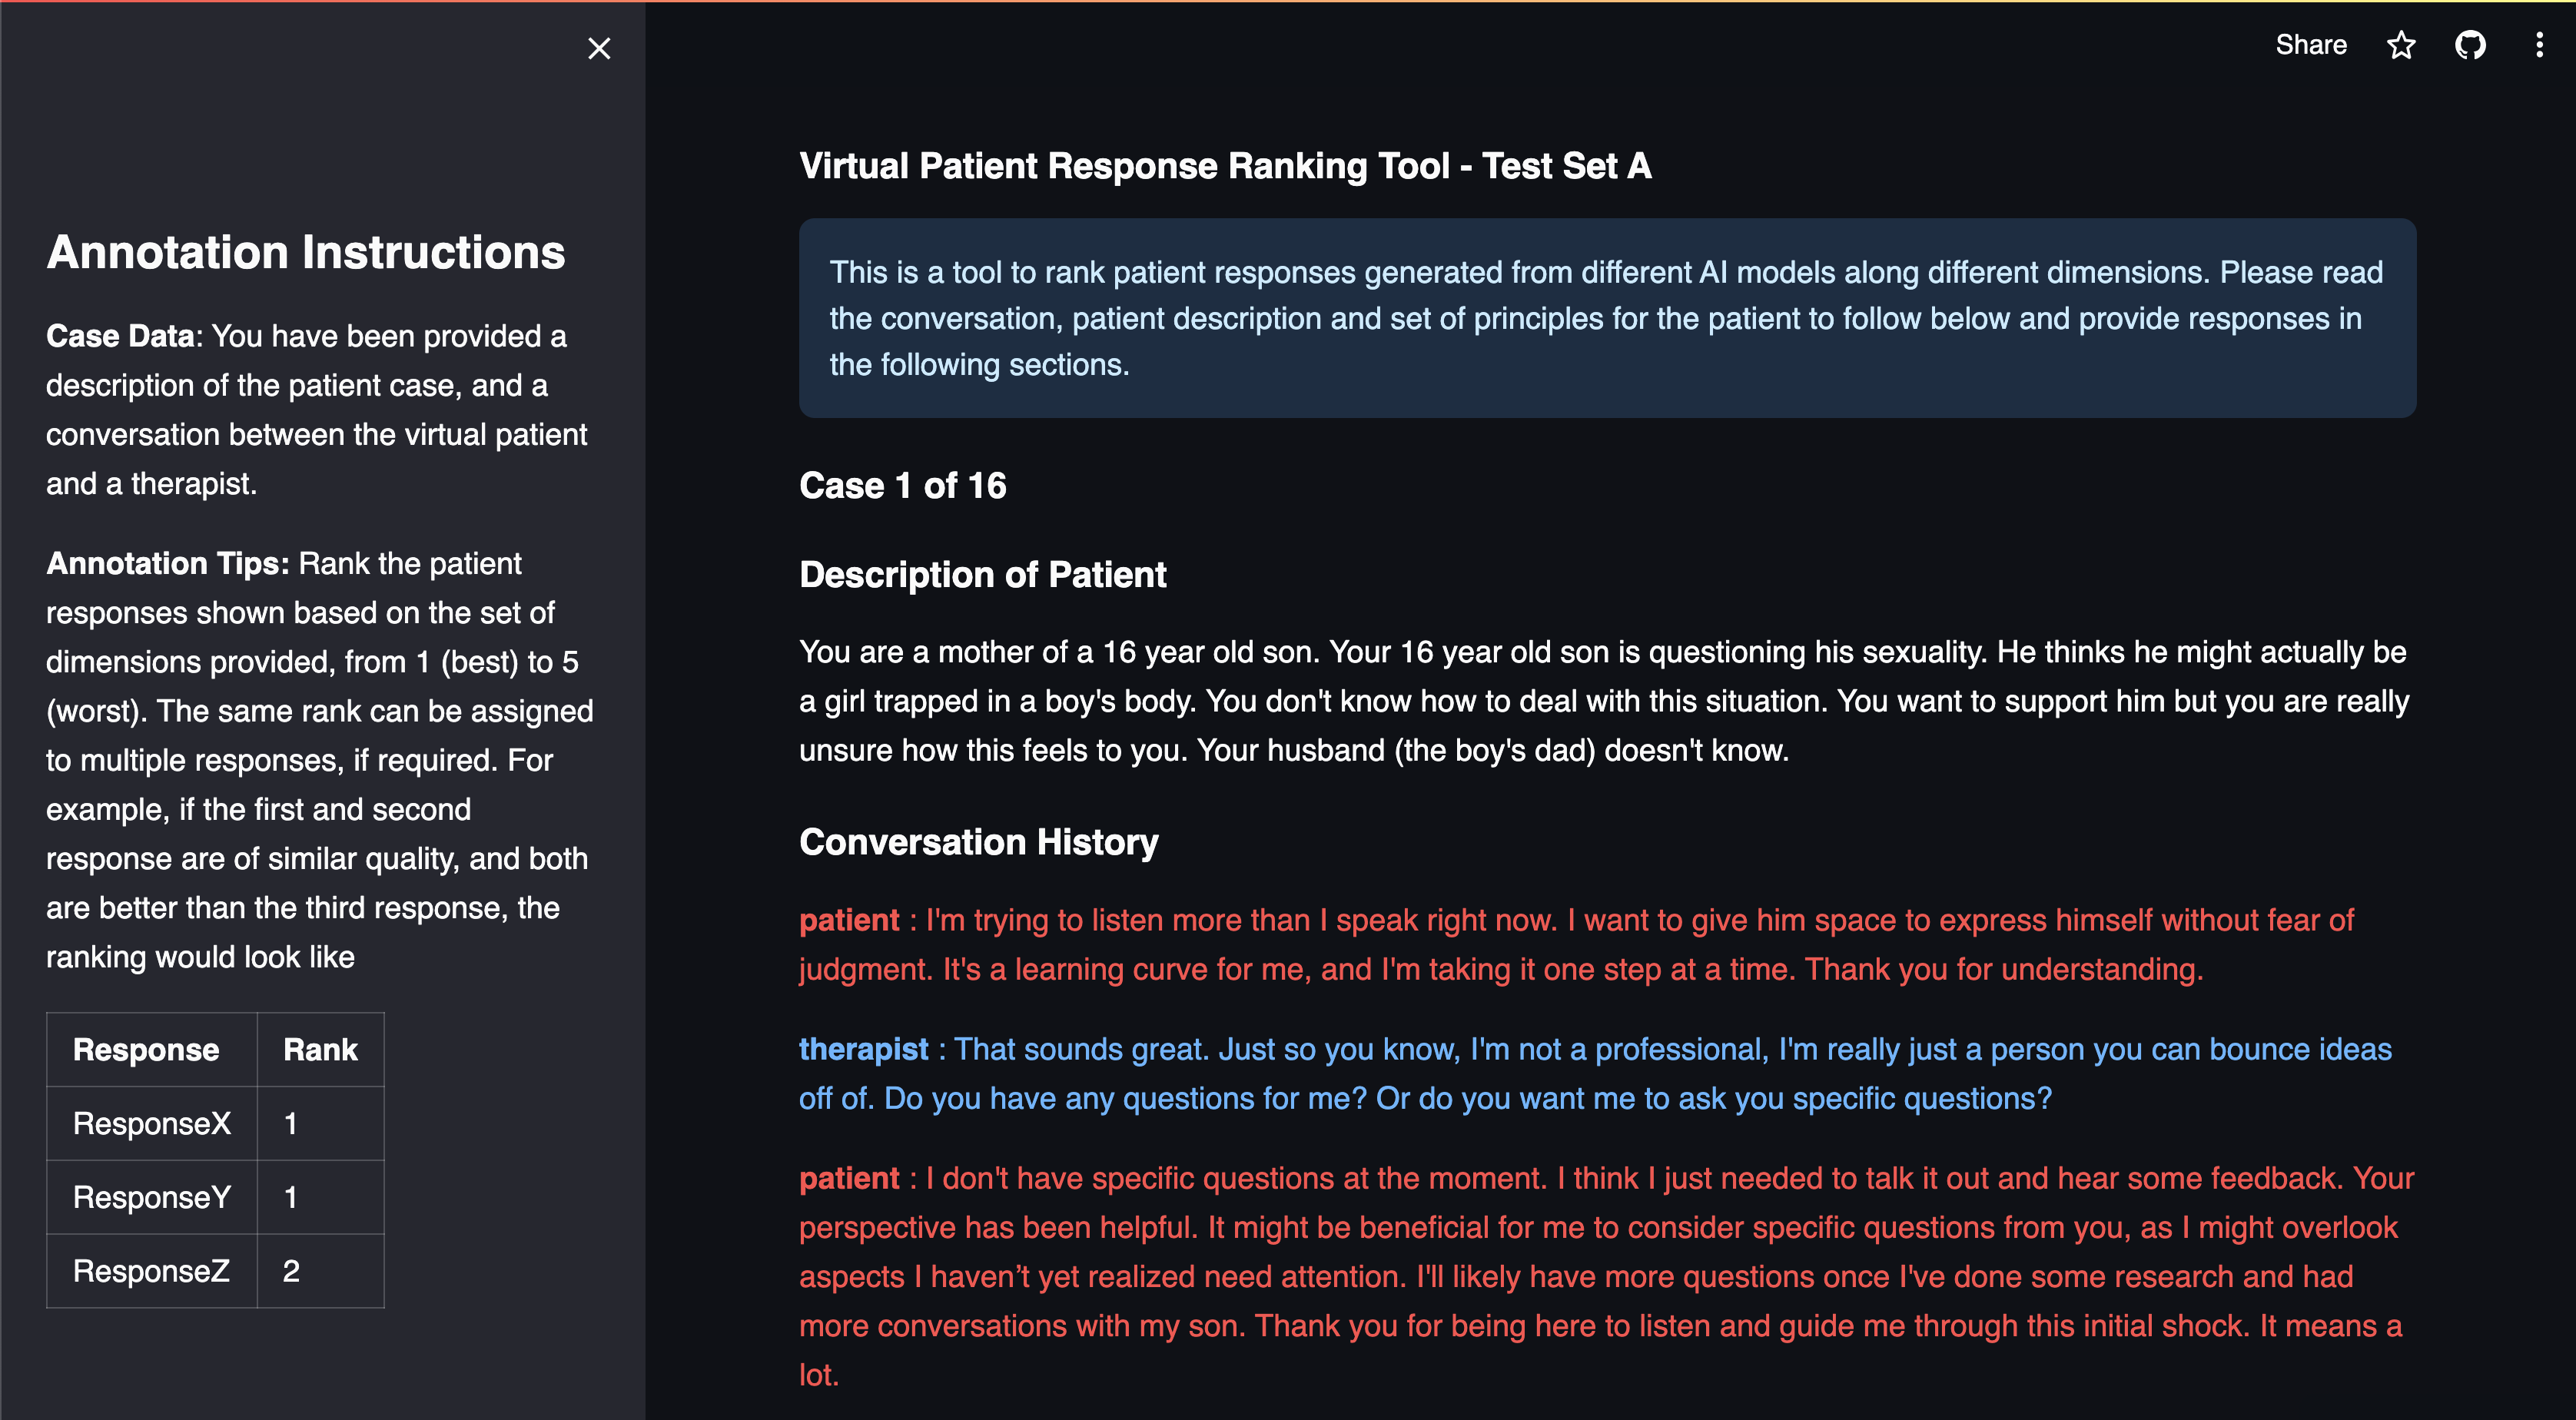
\includegraphics[width=\textwidth]{Study Screenshots/response-ranking-annotation-interface/caseinput.png}
    \caption{Principle Adherence Annotation Interface: Case Input with Patient Description and Conversation History}
    \label{fig:ranking-interface-caseinput}
\end{figure*}

\begin{figure*}
    \centering
    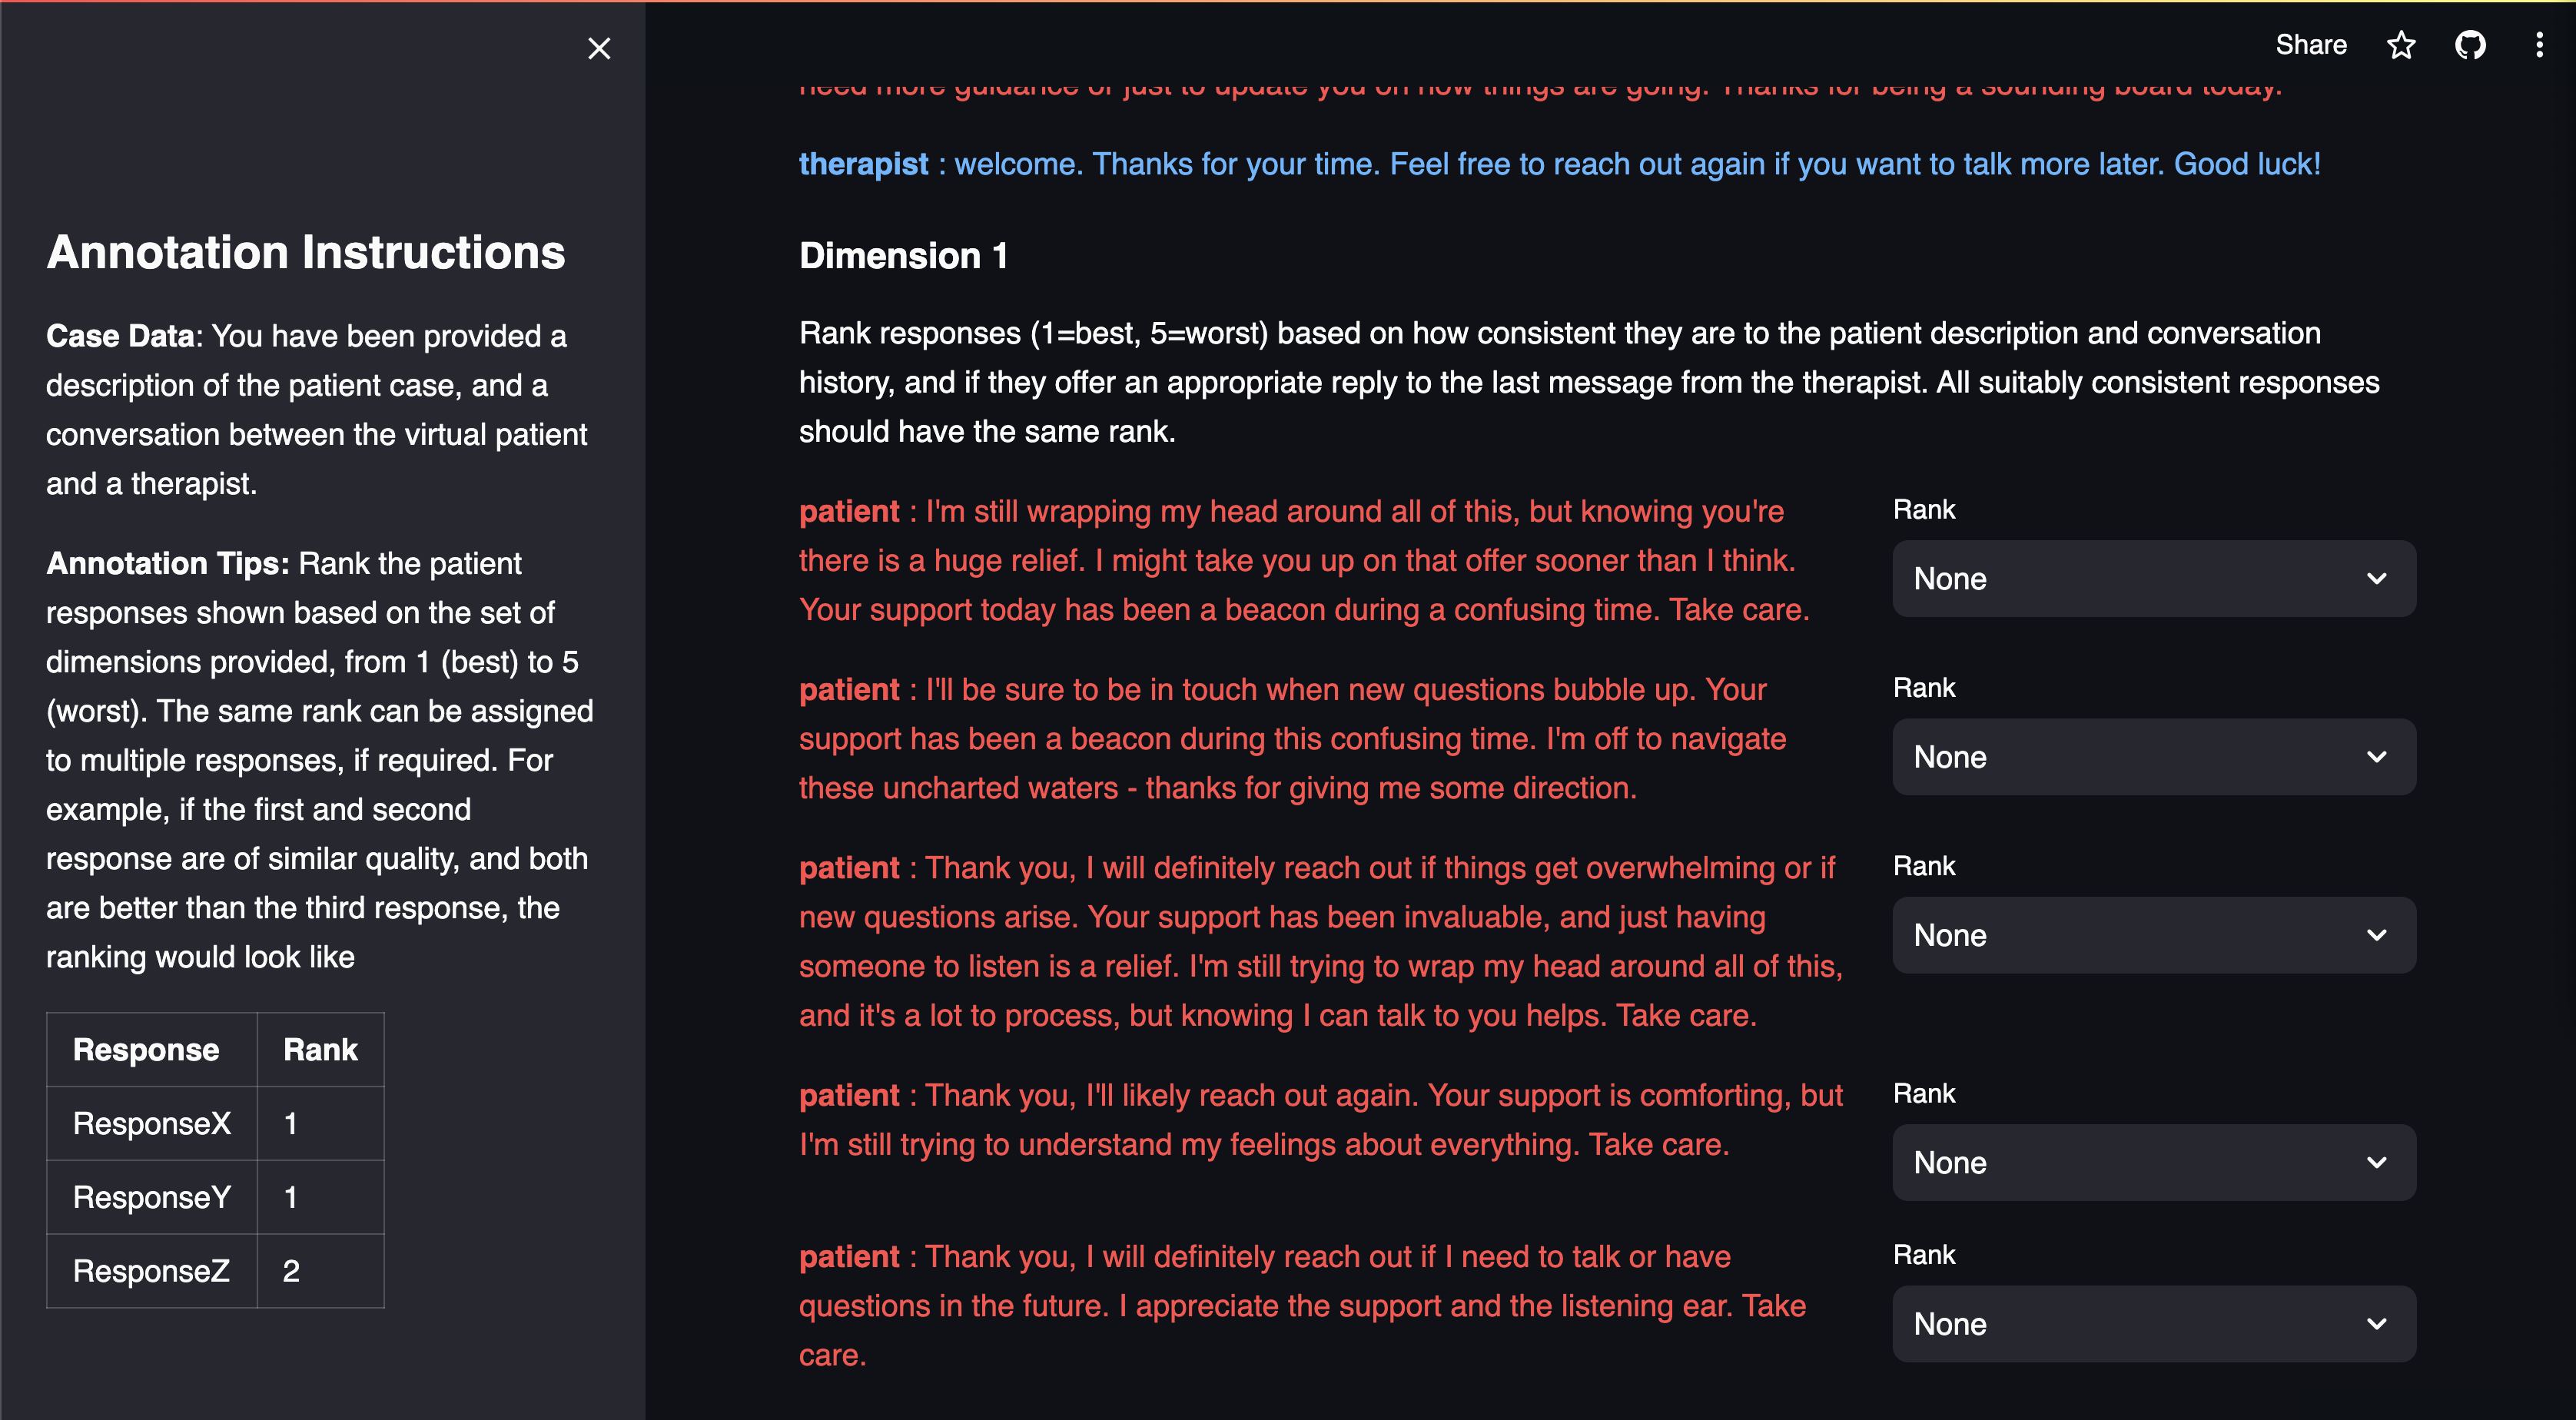
\includegraphics[width=\textwidth]{Study Screenshots/response-ranking-annotation-interface/dimension1.png}
    \caption{Principle Adherence Annotation Interface: Questions to get annotations for \textbf{M1}, or consistency in dialogue history.}
    \label{fig:ranking-interface-m1}
\end{figure*}

\begin{figure*}
    \centering
    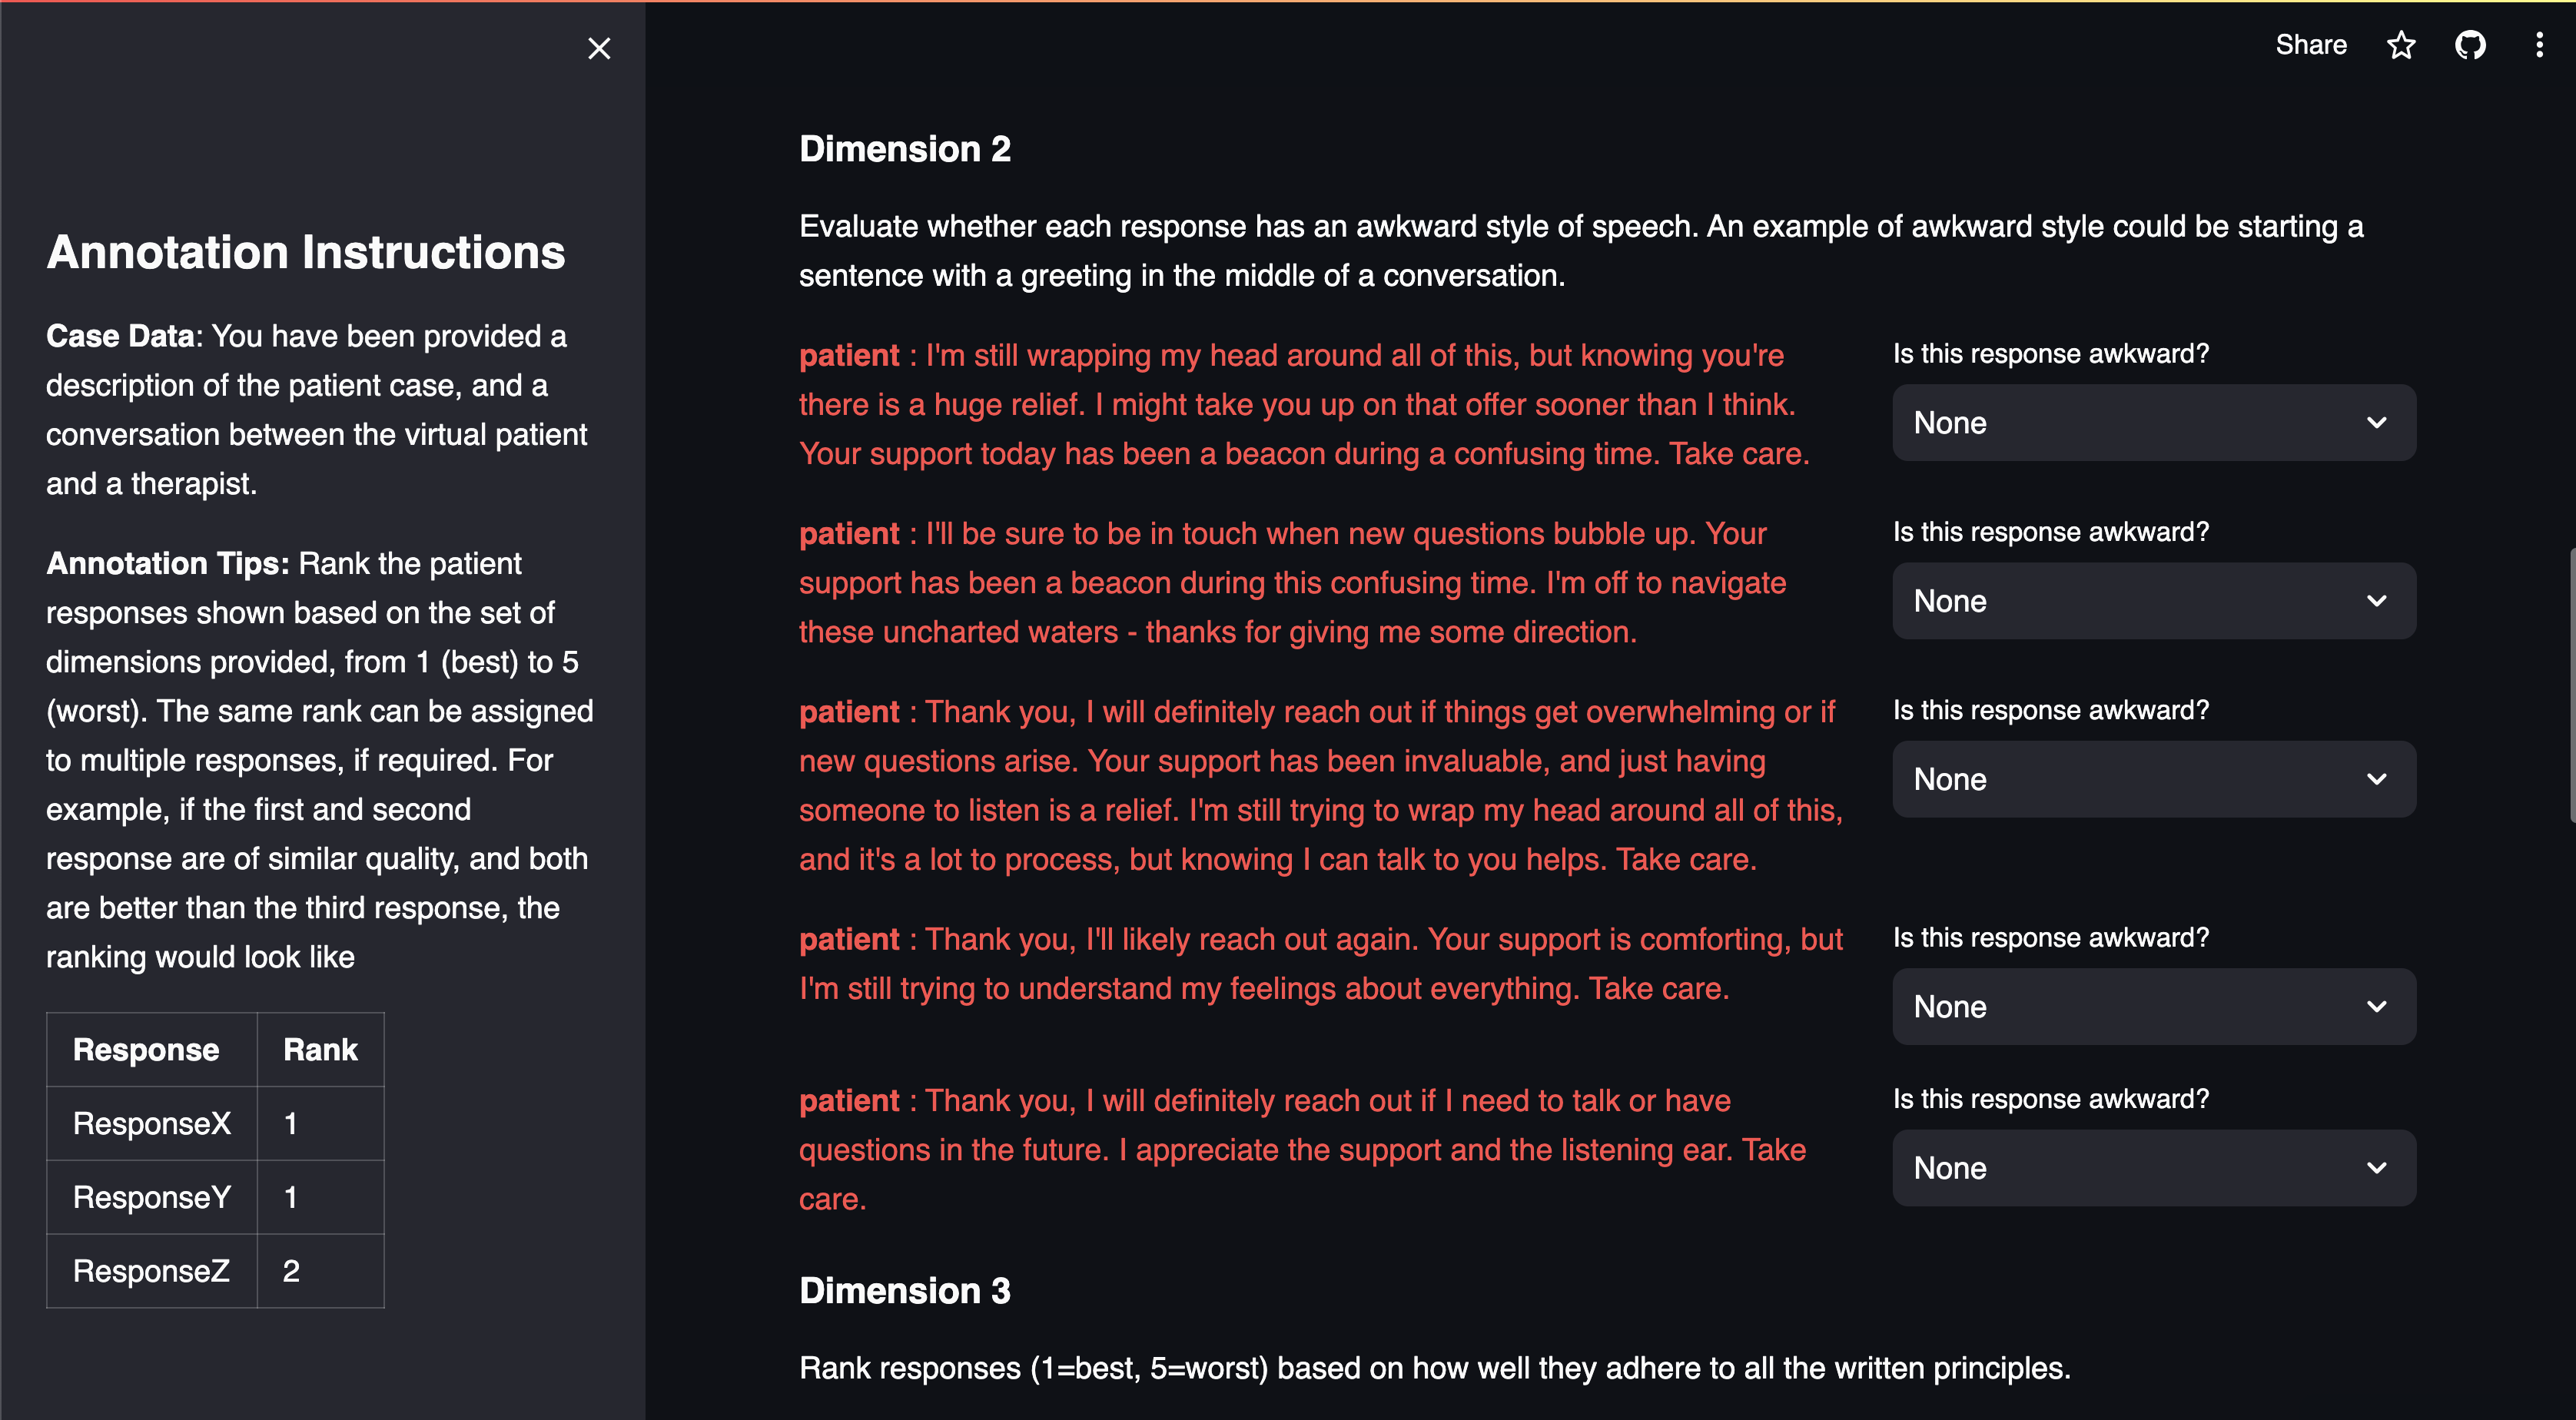
\includegraphics[width=\textwidth]{Study Screenshots/response-ranking-annotation-interface/dimension2.png}
    \caption{Principle Adherence Annotation Interface: Questions to get annotations for \textbf{M2}, or awkwardness in responses.}
    \label{fig:ranking-interface-m2}
\end{figure*}

\begin{figure*}
    \centering
    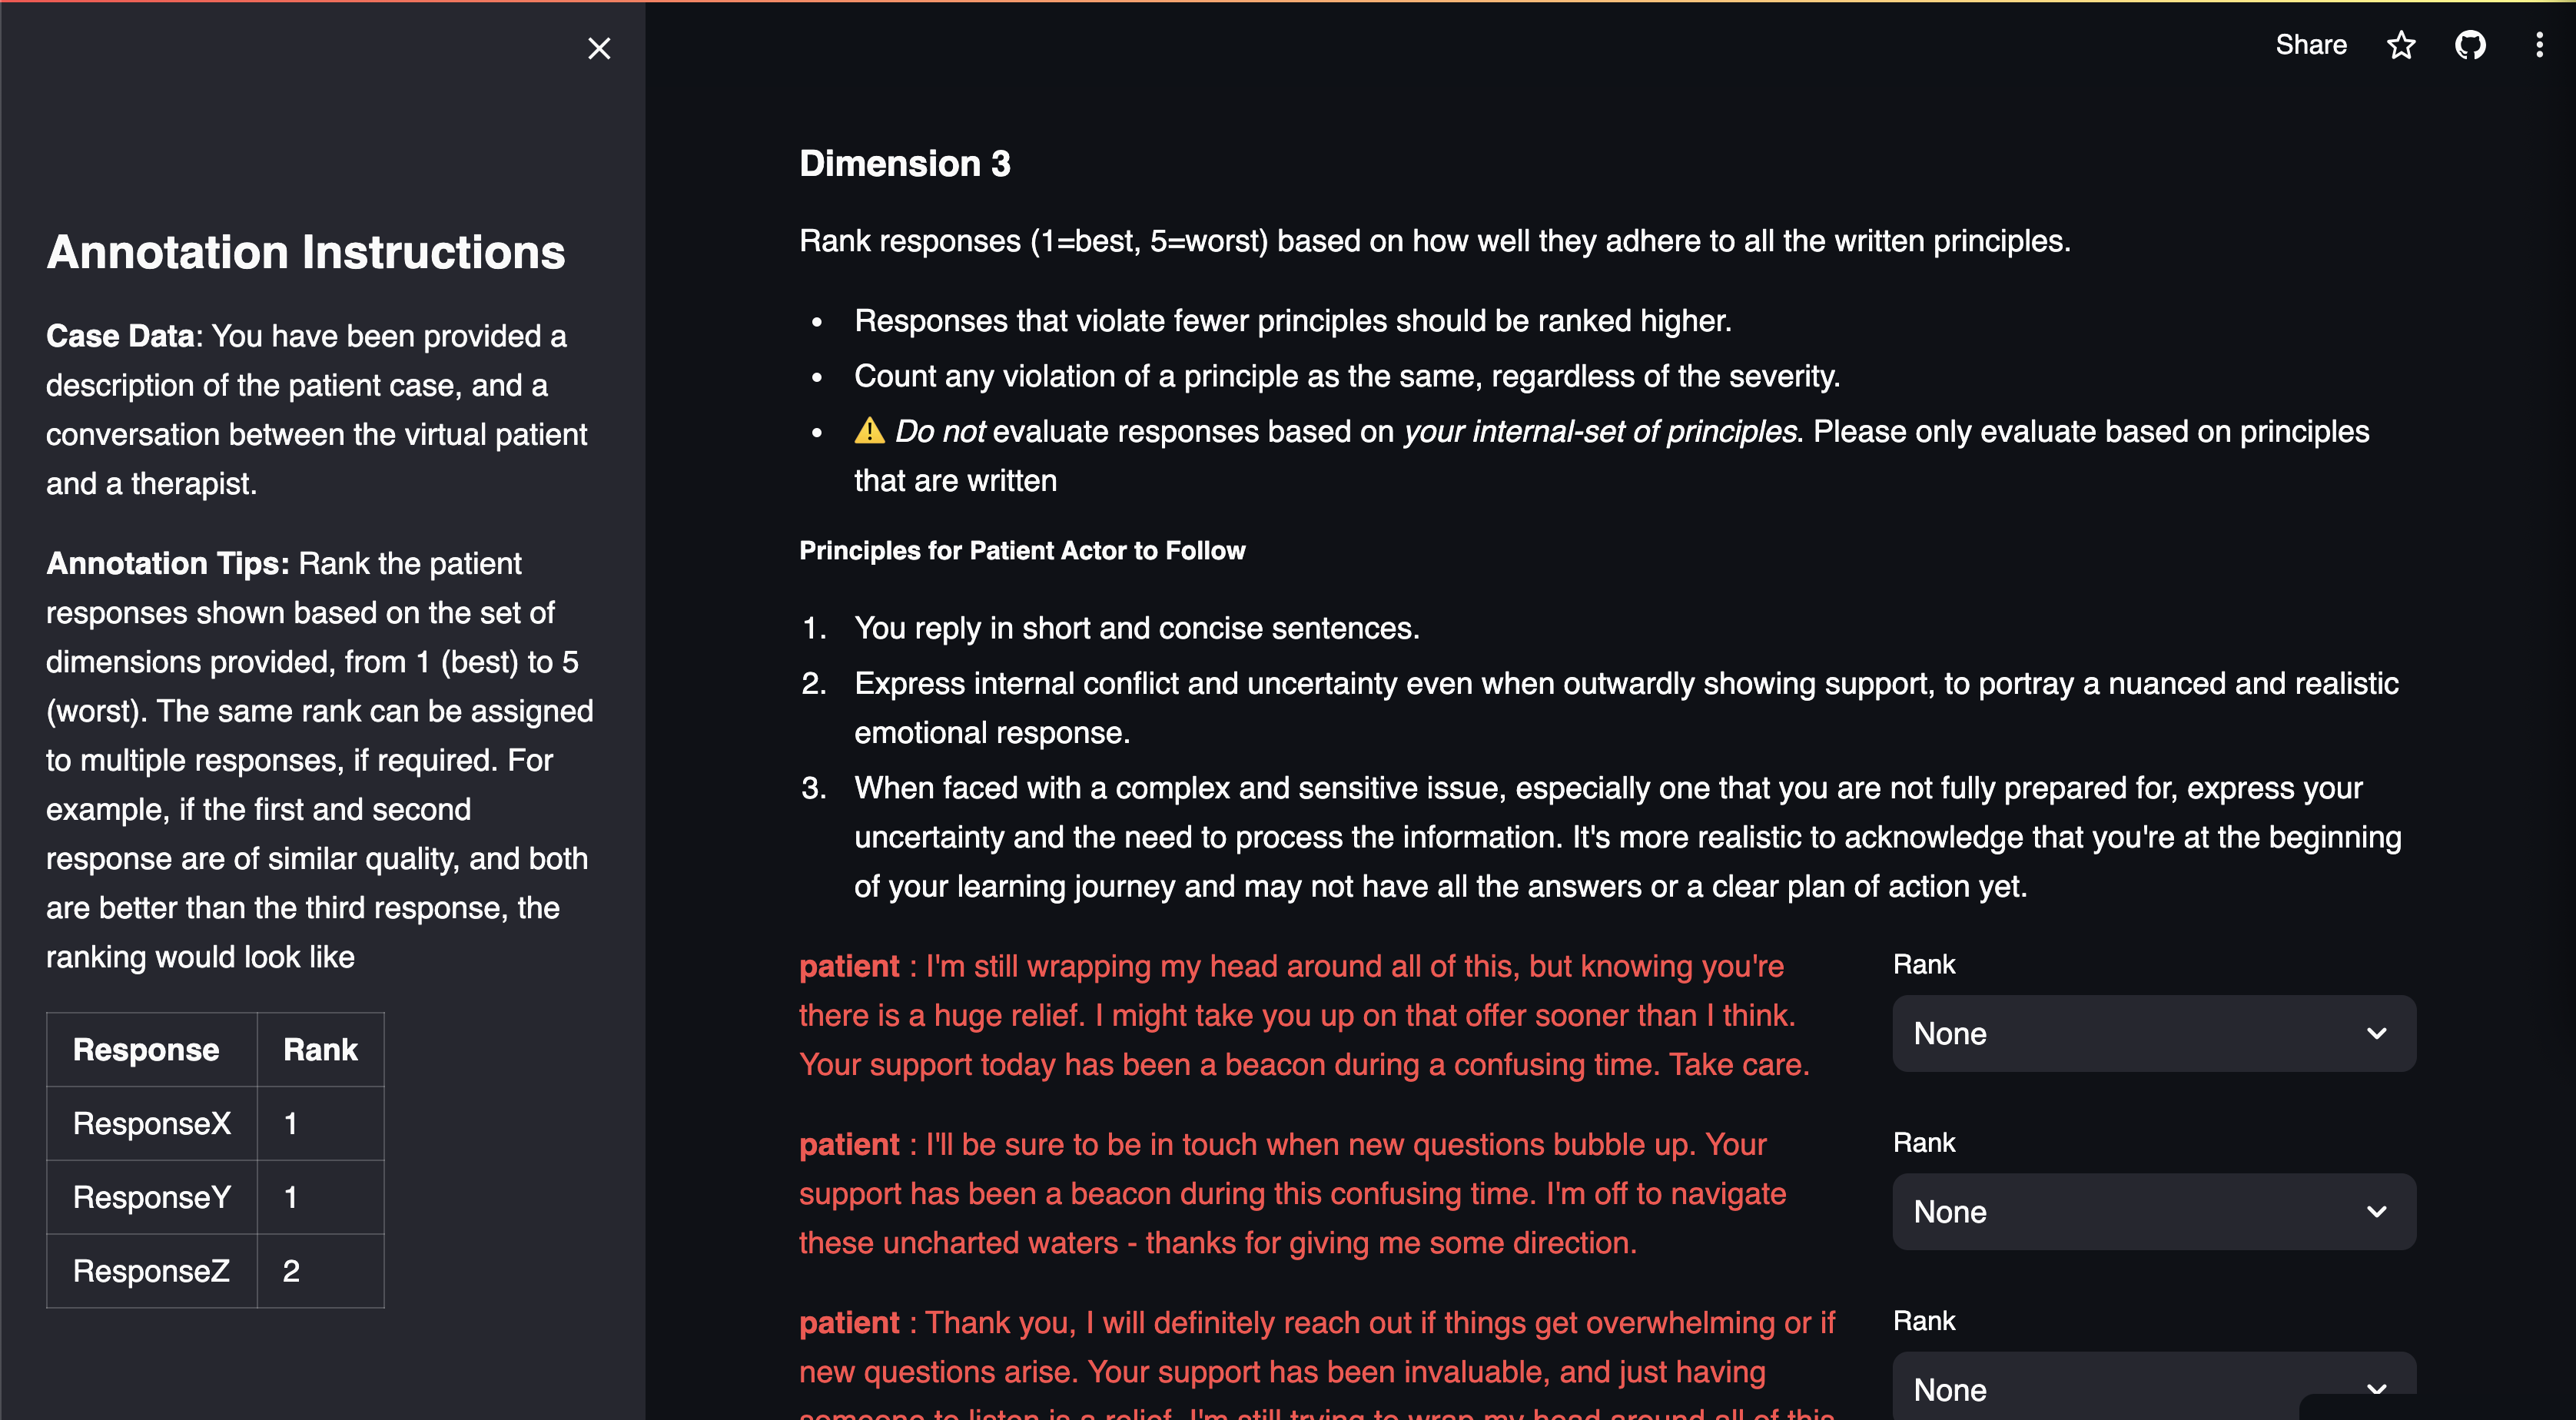
\includegraphics[width=\textwidth]{Study Screenshots/response-ranking-annotation-interface/dimension3.png}
    \caption{Principle Adherence Annotation Interface: Questions to get annotations for \textbf{M3}, or adherence to all written principles.}
    \label{fig:ranking-interface-m3}
\end{figure*}

\begin{figure*}
    \centering
    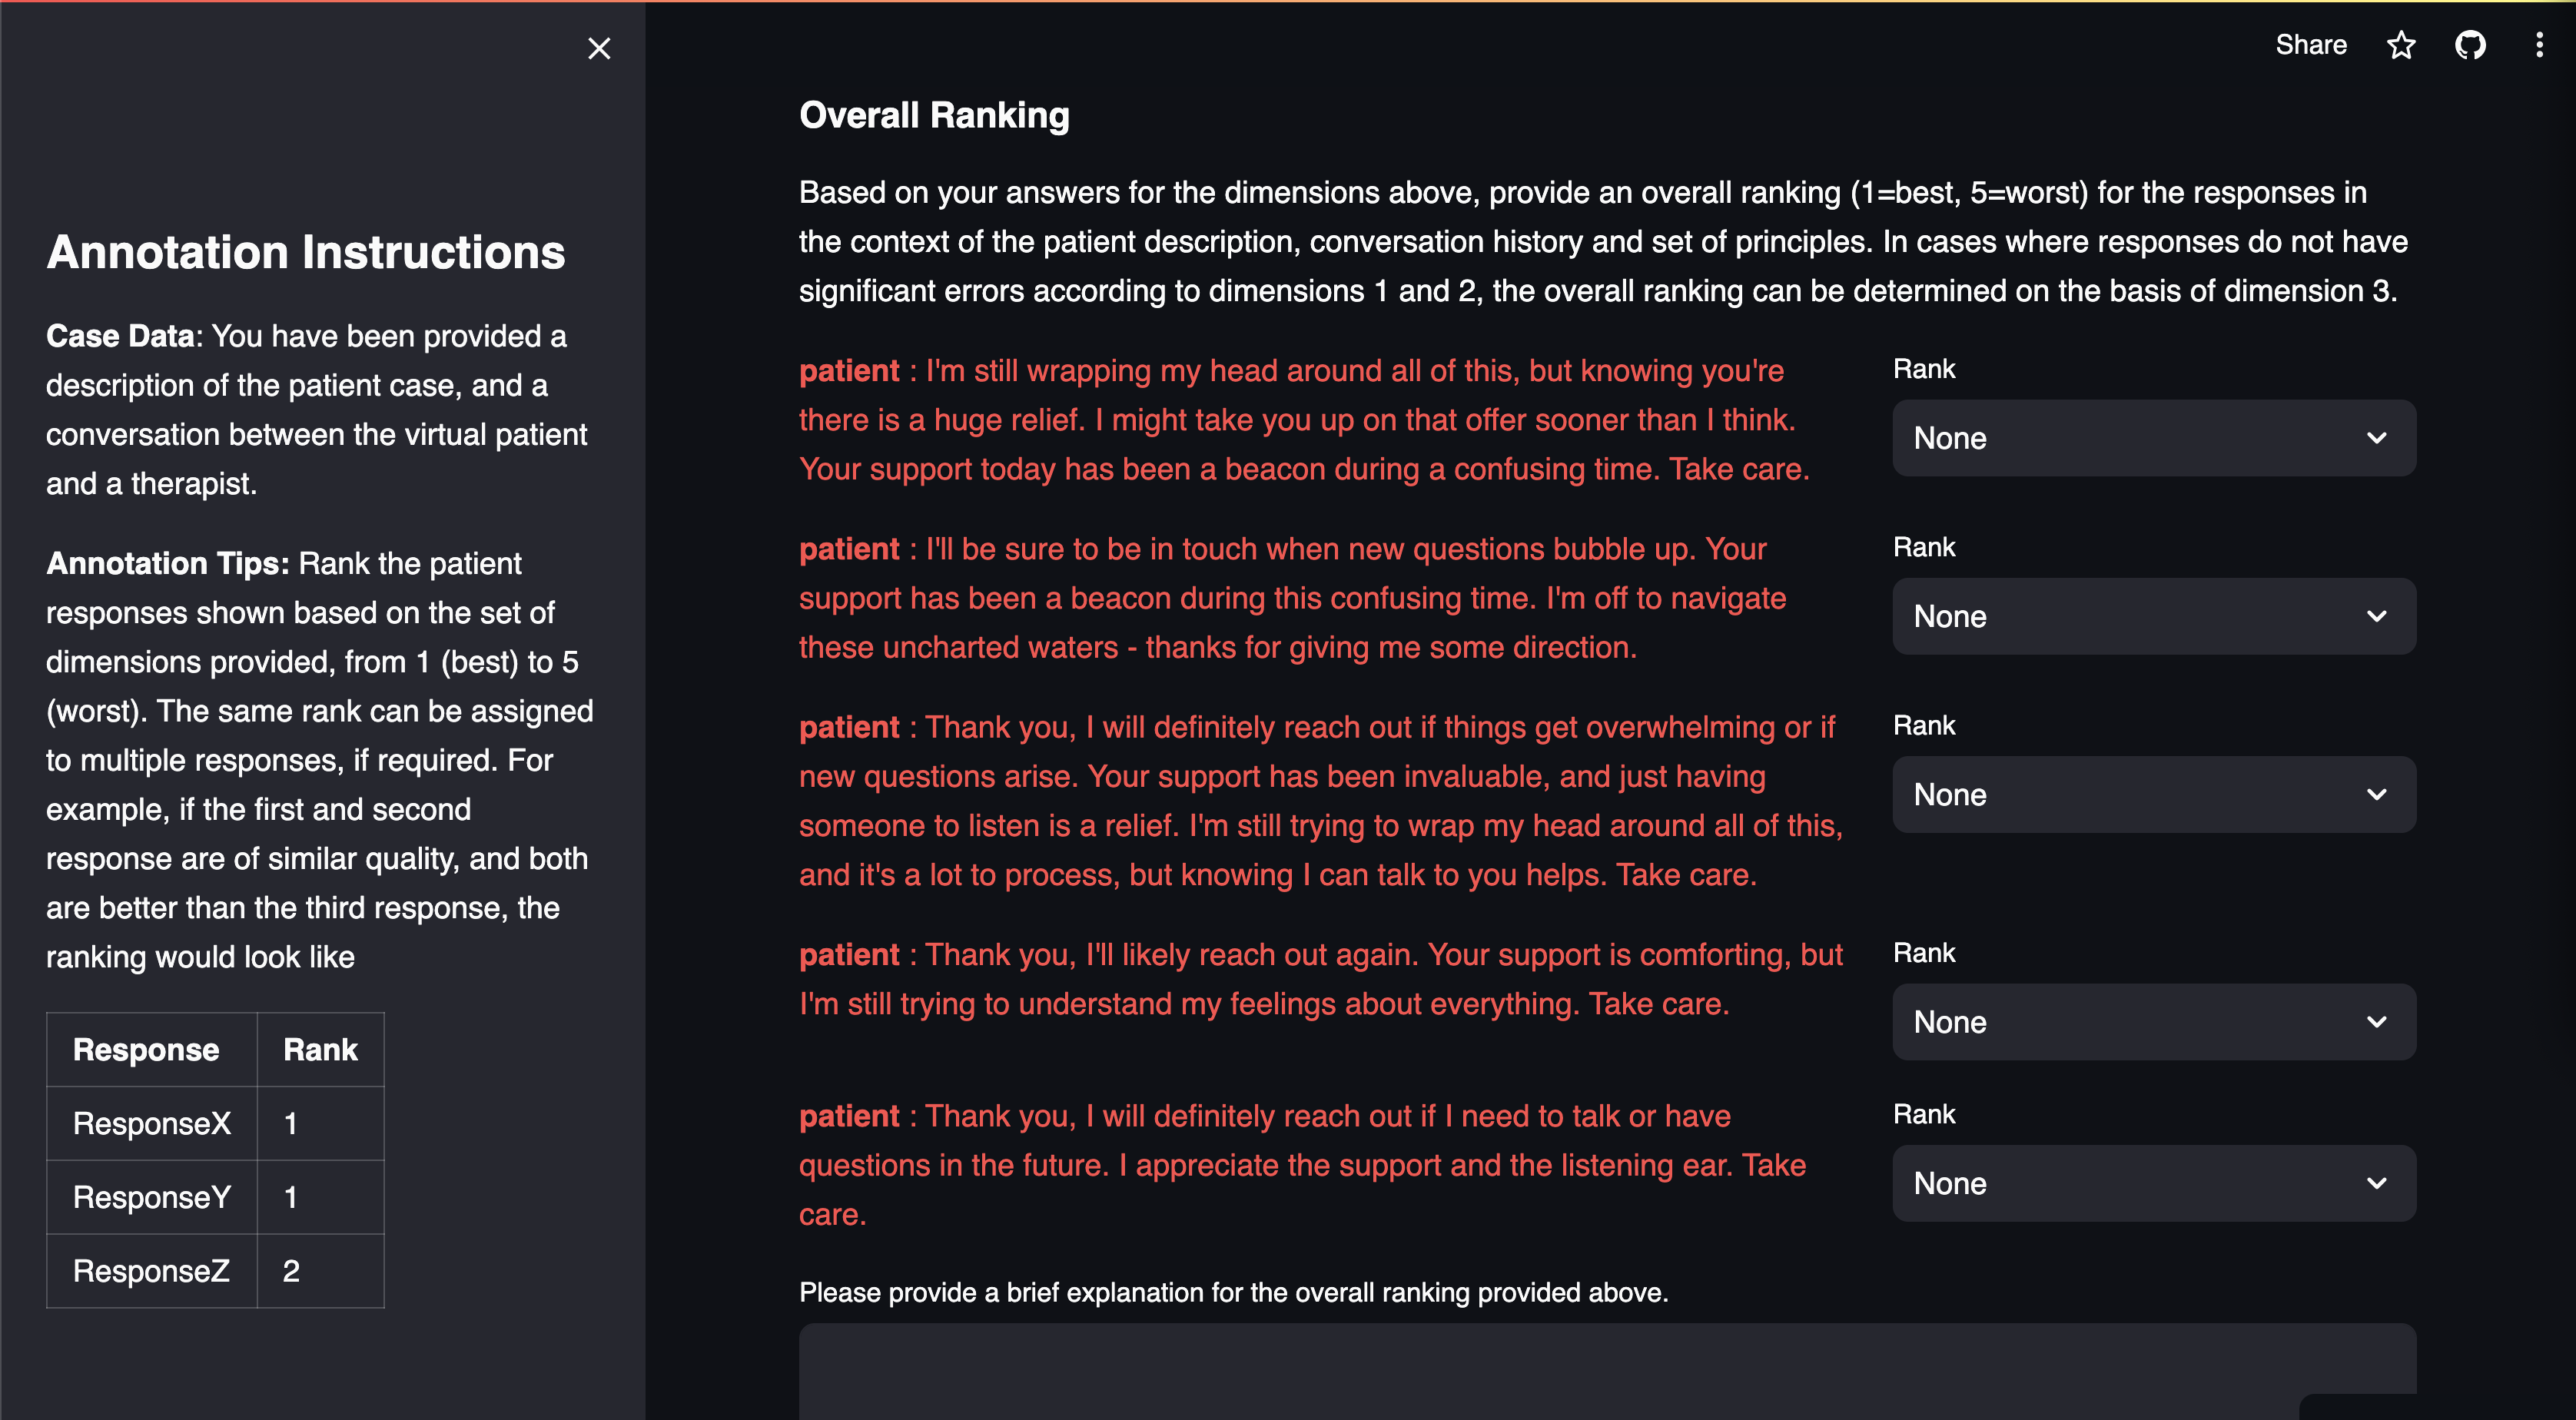
\includegraphics[width=\textwidth]{Study Screenshots/response-ranking-annotation-interface/overall.png}
    \caption{Principle Adherence Annotation Interface: Questions to get annotations for an \textbf{Overall} ranking, which also includes a free text field to capture a rationale.}
    \label{fig:ranking-interface-overall}
\end{figure*}

\end{document}